\documentclass{crescendorepchap}
%**********************************************************
%
% Bibliography support
%
%**********************************************************
%\def\@reportno{YY--NN}		% default report no.
%\def\reportno#1{\gdef\@reportno{#1}}
\RequirePackage{xspace}                 % smart spaces after macro
\usepackage[nounderscore]{syntax}
\usepackage{rotating}
\usepackage{subfigure}
\usepackage{capt-of}
\usepackage{multirow}
\usepackage{fancyhdr}
\usepackage{longtable}
\usepackage{vdmlisting}
\newcommand{\DESTECS}{\textbf{Crescendo}\xspace}

\newcommand{\bthisbibliography}[1]{\chapter*{References}%
   \begin {list} {}%
     {\settowidth {\labelwidth} {[#1]XX}%
      \setlength {\leftmargin} {\labelwidth}%
      \addtolength{\leftmargin} {\labelsep}%
      \setlength {\parsep} {1ex}%
      \setlength {\itemsep} {2ex}%
     }
  }
\newcommand{\ethisbibliography}{\end{list}}
\newcommand{\refitem}[2]
  {\bibitem[#1]{#2}}

\newcommand{\back}{$\setminus$}
\newcommand{\RuleTarget}[1]{\hypertarget{rule:#1}{}}
\newcommand{\Ruledef}[2]
{
  \RuleTarget{#1}\Rule{#1}{#2}%
  }
\newcommand{\Ruleref}[1]{
  \hyperlink{rule:#1}{#1}}
\newcommand{\Lit}[1]{`{\tt #1}\Quote}
\newcommand{\Rule}[2]{
  \begin{quote}\begin{tabbing}
    #1\index{#1}\ \ \= = \ \ \= #2  ; %    Adds production rule to index

  \end{tabbing}\end{quote}
  }
%%%%%%%%%%%%%%%%%%%%%%%%%%%%%%%%%%%%%%%%%%%%%%%%%%%%%%%%%%%%%
%%% Model transformation rule box
%%%%%%%%%%%%%%%%%%%%%%%%%%%%%%%%%%%%%%%%%%%%%%%%%%%%%%%%%%%%%
\newcounter{formationRule}
\setcounter{formationRule}{0}
\newenvironment{formationRule}
%{\refstepcounter{formationRule}\vspace{10pt}\par\noindent
%Exercise \theformationRule
%\begin{itshape}\par\noindent\vspace{10pt}}%
%{\end{itshape}\vspace{10pt}\par}
{%
\refstepcounter{formationRule}
%increment
%\addtocounter{transformationRuleCounter}{1}%
%\ctf{}%
%\labelformat{formationRule}{\value{formationRule}}
\begin{center}%
\begin{tabular}{ | p{10cm} |}\hline%
\textbf{Transformation Rule \theformationRule}

}
{
\\
    \hline
    \end{tabular}
\end{center}

}
\newcommand{\kw}[1]{{\textbf\ttfamily #1}}
\newcommand{\SeqPt}[1]{\{\ #1\ \}}
\newcommand{\lfeed}{\\ \> \>}
\newcommand{\dsepl}{\ $|$\ }
\newcommand{\dsep}{\\ \> $|$ \>}
\newcommand{\Lop}[1]{`{\sf #1}\Quote}
\newcommand{\blankline}{\vspace{\baselineskip}}
\newcommand{\Brack}[1]{(\ #1\ )}
\newcommand{\nmk}{\footnotemark}
\newcommand{\ntext}[1]{\footnotetext{{\bf Note: } #1}}
\newlength{\kwlen}
\newcommand{\Keyw}[1]{\settowidth{\kwlen}{\tt #1}\makebox[\kwlen][l]{\sf
    #1}}
\newcommand{\keyw}[1]{{\sf #1}}
\newcommand{\vdmkeyw}[1]{{\bf\ttfamily #1}}

\newcommand{\id}[1]{{\tt #1}}
\newcommand{\metaiv}[1]{\begin{alltt}\input{#1}\end{alltt}}

\newcommand{\OptPt}[1]{[\ #1\ ]}
\newcommand{\MAP}[2]{\kw{map }#1\kw{ to }#2}
\newcommand{\INMAP}[2]{\kw{inmap }#1\kw{ to }#2}
\newcommand{\SEQ}[1]{\kw{seq of }#1}
\newcommand{\NSEQ}[1]{\kw{seq1 of }#1}
\newcommand{\SET}[1]{\kw{set of }#1}
\newcommand{\PROD}[2]{#1 * #2}
\newcommand{\TO}[2]{$#1 \To #2$}
\newcommand{\FUN}[2]{#1 \To #2}
\newcommand{\PUBLIC}{\ifthenelse{\boolean{VDMpp}}{public\mbox{}}{\mbox{}}}
\newcommand{\PRIVATE}{\ifthenelse{\boolean{VDMpp}}{private}{\mbox{}}}
\newcommand{\PROTECTED}{\ifthenelse{\boolean{VDMpp}}{protected}{\mbox{}}}

\pagestyle{fancy}
\fancyhead{}
\fancyhead[LO]{\leftmark}
\fancyhead[RE]{Crescendo Examples Compendium}
\fancyhead[RO,LE]{\resizebox{0.05\textwidth}{!}{
\includegraphics{crescendo_logo_512}}}
\fancyfoot[C]{\thepage}

\usepackage{makeidx}

\usepackage{graphicx, color}

% definition of VDM++, JavaCC, JJTree, JTB, ANTLR and SableCC for listings
\newcommand{\NL}{\mbox{}\\ \vspace*{-5mm}}
\usepackage{listings}
\usepackage{listingsDCL}
\newcommand{\url}[1]{\texttt{#1}}
%\usepackage{vdmsl-2e}
\usepackage{hyperref}

\usepackage{times}
\usepackage{color}

%\include{ifad}
%\include{graphics}
\usepackage{cite}
\usepackage{alltt}
%\usepackage{fancyhdr}
\renewcommand{\topfraction}{0.9}
\renewcommand{\textfraction}{0.05}
\renewcommand{\floatpagefraction}{0.9}
\makeindex

%\input{include/settings}

% Defining deadline command
\newcommand{\deadline}[3]{
\fbox{Responsability: #1} \\
\fbox{Full Draft: #2} \\
\fbox{Final Version: #3}
}

\begin{document}
\title{Crescendo Examples Compendium}
\author{Claire Ingram, Ken Pierce, Carl Gamble, \\[5mm]
Sune Wolff, Martin Peter
Christensen and Peter Gorm Larsen\\
Aarhus University, Department of Engineering\\
Finlandsgade 22, DK-8200 Aarhus N, Denmark
}

\date{January 2014}

\reportno{TR-002}

\maketitle
%\makerro

\frontmatter

\textbf{Document history}

\begin{tabular}{|l|l|l|l|}\hline
Month   & Year & Version & Version of Crescendo.exe \\ \hline
December& 2012 & 1       & 1.1.8 (then called DESTECS)  \\ \hline
January& 2014 & 2       & 2.0.0 \\ \hline
\end{tabular}
%\maketitle

\cleardoublepage

%\input{Abstract}

\cleardoublepage

% The front matter starts here

%\include{Summary}

%\include{Preface}

% In a two-sided printing style, it makes the next page a right-hand
% (odd-numbered) page, producing a blank page if necessary.
%\cleardoublepage

% Add the table of contents pages (TOC)
\tableofcontents


% The report body, i.e. the main matter, starts here
\mainmatter
\chapter{Introduction}\label{cha:intro}
This deliverable provides an overview of different public example
co-models that stakeholders who are interested in experimenting with
the \DESTECS technology can use as a starting point\footnote{The corresponding
sources of all the examples can be found
at~\url{http://www.destecs.org/downloads.html}}.

This deliverable is structured in different chapters, each of which
provides a brief (2 to 3 pages) introduction to one example model.
Depending upon your own background and your interest in exploring the
DESTECS technology and the particular features that interest you, you
may wish to start with a different chapter than that presented first. The
different chapters and the examples they present illustrate different
aspects as explained here:

\begin{itemize}
\item Chapter~\ref{chap:controllerPattern} illustrates the
  \emph{Simple Controller}.  This example may be of particular
  interest to those with a background in CT modelling who want to see
  how to convert an existing CT model to a DESTECS co-model.
\item Chapters \ref{chap:watertankperiodic} and
  \ref{chap:watertankeventdriven} present two different models of a
  water tank which maintains a given water level.  Chapter
  \ref{chap:watertankperiodic} describes a model which in which the
  controller periodically polls the sensor for the current state,
  whilst Chapter \ref{chap:watertankeventdriven} describes a similar
  model that employs an event-driven solution to the same problem.
\item Chapter~\ref{chap:pidPinch} presents a small example with a pair
  of rollers used inside a printer (called ``pinches''). This example
  is of particular relevance for those who are interested in different
  types of faults and alternative fault tolerance techniques.
\item Chapter~\ref{chap:fuelSystem} presents a fuel system for an
  aircraft. This example has been used in other formalisms as well and
  different faulty scenarios are also considered.
%\item Chapter~\ref{chap:pacemaker} describes a pacemaker device, that
% monitors a human heart and intervenes to regulate the heart rate if
% it detects irregularities in the heart's natural beat.  The
%  pacemaker models the behaviour of a healthy heart, and also several
 % different irregularities.
\item Chapter \ref{chap:morsecodereader} describes a decoder which can
  translate messages presented in Morse code (as ``dots'' and
  ``dashes'' on a strip of tape) into Latin characters.  This example
  demonstrates the use of shared design parameters to test model
  performance in different environmental conditions (such as varying
  levels of background noise).
\item Chapter~\ref{chap:lineFollowingRobot} illustrates a
  line-following robot. This example demonstrates how the DESTECS
  technology can support design space exploration using an Automated
  Co-model Analysis (ACA). Here it is used to analyse alternative
  placements of different light sensors.
\item Chapter \ref{chap:summerschoolmodels} expands on Chapter
  \ref{chap:lineFollowingRobot}.  It presents five further co-models
  of a line-following robot, each developed independently by attendees
  at the 2012 DESTECS summer school.  Each co-model exhibits different
  design choices and optimisations for solving the same problems and
  so these models are interesting to study side-by-side for those
  interested in exploration of the design space.
\item Chapters \ref{chap:chesswaysimple}, \ref{chap:chesswaysl} and
  \ref{chap:chesswaydestecs} present progressively more complex models
  of a self-balancing scooter, called a Chessway.  Chapter
  \ref{chap:chesswaysimple} describes a very simple model that
  includes basic functionality only.  Chapter
  \ref{chap:chesswaydestecs} describes a more complex model of the
  same scooter.  The latter includes some components linked over a
  wireless connection, and so it also demonstrates some fault tolerant
  techniques.  The plant model for this particular model is larger
  than many other examples.  Chapter \ref{chap:chesswaysl} presents an
  intermediate model which bridges the gap between the simple model
  and the more complex one. It includes a DE model only, which has
  been developed in order to answer some key design questions
  necessary before the model in Chapter \ref{chap:chesswaydestecs} can
  be built.
\end{itemize}

In order to guide you as to which models to consider inspecting we
have created a table illustrating the different characteristics of the
various co-models available (see Table~\ref{tab:characteristics});
characteristics which might be of interest include scripted scenarios,
fault tolerance, Automated Co-model Analysis (ACA), 2D/3D animation,
and patterns which have been implemented in each model.  For more on
patterns, see DESTECS deliverable D2.3~\cite{DESTECSD23}.  Some models here have been implemented entirely as a DE model (e.g., entirely in VDM, with no 20-sim component), or entirely as a CT model (e.g., entirely in 20-sim, with no VDM component).  We indicate whether this applies in Table \ref{tab:characteristics}, with \emph{CT alone enabled} or \emph{DE alone enabled}.

\begin{table}[!h]
\begin{centering}
\begin{tabular}{|l|c|c|c|c|c|c|c|c|c|}\hline
Co-model(s)
&\begin{sideways}Event triggered\end{sideways}
&\begin{sideways}CT alone enabled\end{sideways}
&\begin{sideways}DE alone enabled\end{sideways}
&\begin{sideways}Scenarios included\end{sideways}
&\begin{sideways}CT faults included\end{sideways}
&\begin{sideways}DE faults included\end{sideways}
&\begin{sideways}ACA included\end{sideways}
&\begin{sideways}2D/3D animation\end{sideways}
&\begin{sideways}Patterns implemented\end{sideways} \\
\hline
Simple controller       & &x& & & & & & & 1\\ \hline
Water tank (periodic)  	 & & & &x& &x& &x &2 \\ \hline
Water tank (event-driven)&x& & & & & & &x &2 \\ \hline
Paper Pinch              & &x & & &x& & & &2, 6, 9, 10, 12\\ \hline
Aircraft fuel system     & & & &x&x& & &x & 2, 9, 13\\ \hline
%Pacemaker                & & & &x&x& & & &2 \\ \hline
Morse code reader        & & & & &x& & & &2, 3 \\ \hline
Line following robot     & & & & &x& &x&x &2, 3, 4, 5, 8, 9\\ \hline
Summer school Group 1    & & & & & & & &x &2\\ \hline
Summer school Group 2    & & & & & & & &x &2, 3\\ \hline
Summer school Group 3    & & & & & & & &x &2 \\ \hline
Summer school Group 4    & & & & & & & &x &2, 3 \\ \hline
Summer school Group 5    & & & & & & & &x &2 \\ \hline
Tractor simple           & & & & & & & &x&2 \\ \hline
ChessWay simple          & & & & & & & &x &1\\ \hline
ChessWay SL              & & &x & & &x & & & \\ \hline
Chessway DESTECS         & &x &x& &x&x& &x &1, 7, 13 \\ \hline
\end{tabular}
\caption{Overview of characteristics for co-models\label{tab:characteristics}}
\end{centering}
\end{table}

\chapter{Simple Controller} \label{chap:controllerPattern}
\section{Case Description}

The Simple Controller model showcases a simple design pattern for
connecting an existing CT plant model to a DE model. 
The overall model consists of three main blocks (see Figure~\ref{fig:20simmotor}),
\texttt{Controller}, \texttt{IO}, and \texttt{Plant}. The
\texttt{Controller} block houses the controller that calculates an
appropriate output for the motor. The \texttt{IO} block
resides between the \texttt{Controller} and the \texttt{Plant}, and
handles D/A and A/D conversion, scaling and quantization.

The plant represents a motor which drives a wheel (for example,
on a car) to achieve a desired target speed, with a closed feedback
loop. The controller computes a motor steering value, using the difference between the set point and the measured value (from the encoder). 
The motor applies torque to a rotating wheel, and an encoder monitors actual rotations and feeds this information back to the controller.  

There are two versions of the Simple Controller model provided, which can be
compared side-by-side (it is possible to switch between the two models
in 20-sim).  One version is entirely implemented as a CT model, with a
CT controller block to interact with the motor and an encoder.  
The second version is a \DESTECS co-model, which has a controller
implemented in VDM.  Because there are two versions of the model
provided, the Simple Controller may be of interest to those with a
background in CT modelling who want to see how to convert an existing
CT model to a \DESTECS co-model. The design pattern visible in the
co-model here is reused in many other, more complex \DESTECS co-models.

\begin{figure}[!ht]
\begin{subfigure}
\centering
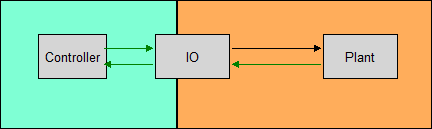
\includegraphics[width=0.5\linewidth]{controllerPattern/toplevel}
\end{subfigure}
\begin{subfigure}
\centering
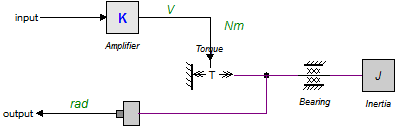
\includegraphics[width=0.45\linewidth]{controllerPattern/plant}
\end{subfigure}
\caption{The 20-sim top level model (left) and the plant (right)}
\label{fig:20simmotor}
\end{figure}

\section{Contract} The contract contains two variables of type
\keyw{real}. A monitored variable, \texttt{counts}, represents data
returned from the sensor monitoring the movement of the wheel, in the
form of a figure representing the number of radians rotated. A
controlled variable, \texttt{rev}, produces a output signal for the
motor actuator.

\section{Discrete-event} The DE model contains a
\texttt{Controller} class, which has the main thread of control.  The
\texttt{Control\-ler} instantiates abstract classes to represent the
actuator (\texttt{IActuatorReal}) and the sensor
(\texttt{ISensorReal}). At run-time concrete implementations of these
classes are provided by the \texttt{Actuator} class and the
\texttt{Sensor} class respectively. Designing a controller that
primarily handles abstract classes makes it easier to replace or alter
the concrete implementation at a later date if necessary.

The \texttt{Controller} is deployed onto a CPU running at 10MHz
by the \texttt{System} class.

\section{Continuous-time} There are two versions of the CT model
provided in 20-sim, one with all control implemented entirely in a CT
(20-sim) model, and one with all control implemented in VDM (i.e., a
\DESTECS co-model). Both models share the same plant, in which a power
signal, \emph{K}, is output to a motor, \emph{T}, which produces torque to rotate
a wheel, \emph{J}, modeling its inertia, whilst the bearing attached to the wheel models friction.

In the CT-only model the
\texttt{Controller} block houses the controller that calculates an
appropriate output for the motor. 

In the second model - a \DESTECS co-model - the
functionality previously implemented by the \texttt{Controller}
has now been moved into a VDM model in the \DESTECS tool, and so the second implementation of the 
\texttt{Controller} block, now takes responsibility for importing data to and exporting data
from the DE model. 

With two implementations available, the Simple Controller model
permits a modeller to experiment by locating different functionalities
in different parts of the model (for example, moving the controller
functionality from the CT model to the DE model) and comparing the
results. 

\section{Usage} 
The Simple Controller is a simple
example of a basic model. A good way to see how the model works
would be to run and compare the two versions (the CT-only and
the co-model). The CT-only model should be launched directly
from 20-sim. To do this, right click on the high-level \texttt{Controller} block in
20-sim, select \texttt{Edit Implementation}, and select
\texttt{CT}, and launch the model. 
Alternatively one can select \texttt{Destecs} here and
then launch the co-simulation from the \DESTECS tool.

\chapter{Water Tank (Periodic)} \label{chap:watertankperiodic}
\section{Case Description}
This model is an implementation of a water tank that is supplied by a
flow of water.  There is a valve at the bottom of the tank which can
be opened so that water flows out of the tank, or closed to stop the
exiting flow of water.  Underneath the tank we assume that there is a
drain to catch the outflowing water.  The tank is equipped with a
sensor to measure the current water level.

Figure \ref{fig:waterTank} illustrates the tank, the water flowing in,
the valve and the drain as components in a CT model, with a DE model
providing a controller.

\begin{figure}[!ht]
\centering
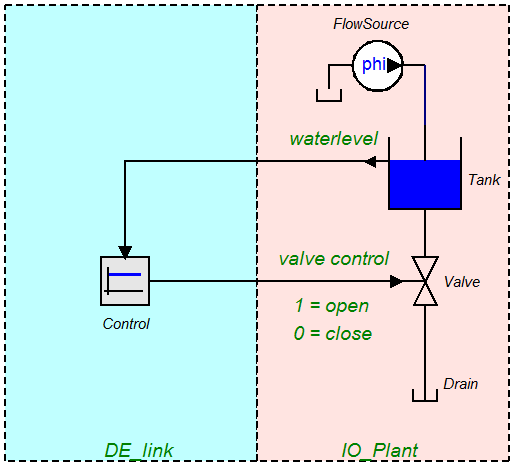
\includegraphics[width=7cm]{waterTankPeriodic/WaterTank.png}
\caption{Overview of the water tank in the case
  study \label{fig:waterTank}}
\end{figure}

We should like the water in the tank to remain between some maximum
and some minimum level.  If the water level falls below our minimum
desired level then the valve must be closed to ensure water stops
flowing out of the tank.  If the water rises above our maximum desired
level, then the valve must be opened to enable water to flow out.
This particular water tank model accomplishes this by polling the
water level sensor periodically, at intervals of \emph{n}
milliseconds, to monitor the current water level, checking that it
falls within acceptable boundaries, and taking some action if it does
not.

\section{Contract}
The contract for the periodic water tank model includes one
\emph{monitored} variable of type \keyw{real} (called \texttt{level})
which represents the current level of water measured by the sensor.
And there is one \emph{controlled} variable of type \keyw{bool}
(called \texttt{valve}) which is a signal to open or shut the valve.

In addition, there are two shared design parameters of type
\keyw{real}: \texttt{maxlevel} and \texttt{minlevel}, which dictate
the desired maximum and minimum level of the water respectively.  The
shared design parameters can be configured at runtime when executing a
simulation of the model, by opening the debug configuration options in
the DESTECS tool before the simulation is started.

\section{Discrete-event}
The DE model contains a \texttt{Controller} class, which has the main
thread of control.  An instance of \texttt{LevelSensor} is created to
represent the sensor that measures the current water level.  An
instance of \texttt{ValveActuator} is created to represent the valve
at the bottom of the tank.  \texttt{LevelSensor} simply returns a
value to represent the current level of water, whilst
\texttt{Valve\-Ac\-tu\-a\-tor} accepts a boolean value that sets the valve to
be open or closed.

The \texttt{Controller} starts a single thread that loops repeatedly,
waiting for some milliseconds \emph{n} and then collecting a reading
from the water level sensor.  If the level is calculated to be above
the desired maximum level then \texttt{Controller} sets the valve to
be open, calling the appropriate method in the \texttt{ValveActuator}
class.  Similarly, if the water level is calculated to be below the
desired minimum level then \texttt{Controller} sets the valve to be
closed.  The same thread continues to loop.

The \texttt{Controller} is deployed onto a single CPU
by the \texttt{System} class.

\section{Continuous-time}
The CT model for the periodic water tank consists of two main parts,
one to represent the link to the DE side of the model (\texttt{DE\_link})
and one to represent the CT side (\texttt{I\_O\_Plant}).

The \texttt{DE\_link} block handles interaction with the DE
model itself.  It contains a block, \texttt{Control}, which handles
the input from the DE model (\texttt{valve}, to represent a signal for
the valve actuator) and also the output from the CT model
(\texttt{level}, which represents the current water level as read by
the sensor).  These are the shared variables declared in the contract.

The \texttt{I\_O\_Plant} block incorporates other blocks to
represent the plant.  There is a \texttt{Flow\-Sour\-ce} to represent the
source of incoming water, a \texttt{tank} to contain the water and a
\texttt{Valve} at the bottom of the tank to control outward flow.
Underneath the tank is a \texttt{Drain}.

\section{Usage}
Running a simulation of the periodic water tank illustrates how
the water level in the tank rises until the maximum level is reached,
at which point the valve is opened and the level falls until the
minimum is reached.  The valve is then closed again and the process
repeats itself.  One way to experiment with the model is to change the
shared design parameters which dictate the values for the maximum and
minimum water levels.  These can be set in the Debug configuration
window in the DESTECS tool.  We recommend changing the values and
running the co-simulation with these varying values to view the effect
on the behaviour of the system.

\chapter{Water Tank (Event-Driven)} \label{chap:watertankeventdriven}
\section{Case Description}
The event driven water tank model is very similar to the periodic
water tank model described in Chapter \ref{chap:watertankperiodic}.
It models a water tank that is supplied by a flow of water inwards.
There is a valve at the bottom of the tank which can be opened so that
water flows out of the tank, or closed to stop the outflowing water.
Underneath the tank we assume that there is a drain to catch any water
flowing out.  The tank is equipped with a sensor to measure the
current water level.

We should like the water in the tank to remain between some maximum
and some minimum level.  If the water level falls below our minimum
desired level then the valve should be closed to stop the outflow.  On
the other hand, if the water rises above our maximum desired level,
then the valve should be opened to enable water to flow out.

The event-driven model accomplishes this using events, which are
triggered on the CT side of the co-model.  When the water level sensor
detects that the water is too high, it triggers a appropriate event
and signals the DE model.  The DE model then triggers the valve to
open by signalling the valve actuator.  Similarly, if the sensor
detects a water level that is too low, the CT model triggers a
different event and signals the DE model; the DE model then closes the
valve.

\section{Contract}
The contract for the event-driven water tank model is very similar to
that for the periodic water tank model.  It includes one
\emph{monitored} variable of type \keyw{real} (called \texttt{level})
which is the signal representing the current level of water in the
tank as measured by the sensor.  And there is one \emph{controlled}
variable of type \keyw{bool} (called \texttt{valve}) which is a signal
produced by the DE model to open or shut the valve.

In addition, there are two shared design parameters of type
\keyw{real}: \texttt{maxlevel} and \texttt{minlevel}.  The shared
design parameters can be configured at runtime when executing a
simulation of the model, by opening the debug configuration options in
the DESTECS tool before the simulation is started.

Finally, the event-driven model also includes two declared events:
\texttt{high}, which is an event triggered when the water level passes
some maximum desired level; and \texttt{minLevelReached}, which is
triggered when the water level falls below some desirable minimum
level.

\section{Discrete-event} The DE model contains an
\texttt{Controller} class, which has the main thread of control.  An
instance of \texttt{LevelSensor} is created to represent the sensor
that measures the current water level, and also an instance of
\texttt{ValveActuator} is created to represent the valve at the bottom
of the tank.  An instance of \texttt{WatertankEventHandler} is created
to receive the events that will be triggered by the CT model.

\texttt{LevelSensor} returns a value to represent the current level of
water, whilst \texttt{ValveActuator} accepts a boolean value that sets
the valve to be open or closed.  We assume that the level sensor is
able to self-detect and report some errors, and the
\texttt{LevelSensor} class checks for these. The class
\texttt{WatertankEventHandler} exists to catch the events triggered by
the CT model and react to them.  It reacts to the \texttt{high} event
by opening the valve on the tank, and it reacts to the
\texttt{minLevelReached} by closing the valve.

\section{Continuous-time}
The CT model for the periodic water tank consists of two main parts,
one to represent the link to the DE side of the model (\texttt{DE\_link})
and one to represent the continuous-time side
(\texttt{I\_O\_Plant}).

The \texttt{discrete-event} block handles interaction with the DE
model itself.  It contains a block, \texttt{Control}, which handles
the input parameter produced by the DE model and also the parameter
for data output by the CT model.  It also houses some logic for
triggering the relevant events.  Events in this case are triggered by
a zero value being reached.  The event \texttt{minLevelReached} is
used to communicate to the DE model that the water level has fallen
below some minimum desirable level of water, and is calculated by
subtracting the minimum desired level from the actual current level; a
result at zero results in the triggering of the event
\texttt{minLevelReached}.  Similarly, the maximum desired level is
also subtracted from the current level; when the result is zero this
triggers the event \texttt{high}.

The \texttt{continuous-time} block incorporates other blocks to
represent the plant.  There is a \texttt{FlowSource} to represent the
source of incoming water, a \texttt{tank} to contain the water and a
\texttt{Valve} at the bottom of the tank to control outward flow.
Underneath the tank is a \texttt{Drain}.

\section{Usage}
As with the periodic water tank model, running a simulation of the
event-driven water tank will illustrate how the water level in the
tank rises and falls between the maximum and minimum levels.  One way
to experiment with the model is to change the shared design parameters
which dictate these levels and experimenting to observe the effect on
the model's behaviour.  These can be set in the Debug configuration
window in the DESTECS tool.

\chapter{Paper Pinch} \label{chap:pidPinch}

\section{Case Description}
The paper pinch co-model illustrates a device for
manipulating paper (e.g., in a printer) and includes several
different types of fault modelling. A pair of rollers sit one
above the other and a motor is capable of rotating the
bottom-mounted one. The top roller is spring loaded to produce a
light downward pressure at all times. Rotating the bottom roller
allows the pair to `pinch' a sheet of paper and pass it between
the two rollers, thus moving it through the printer. An overview
of the rollers and motor and how they are connected can be seen
in Fig~\ref{fig:paperPinch}.

\begin{figure}[!ht] \centering
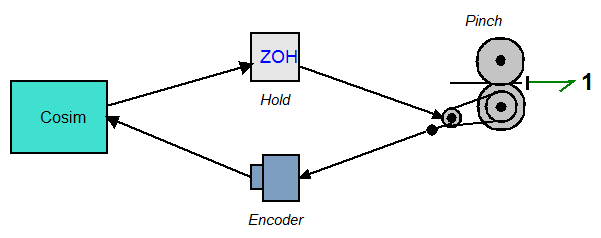
\includegraphics[width=0.7\textwidth]{pidPinch/pidPinch.png}
\caption{Diagram of a single pair of rollers in a printer
("Pinch"), the cosim Controller, an output line between
controller and pinch (with a zero-order hold) and an encoder to
feed data back to the Controller.} \label{fig:paperPinch}
\end{figure}

A real printer might typically have many sets of `pinches' to
manipulate the paper from an input tray through the printing
process to the output tray. This often involves moving the paper
in S-curves as well as in a simple linear direction. There is a
requirement that the pinches in the system move paper at a
synchronised speed. If one pinch feeds the paper too quickly or
too slowly to its neighbours then the paper will fold and bunch
up between the sets of pinches, or will be torn, and result in a
paper jam. Alternatively the paper may become skewed,
resulting in suboptimal print quality.

The main purpose of this co-model is to simulate some different
types of fault handling. The co-model allows the modelling of
two types of faults and two fault tolerant techniques.

\section{External Links}
The model was described in \cite{Pierce&11}.  This paper demonstrated
the modelling and simulation of errors and fault tolerance mechanisms
for embedded systems.

\section{Contract} The contract contains four shared state
variables of type \keyw{real}. One of these is responsible for
signalling power to the actuator \texttt{pwm}. This increases or
decreases the speed of the roller to control movement of the
paper through the pinch. Three more shared state variables are
used to read the current speed of the rollers, delivered by
three separate encoders: \texttt{enc1}, \texttt{enc2} and
\texttt{enc3}. %\begin{itemize} %\item Monitored variables
%\item Controlled variables %\item Shared design parameters
%\end{itemize}

\section{Discrete-event} The DE model implements a basic Decorator
pattern (as described by Gamma \emph{et al} \cite{gamma}), consisting
of the \texttt{Controller} which has the main thread of control, as
well as an \texttt{ISensorInt} abstract class to monitor the readings
from the pinch and an \texttt{IActuatorPWM} abstract class to produce
a power signal to the actuators. In the model \texttt{Encoder} is
provided as a possible implementation of the abstract
\texttt{ISensorInt}, and \texttt{PWM} is provided as a possible
implementation of the abstract \texttt{IActuatorPWM}.

The paper pinch model simulates several types of faults, and also
incorporates several methods for fault tolerance (see
Section~\ref{sec:CTpinch} for details of faults which are
injected). Firstly, the \texttt{Controller} is capable of implementing
a voting system, which helps to detect cases where a single encoder
has produced an incorrect value. This functionality is implemented in
the \texttt{Voter} class, which is an alternative implementation of
\texttt{ISensorInt}.  \texttt{Voter} considers inputs from multiple
sensors and translates this into a single value.

A further aspect of fault management is implemented in the
\texttt{SafetyKernel} class, which is an alternative implementation of
\texttt{IActuatorPWM}. \texttt{SafetyKernel} intercepts the
controller's output to the power line and caps the signal to some
absolute value.  This prevents sudden large increases or decreases in
power delivered to the actuator; if a mistake has been made and the
\texttt{Controller} produces an inappropriate power output to the
actuator, then this behaviour will curb the severity of the fault.

\section{Continuous-time} \label{sec:CTpinch}
The CT model includes a controller block (\texttt{Cosim}) which
handles the interface with the DE model. The controller produces a
power signal to an actuator, which then rotates the bottom roller in
the pinch device. Sensors detect the actual rotational speed achieved
by the pinch and several encoders feed this information back to the
controller.  The input to the encoder is the speed of some shaft in
revolutions per second and the output is a count indicating the number
of rotations.

The purpose of this co-model is to simulate fault handling and so the
co-model includes three encoders, to allow the model to simulate
different types of faults. Each encoder includes a fault block that
can intercept the input to the encoder and inject a possible
fault. One of the three encoders is fault-free, one produces
occasional bit-flips (sudden, large-value errors in the reading) and
the final encoder produces a `drift' error (low-value, cumulative,
gradual errors in the reading).  The fault blocks can be individually
triggered to inject a fault.

\section{Usage of fault tolerant features} The primary purpose of this model is to
simulate different types of fault and fault tolerance, and so one
obvious scenario is to test the fault handling.  As previously
described in Section \ref{sec:CTpinch}, there are three encoders, each
with a fault block.  By default, one fault block in this model is set
to produce a bit-flip error (characterised by a sudden large error in
the value read in); one is set to produce a `drift' type of error
(characterised by small, gradual errors); and one fault block is
configured to produce no error at all.  Running a simulation with the
default configuration will show output from all three encoders
alongside their respective fault blocks; a change in the signal for a
fault block indicates that it has activated and injected a fault into
the model.  There will be subsequent changes in other readings as the
model detects and copes with the change.  For example, when a bit-flip
fault is triggered, the output from \texttt{Encoder1} can be seen to
change value suddenly. If the model is employing the fault tolerant
\texttt{Voter} and \texttt{SafetyKernel} implementations of the
\texttt{ISensorInt} and \texttt{IActuatorPWM} classes, the
\texttt{Voter} class can cope with the bit flip by considering the
values of all three encoders and deciding that because the reading
from \texttt{Encoder1} does not correspond with the others it is a
fault and should be ignored; as a result the output value from the
\texttt{Controller} does not change.

\begin{figure}[!ht] \centering
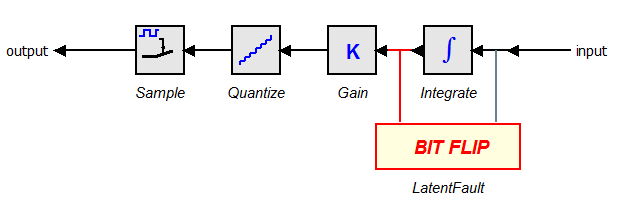
\includegraphics[width=0.7\textwidth]{pidPinch/pidPinchFaultBlock.png}
\caption{Diagram of the blocks inside an encoder for the paper pinch
  co-model, showing a fault block intercepting the input value.}
\label{fig:paperPinchFaultBlock}
\end{figure}

A good next step would be to configure the fault blocks.  Any of the
fault blocks can be set to produce a bit-flip fault, a bit-drift
fault, or no fault at all.  To to this, open the CT model in 20-sim
and double click on an encoder block to open it up.  Figure
\ref{fig:paperPinchFaultBlock} shows an encoder with a fault block
attached; the fault block, when triggered, tampers with the input
signal and produces an erroneous output.  To configure the fault
block, right-click on it and select "Edit Implementation".  This
produces a menu with "bitflip", "drift" and "nofault" as options.
Using this method, it's possible to change the type of error that is
produced for different encoders.  It's also possible to configure the
time in the simulation at which the fault block is triggered to
produce a fault.  To do this, right-click on the fault block and
select "Parameters" (click "yes" if 20-sim asks if it should check the
model first).  This produces a dialog box where parameters for the
fault block are set; changing the value for the "fault\_time"
parameter will change the time when the fault-block activates and
injects a fault during the simulation.  We recommend experimenting
with changing the types of error on each encoder, and changing the
times when faults are triggered, and then running the simulation to
examine how the model copes with different types of fault: i.e., how
quickly it can detect them and take some corrective action.



\chapter{Aircraft Fuel System}
\label{chap:fuelSystem}

\section{Case Description}

The fuel system on-board aircraft is a complex system where fuel must
be transferred between multiple tanks to ensure the engines always have
a sufficient supply of fuel and that the aircraft is in balance. An
overview of the fuel tanks and how they are connected can be seen in
Fig~\ref{fig:fuelTanks}.

\begin{figure}[!ht]
\centering
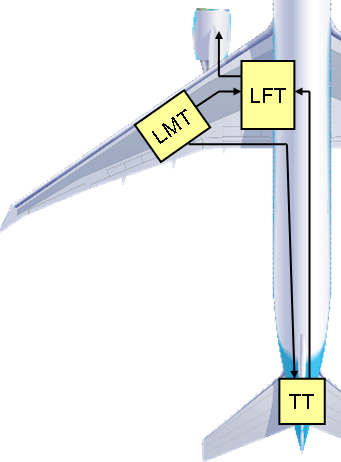
\includegraphics[width=4.5cm]{fuelSystem/FuelTanks.png}
\caption{Overview of the fuel tanks in the case
  study \label{fig:fuelTanks}}
\end{figure}

In the real system, tanks are also placed symmetrically in the
right-hand side of the aircraft --- these have been abstracted away in
the model.

At takeoff, the Trimmer Tank (TT) placed in the rear end of the
aircraft must be empty for safety reasons, but once cruise altitude
has been reached the trimmer tank must be filled to distribute weight
and therefore obtain better balance of the aircraft. The Left Feeder
Tank (LFT) must always have sufficient supply of fuel to the engine
which continuously consumes fuel (more during takeoff than at cruise
altitude). If the level of fuel in the feeder tank reaches a minimum
threshold fuel must be pumped from the Left Middle Tank (LMT) to the
feeder tank. If the middle tank becomes empty, fuel must be transferred
from the trimmer tank to ensure a sufficient level of fuel for the
engine. Finally, before landing the aircraft the trimmer tank must be
empties for safety reasons.

The purpose of the model was to model different faulty scenarios
(e.g.\ failing sensor) and examine if the aircraft had sufficient
fault-resilience mechanisms to ensure that the aircraft can land
safely.

%\begin{itemize}
%\item A short description of the system in the model
%\item Purpose of the model
%\item Assumptions/abstractions
%\item Key features ***
%\end{itemize}

\section{External Links}

The model was used in a comparative study~\cite{Wolff&12}, analysing
the collaborative modelling capabilities of the \DESTECS tool as well
as the Ptolemy tool~\cite{Buck&94,Davis&99,Eker&03}.

The aircraft fuel system case is inspired by the work of Jiminez et
al.~\cite{Jimenez&07} --- the \DESTECS model only includes the
left-hand side of the aircraft fuel system and the outermost tank is
removed. A similar case study modelled in Ptolemy is published
in~\cite{DerlerLeeSangiovanniVincentelli11_ModelingCyberPhysicalSystems}.

%\begin{itemize}
%\item Papers/technical reports where the model is used
%\end{itemize}

\section{Contract}

The contract contain three monitored variables of type \keyw{real}
used to read the current fuel level of the three tanks:
\texttt{LFT\_lvl}, \texttt{LMT\_lvl} and \texttt{TT\_lvl}. To control
the flow of fuel between the three tanks the DE controller uses the
following three controlled signals of type \keyw{bool} to pumps in the
system: \texttt{LMT2LFT\_valve}, \texttt{LMT2TT\_valve} and
\texttt{TT2LFT\_valve}. Finally, the contract contain two events used
to trigger state change in the controller: \texttt{enter\_cruise} is
triggered when the aircraft reaches cruise altitude, and
\texttt{enter\_pre\_landing} is triggered when the aircraft is close
to landing and the trimmer tank needs to be emptied.

%\begin{itemize}
%\item Monitored variables
%\item Controlled variables
%\item Shared design parameters
%\end{itemize}

\section{Discrete-event}

The DE model consist of the \texttt{Controller} which has the main
tread of control, as well as a \texttt{TTWatchdog} monitoring the
readings from the TT fuel level sensor (used for detecting faulty
readings). In addition, an abstract boolean actuator and the concrete
implementation \texttt{PumpSwitch\-\_CT} is also part of the
model. There are two abstract sensors (one for normative and faulty
behaviour) and a concrete implementation of both of these sensors.

The \texttt{Controller} and \texttt{TTWatchdog} are deployed on two
separate CPUs running at 10MHz which are connected by a single BUS.

%\begin{itemize}
%\item Overview (architecture)
%\item DE parameters (Architecture (CPU/BUS), Time (duration/cycles))
%\end{itemize}

\section{Continuous-time}

On the top level of the hierarchy, the model consists of three main
parts: I\_O, the plant and a block used for the 3D
animation. The I\_O handles the passing of variables to/from the
DE controller model. The animation block scales the level values from
the three tank between 0 and 1 to be used in the 3D animation. The
plant block contains the three tanks as well as the switches
controlling the flow between the tanks.

The three tanks are modelled identically, and only the max capacity
and the starting fuel level are different. The tanks themselves
ensures that the fuel level is always between the empty and full
thresholds, that the fuel can only enter the tank if it is not full,
and that fuel only can be pumped from the tank if it is not empty.

%\begin{itemize}
%\item Overview (hierarchy)
%\item CT parameters
%\end{itemize}

\section{Usage}

The fuel system model comes with a single scenario script used for
triggering the faulty TT level sensor:

\begin{dcl}[caption=DCL script activating the faulty trimmer tank level sensor.,label=list:dcl]
when time >= 3.9 do ( ct boolean TTLEVELERROR := true; );
\end{dcl}

Once the error is triggered in the CT model, the TT level sensor will
start sending a \emph{faulty value} of value 9e18 from the
\texttt{TT\_level\_Fault} block of the Plant in the CT model. A
\texttt{TTWatchdog} class monitors the readings from the trimmer tank,
and if two consecutive faulty values are read the asynchronous
operation \texttt{TTErrorDetected} in the \texttt{Controller} class of
the DE model is invoked and the fault is handled.

%\begin{lstlisting}
%parameters
%  boolean global TTLEVELERROR;
%
%equations
%  if(TTLEVELERROR) then
%    output = failvalue;
%  else
%    output = input;
%  end;
%\end{lstlisting}



%\begin{itemize}
%\item Change this param -> expected result
%\end{itemize}

%\chapter{Pacemaker} \label{chap:pacemaker}
\section{Case Description}
This model represents a pacemaker, which is a device surgically
implanted into patients at risk of certain life-threatening
irregularities developing in their heart.  A pacemaker has the task of
monitoring the heart's behaviour, and taking action if necessary to
ensure that a regular heart rate is maintained.

A human heart is divided into four chambers: at the top of the heart
are two smaller chambers: the left and right atria; and at the bottom
of the heart are two larger chambers: the left and right ventricles.
Each chamber is made of a wall of cardiac muscle fibres that contract
and then relax many times per minute.  The contractions force blood
currently inside the chamber outwards (via blood vessels).  The
subsequent relaxation of the muscle fibres allows more blood to
enter.  This maintains the regular movement of blood around the body,
and the rate and regularity with which the cardiac muscles contract
and expand is therefore very important for cardiac health.
\begin{figure}[!ht]
\centering
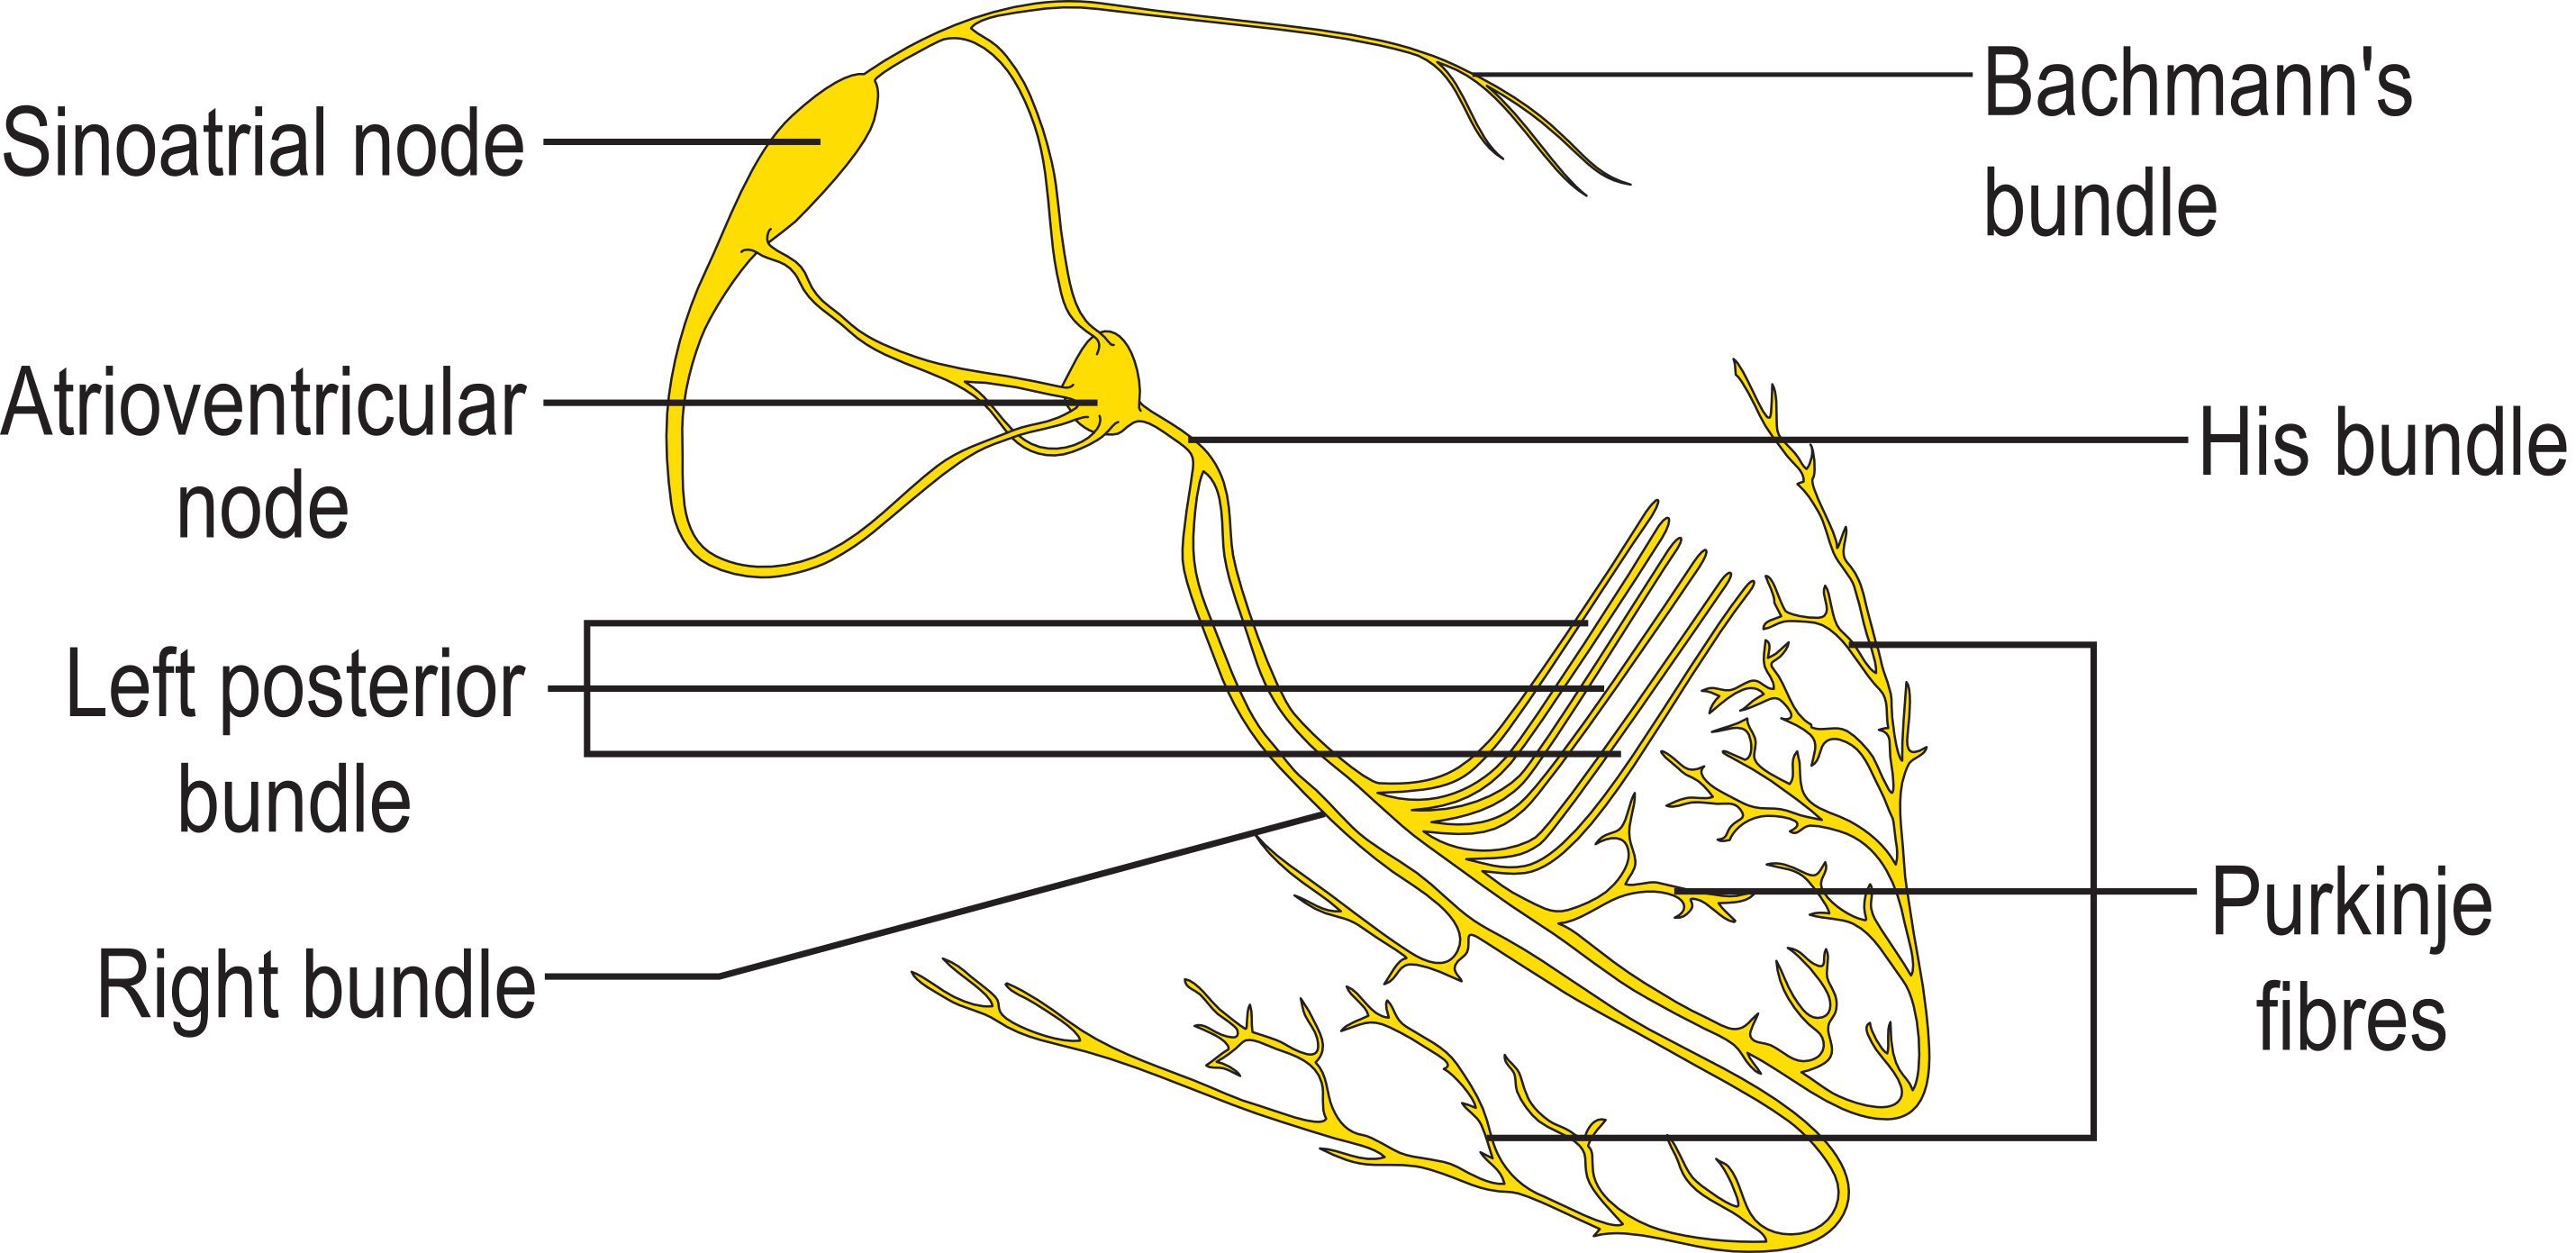
\includegraphics[width=8.5cm]{pacemaker/ConductionsystemoftheheartwithouttheHeart.png}
\caption{Electrical system of the heart.  Source:\\
  http://http://en.wikipedia.org/wiki/File:ConductionsystemoftheheartwithouttheHeart.png \label{fig:heart}}
\end{figure}

Figure \ref{fig:heart} shows the layout of the electrical system of
the heart.  The contraction of the cardiac muscle fibres is triggered
by an electrical discharge which is produced by a sinoatrial (SA)
node, situated above the atria, and by a second node, the
atrioventricular (AV) node, which is located between the atria and the
ventricles.  The two nodes are connected via a set of pathways.  A
healthy heart normally produces, in a single cycle, an electrical
discharge from the SA node, followed by a short pause, and a similar
discharge from the AV node.  This causes a regular pumping motion,
with the atria contracting and disgorging blood, then expanding just
in time to accept the blood being disgorged from the ventricles as
they contract in their turn.

A real heart is very complex and the co-model provided here
necessarily simplifies it.  In the DESTECS co-model, we represent the
heart's electrical system primarily as an SA node, an AV node and
pathways between them.  An electrical charge builds in the model
representation of the SA node over a period of time until it reaches a
threshold when it discharges quickly.  This discharge would be
absorbed into the muscle fibres surrounding the atria, and would cause
them to contract.  In the model the AV node also builds up an
electrical charge over a period of time; this charge includes some of
the charge communicated from the SA node via the pathways.  When the
AV node reaches its own threshold, it, too, discharges its electrical
charge.  This would cause the cardiac muscles in the walls of the
ventricles to contract in turn.

In a real heart, each of the two nodes has a natural rhythm for
discharging current.  The SA node tends to discharge approximately
70-100 times per minute in an average adult, and the AV node
approximately 40-60 times per minute.  In practice, however, the two
discharges in a healthy heart are synchronised and occur at the pace
dictated by the SA node.  In the co-model, this also happens; the
current discharged by the SA node is absorbed by the AV node, causing
it to reach its own discharge threshold more promptly that otherwise.

The pacemaker co-model implements a simplified version of the
behaviour of a healthy heart as described above, and also models two
well-known irregular behaviours, (there are many possible heart
irregularities we could model).  The two that we model are:

\begin{itemize}
\item \emph{Sino bradycardia}, a condition in which the SA node
  located at the top of the heart discharges too slowly.
\item \emph{Third degree atrioventricular block}, a condition in which
  the pathways connecting the two nodes fail to function properly.  Without communication between the nodes, the AV node tends to revert to
  its own, slower rhythm, and the atria and ventricles begin to lose
  their synchronisation.  The heart's efficient pumping action is thus
  compromised.
\end{itemize}

The pacemaker device has the task of monitoring the heart rate, and
when it detects that there is a problem it delivers an electrical
current to the cardiac muscle to force contractions at an appropriate
pace.  It does this only until the heart recovers and is able to
self-regulate once again, and so the pacemaker needs to monitor the
cardiac fibres continuously whilst delivering the necessary current to
regulate heart behaviour.  The pacemaker is usually connected to the
heart muscle by several electrical leads.  In this co-model, the
pacemaker itself is represented as a DE model, whilst the heart (i.e.,
the pacemaker's environment) is represented as a CT model.  The CT
model aims to model the electrical currents in the heart, and does not
model cardiac muscle fibres itself.

\section{External Links}
The pacemaker is described in the paper \cite{Gamble&12}, presented at
the Workshop on Trustworthy Cyber-Physical Systems.

\section{Contract} The contract for the pacemaker co-model contains
four variables of type \keyw{real}.  Two \emph{monitored} variables,
\texttt{atrial\_sensed} and \texttt{ventricular\_sensed}, represent
input from the sensor that detects whether the cardiac fibres in the
atria and the ventricles respectively have contracted.  And two
\emph{controlled} variables, \texttt{atrial\_paced} and
\texttt{ventricular\_paced}, deliver an electric current to the
cardiac fibres of the atria and the ventricles respectively, to force
them to contract.

\section{Discrete-event} The DE model contains a
\texttt{Controller} class which has the main thread of control.  The
\texttt{System} class creates a \texttt{Controller}, two instances of
the \texttt{ISensorReal} abstract class to represent the sensors which
monitor the cardiac muscle, and two instances of
\texttt{IActuatorReal} to represent the two leads that produce an
electric current for the muscle cells.  At runtime a concrete
implementation of the \texttt{ISensorReal} is provided by the
\texttt{Sensor} class, and a concrete implementation of
\texttt{IActuatorReal} is provided by \texttt{Actuator}.
\texttt{Actuator} simply handles the passing of a signal to the CT
model's actuators, and \texttt{Sensor} simply handles obtaining a
value from the sensors in the CT model.

The pacemaker needs to keep track of time elapsing in order to
determine if there are irregularities in the heart rate.  In the
co-model, the \texttt{Controller} class creates an instance of
\texttt{Data} to store this information.  In turn, \texttt{Data}
creates four instances of \texttt{Timer}, which is a class that has a
notion of tracking and measuring time passing.  These four instances
of \texttt{Timer} are used by the \texttt{Data} class to keep track
of: the interval since the atria last contracted; the interval since
the ventricles last contracted; the interval between the atrial and
ventricular contraction (there is normally a short delay between the
two contractions in a healthy heart); and the interval between
pacemaker interventions.  A \texttt{Parameters} class acts as a
configuration class and lookup table, storing global variables such as
the acceptable time to elapse between contractions.

\texttt{Controller} creates an instance of \texttt{Data}, which in
turn stores an instance of \texttt{Parameters} and initiates all the
timers.  The \texttt{Controller} class regularly checks the timers,
looking for timers that have expired.  An intervention is triggered if
a timer expires and we have not seen the associated expected event.
For example, we expect to see the ventricle fibres contract before the
timer assigned to measure the intervals between ventricular
contractions expires.  In this case a large signal is delivered to the
appropriate actuator to deliver an electrical current and trigger a
contraction of the ventricular muscles manually.

\section{Continuous-time}
The CT model consists of three main blocks: \texttt{SA Node} which
represents the sinoatrial node; \texttt{AV Node} which models the
atrioventricular node; and \texttt{Internodal Pathway}, which models
the pathways between them.  For modelling purposes, the CT presents a
simplification of the behaviour of the two nodes, assuming that they
build an electrical charge and then discharge it, in a fashion similar
to a capacitor.  This is a simplification of actual heart behaviour.

The \texttt{SA Node} includes a constant supply of positive electrical
charge (\texttt{Primary rate}) which accumulates in the block
\texttt{Atrial\_Store}.  This in turn feeds into the block
\texttt{Discharge Condition}, which dictates when the
\texttt{Atrial\_Store} should discharge its accumulated charge.  In
practice, this occurs once a certain threshold has been reached, and
because of the constant supply, at regular intervals.  An additional
block, \texttt{SB\_Fault}, can be configured to interfere with this
model if we wish to illustrate the behaviour caused by \emph{sino
  bradycardia}.  If this is the case, then the \texttt{SB\_Fault}
block tampers with the constant supply of electrical charge
(multiplying by a number below 1) in order to trigger discharges by
the SA node at inappropriately slow intervals.

The \texttt{AV Node} block is very similar to the \texttt{SA Node},
including a constant supply of positive electrical charge (from
\texttt{Secondary\_rate}), a store in which the charge accumulates
(\texttt{Ventricular\_Store}) and a block that dictates when the store
should discharge current (\texttt{Discharge Condition}).

The \texttt{Internodal Pathway} block accepts input from the
\texttt{SA Node} and produces output for the \texttt{AV Node}, to
represent the flow of charge from the SA node in a real heart to the
AV node.  It contains a single block, \texttt{AV\_Block}, which simply
exists to handle transfer of charge in one direction from \texttt{SA
  Node} to \texttt{AV Node}.  When the model is configured to model a
\emph{third degree atrioventricular block}, the charge is simply
blocked here and not passed between the two nodes.

There is a single additional block, \texttt{Pacemaker}, which acts as
the interface between the DE and CT models.  This block accepts inputs
from the DE model to represent electrical signals to trigger a
contraction, and provides outputs for the DE model to monitor whether
the cardiac muscle is contracting.  The input signals for the
\texttt{Pacemaker} are collected from the relevant nodes; the
\texttt{Pacemaker} examines the signal after the
\texttt{Atrial\_Store} or after the \texttt{Ventricular\_Store}, which
allows it to monitor whether the discharge condition is being met.


\section{Usage}
This co-model is best understood in the first instance by running it
with a healthy heart scenario.  A simulation of the co-model should
demonstrate contractions detected repeatedly firstly in the atria, and
then secondly in the ventricles.  There should be no output produced
from the pacemaker.

Next, different irregularities can be modelled by enabling them in the
CT model.  \texttt{fault1} can be set to {\textbf\ttfamily{true}} to
model the condition \emph{sino bradycardia} (where the SA node
discharges too slowly).  In this scenario, a simulation should show
that the expected event (contraction of the atria) is not detected by
the pacemaker, and so the pacemaker delivers a large current via the
shared variable \texttt{atrial\_paced} in order to trigger the atria
to contract.

To model the heart condition \emph{third degree atrioventricular
  block} (where the pathways fail to carry a charge between the nodes)
the global variable \texttt{fault2} should be set to
{\textbf\ttfamily{true}}.  In this case, a simulation of the co-model
should show that the pacemaker can detect a contraction in the atria,
but not in the ventricles.  Thus, after the atria have contracted and
a suitable short pause has elapsed, the pacemaker should deliver a
charge to the ventricles to force a ventricular contraction.

\chapter{Morse Code Reader} \label{chap:morsecodereader}
\section{Case Description}
This model represents a device for decoding a message presented in
Morse code.  Morse code is a system which uses one or more ``dots''
and ``dashes'' to represent standard Latin characters.  The dots and
dashes can be represented as long or short flashes of light, as long
and short audible tones, or as long and short marks on paper.  In this
case the message to be decoded is delivered as long and short marks on
a strip of light-coloured tape.  The marks represent dots if they are
narrow and dashes if they are wide.  The decoder has a sensor able to
detect light and dark on the tape and a motor which is capable of
moving the tape so that it passes in front of the sensor.  When it is
ready to read a message, the decoder produces a signal to the motor to
move the tape continuously past the sensor, and periodically collects
a reading from the sensor which indicates whether a light or a dark
colour is currently visible on the tape.  These readings are collected
and used to determined whether the tape is currently displaying a dot,
a dash or a space.  Information on dots and dashes and the spaces
between them is collected in turn, and then translated into standard
Latin characters using a lookup table.  Figure \ref{fig:morsereader}
presents a diagram of the Morse decoder device, showing the tape with
the message, the motor that moves the tape, the sensor to read the
tape and the controller which is linked to both sensor and motor.

\begin{figure}[!ht]
\centering
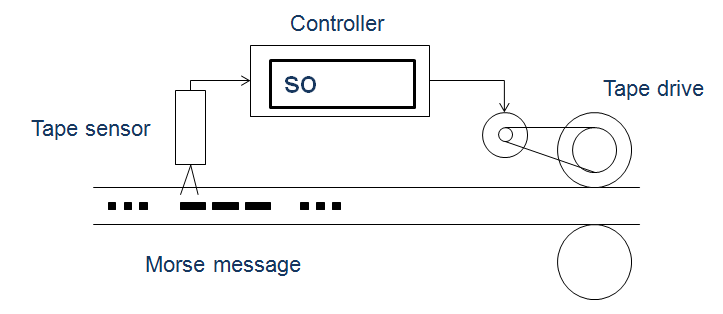
\includegraphics[width=8cm]{morseCodeReader/MorseTapeReader.png}
\caption{Overview of the Morse decoder \label{fig:morsereader}}
\end{figure} 

It's assumed that the message which is encoded is preceded by a
standard Morse ``attention'' sequence and is followed after its
completion by a standard ``end of work'' sequence.  The following
assumptions are also made:
\begin{itemize}
\item a dash is three times the length of a dot
\item there is a space (no signal) the same length as a dot between
  dots and/or dashes
\item there is a space the length of three dots between two separate
  ASCII characters
\item that there is space the length of seven dots between two ASCII
  words
\end{itemize}
The exact length of the mark used to represent a dot and the mark used
to represent a dash are unknown and must be calculated by the decoder
before message can be decrypted.  Therefore the Morse code reader
firstly detects the ``attention'' sequence that precedes the message,
and from this it performs some calibration to determine the width of a
dot and the width of a dash. The width is determined in terms of the
number of samples taken which were not background colour.

\section{Contract} The contract for the Morse decoder model contains two variables of type
\keyw{real}. A \emph{monitored} variable, \texttt{morseSensorShared},
represents input from the sensor that detects light and dark.  A
\emph{controlled} variable, \texttt{motorVoltageShared}, is used to
produce a signal to the motor which moves the tape past the sensor.

The contract also includes two shared design parameters of type
\keyw{real}: \texttt{AToDResolutionBits} and \texttt{AToDNoiseBits}.
These are used for configuring the noise and resolution of the input
data so that fault tolerance mechanisms may be exercised.

\section{Discrete-event} The DE model contains an
\texttt{AbstractMorseReader} class, which assumes the role of a
controller and has the main thread of control.  At runtime a concrete
implementation of the \texttt{Abstract\-MorseReader} is provided by the
\texttt{ModalController}, which in turn instantiates abstract classes
to represent the actuator for the motor
(\texttt{AbstractActuatorReal}) and the sensor
(\texttt{AbstractFilteredSensorReal}). At run-time concrete
implementations of these classes are provided by the
\texttt{ActuatorReal} class and the \texttt{FilteredSensorReal} class
respectively. Designing a controller that primarily handles abstract
classes makes it easier to replace or alter the concrete
implementation at a later date if necessary.

\texttt{ActuatorReal} allows the DE model to set the voltage for the
motor to move tape past the sensor.  \texttt{FilteredSensorReal}
allows the sample size to be set (how many samples are used to
determine if something is black or white, determined during
calibration), as well as reading in a value from the sensor.

Some other classes are also provided.  The \texttt{MorseLookup} class
provides a method to translate a sequence of dots and dashes into
ASCII characters.  The \texttt{DotDashOrSpace} provides methods to
check for the existence of a dot, a dash or a space given some input
from the sensor.

The process of decoding the Morse message involves a number of
different stages, or modes, of operation.  The
\texttt{ModalController} class stores a variable,
\texttt{controllerMode}, which is of type
\texttt{AbstractControllerMode} and is responsible for providing the
methods to be employed during the current mode.  During initial
operation \texttt{ControllerModeMeasureSignalNoise} provides the
concrete implementation of \texttt{AbstractControllerMode}; this class
examines the input whilst the tape remains stationary, in order to
determine the signal to noise ratio.  A higher level of noise results
in a lower overall speed being selected for reading the rest of the
tape.  The motor is off during this calibration phase but on for all
other phases.  Next the concrete implementation of
\texttt{AbstractControllerMode} is replaced with the
\texttt{ControllerModeMeasureDotDash\-Length} class, which provides
methods to handle the calibration process of identifying the attention
sequence and measuring dot length.  Then the mode changes again and
the functionality of the \texttt{AbstractControllerMode} is provided
by the concrete implementation \texttt{ControllerMode\-ReadMessage}.
This mode class provides methods to collect sensor readings at
appropriate sampling intervals and to translate collections of dots
and dashes.  Finally the concrete implementation is provided by
\texttt{ControllerModeIdle}, which simply ensures that the motor
voltage is set to zero.

The \texttt{AbstractMorseReader} (the controller class) is deployed
onto a single CPU by the \texttt{System} class.

\section{Continuous-time} 
The CT model consists of three main blocks, \texttt{controller},
\texttt{Motor} and \texttt{morseSensor}, in addition to a single block
which represents the plant. The \texttt{Controller} block handles the
interface between the CT model and the DE model. The \texttt{Motor}
block resides between the \texttt{Controller} and the plant, and
accepts an input which is the voltage to be applied to the motor
itself.

The \texttt{morseSensor} block represents the sensor and accepts some
input from the plant, handles A/D conversion and produces an output
for the \texttt{Controller}.  The output indicates how dark was the
currently visible section of tape.

\section{Usage} 
The model uses some data files to represent tapes with Morse code
messages, and some examples are provided with the model.  Each message
is represented in three files: an image is provided purely for the
user to visualise what the sensor should be able to see; a file
\emph{message.txt} represents the same data, but is actually used by
the sensor to generate data; and a further file
\emph{message-length.txt} is used to ensure that the image is
displayed to scale.  One way to get started with the model is to try
decoding different messages.  This simply involves running the model
with the included sample messages.  A further step could be to
generate your own message files and test out the decoding process. A
Java \emph{.jar} file, \texttt{TextToMorseTape.jar}, is included
alongside a readme file alongside the CT model.  This jar file can be
used to generate the three message files required, given some text.

The model needs to deal with the difficulty of reading a signal which
is delivered against some background noise.  The model copes with this
by analysing the signal-to-noise ratio before it begins and setting a
lower speed for reading more ``noisy'' data.  This allows the decoder
to take more samples for each of the dot or dash characters,
increasing confidence that data is accurately interpreted.  An
interesting experiment for the Morse decoder model involves varying
the amount of background noise that it is expected to cope with.  This
is set as a shared design parameter in the contract, and can be set at
runtime by opening the Debug configuration for the \DESTECS model.
Running the model with the same input files and higher levels of
background noise should see a slower decryption process because the
tape moves more slowly and more samples are collected, whilst
decreasing the background noise should see the decoder produce the
decrypted message more quickly.

\chapter{Line Following Robot} \label{chap:lineFollowingRobot}
\section{Case Description} The line following robot is a
co-model that demonstrates how design space exploration is supported
in DESTECS.  The co-model simulates a robot that can follow a line
painted on the ground. It is assumed that the colour of the line is
known and that it is differentiated from the background colour (which
is not known), but the line may exhibit gentle or sharp corners or
angled corners in any direction. The robot uses a number of sensors to
detect light and dark areas on the ground and has two wheels, each
powered individually with motors to enable the robot to make
fine-graded changes in direction.

\begin{figure}[htb!]
\begin{center}
\subfigure[An R2-G2P robot]
{
      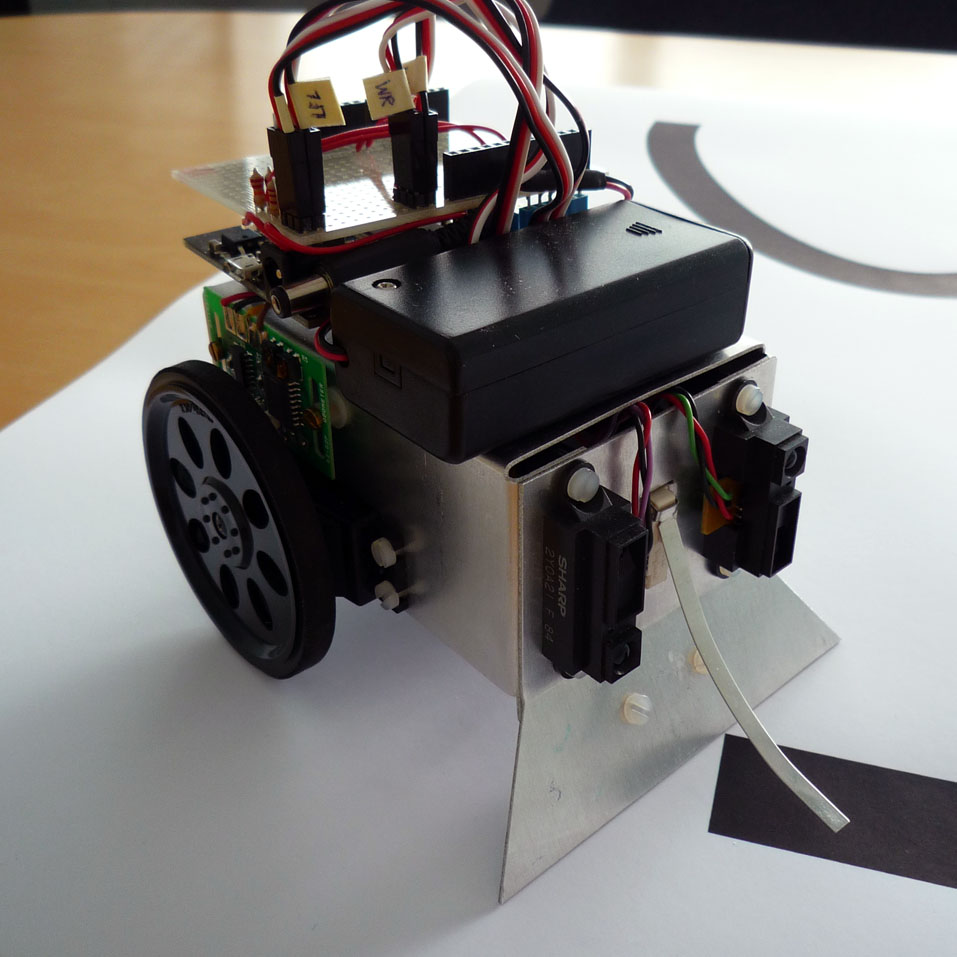
\includegraphics[width=0.3\linewidth]{lineFollowingRobot/r2g2p_netduino}
      \label{fig:r2g2p_sm}
}
\subfigure[A line-follow path]
{
      
\includegraphics[width=0.3\linewidth]{lineFollowingRobot/map}
      \label{fig:r2g2p_3dpath}
}
\subfigure[3D representation of the R2-G2P]
{
      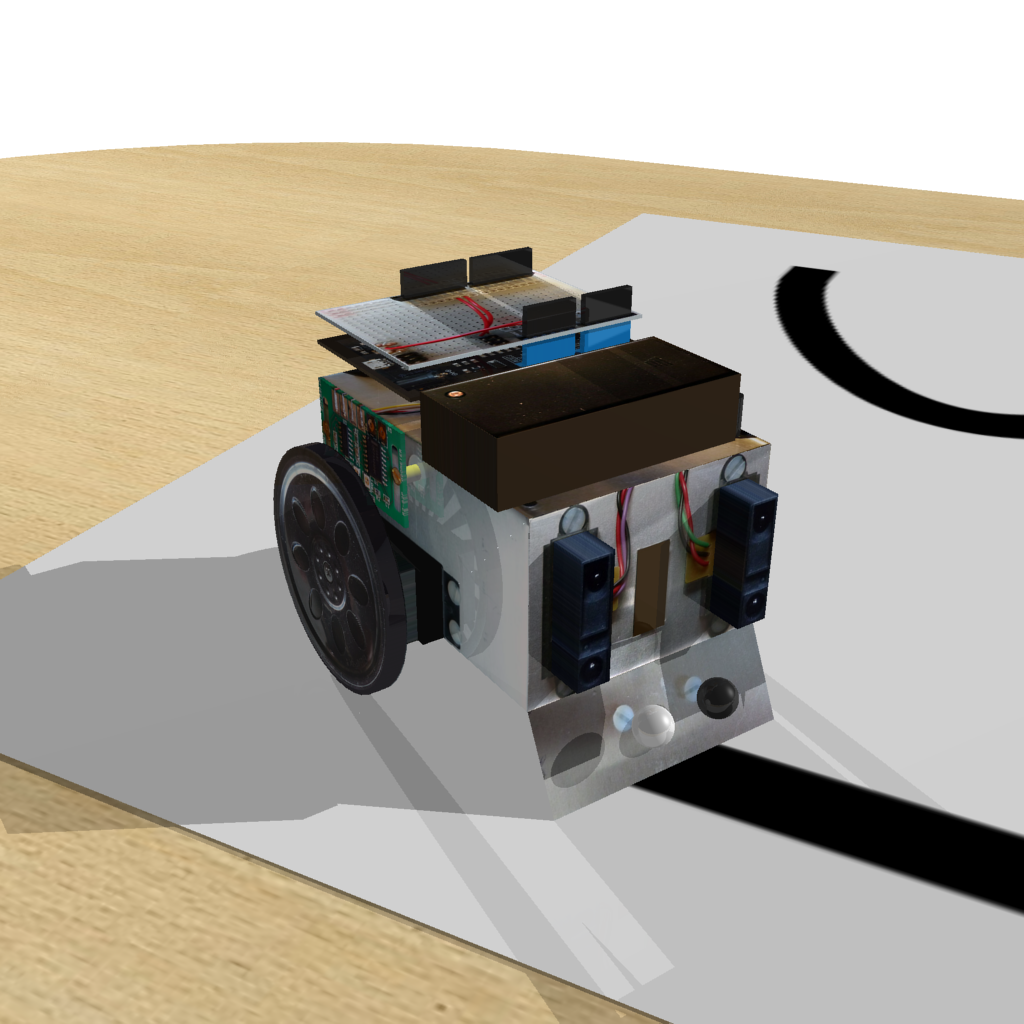
\includegraphics[width=0.3\linewidth]{lineFollowingRobot/robot_inside}
      \label{fig:r2g2p_3d}
}
\caption{The line-following robot}
\label{fig:r2g2p_study}
\end{center}
\end{figure}

There are a number of design decisions to make when designing the
robot.  For example, possible variations might include changing the
number of sensors or changing their positions (sensor position can be
adjusted laterally or longitudinally). Any given design can be
assessed by comparing distance travelled, which will be shorter for
more accurate robots, and average speed, which will ideally be as high
as possible.  DESTECS facilitates exploration of the design space by
automating simulations with different design parameters. For example,
DESTECS can automatically simulate a model with two sensors set
initially close together, then increasing the distance between them by
some distance \texttt{n} until a maximum distance is reached.  The
results of each simulation can then be compared to determine the ideal
robot design.

The co-model supplied here uses two sensors to detect light and dark,
and two motors (one for each wheel).  Two encoders (also one for each
wheel) close the feedback loop so that actual wheel rotations can be
monitored and the output to the motors adjusted accordingly.

The robot moves through a number of phases as it follows a line.  At
the start of each line is a specific pattern that will be known in
advance.  Once a genuine line is detected on the ground, the robot
follows it until it detects that the end of the line has been reached,
when it should go to an idle state.  For modelling purposes the
co-model accepts a textual representation of a bitmap as the surface with a line to be followed.

%\fbox{Can we insert a figure here?}
%\section{External links}


%-- shared design parameters
%sdp real wheel_radius;
%sdp real encoder_resolution;
%sdp real line_follow_x;
%sdp real line_follow_y;
%sdp array initial_position[3];
%sdp real fast_wheel_speed;
%sdp real slow_wheel_ratio;
%
%-- encoders
%monitored real encoder_left;
%monitored real encoder_right;
%
%-- line-following sensors
%monitored real lf_left;
%monitored real lf_right;
%
%-- line-following sensor fail flags
%monitored bool lf_left_fail_flag;
%monitored bool lf_right_fail_flag;
%
%-- servos
%controlled real servo_left;
%controlled real servo_right;

\section{Contract}
The contract contains eight shared variables.  Two \emph{controlled}
variables of type \keyw{real} produce signals for the actuators that
power the motors for the left (\texttt{servo\_left}) and right
(\texttt{servo\_right}) wheels.  And two \emph{monitored}
variables of type \keyw{real} are used to feed back information about
the rotations of the left (\texttt{encoder\_left}) and right
(\texttt{encoder\_right}) wheels.

Two \emph{monitored} variables of type \keyw{real} are used to represent
inputs from line-following sensors that can detect areas of light and
dark on the ground.  In this model there are two sensors,
\texttt{lf\_left} and \texttt{lf\_right}, but other models may carry more
or fewer line-following sensors.

Two \emph{monitored} variables of type \keyw{bool} are used to indicate
 whether a fault has been detected on the left wheel
 (\texttt{lf\_left\_fail\_flag}) or right wheel
 (\texttt{lf\_right\_fail\_flag}).  It is assumed that the CT model can
 self-detect and report some faults to the DE model.

%And finally, a single \emph{controlled} variable of type \keyw{matrix} is
%contained in the contract to represent an array of LEDs \texttt{leds}.
%The LEDs could be used to indicate the current state of the controller
%visually (e.g., in a 3D visualisation).

The contract also includes seven \emph{shared design parameters}: wheel radius, in metres (\texttt{wheel\_\-radius})); encoder resolution, in counts per revolution (\texttt{encoder\_resolution}); the separation of the line-following sensors from the centre line, in metres (\texttt{line\_follow\_x}); distance forward of the line-following sensors from the centre of the robot, in metres (\texttt{line\_follow\_y}); an array giving initial position \texttt{x}, \texttt{y}, \texttt{theta} (\texttt{initial\_position[3]}); and two shared variables representing controller aggression in terms of maximum wheel speed (\texttt{fast\_wheel\_speed}) and turn ratio (\texttt{slow\_wheel\_ration}), both in the range [0,1].

\section{Discrete-event}

The DE model makes heavy use of inheritance, providing abstract
classes for controller, sensors and actuators. The servos are accessed through objects of the \texttt{SpeedServo} class, which inherits from the \texttt{IActuatorRealPercent}; and the encoders are read through objects of the \texttt{Encoder} class, which inherits from the \texttt{ISensorReal}.

The line-following sensors make greater use of the benefits of inheritance. The raw sensor readings are accessed through objects of the \texttt{IRSensor} class, which inherits from the \texttt{ISensorInt8} class. Because the CT model of the line-following sensors includes sensor noise, the \texttt{Filtered\-IR\-Sensor} is used. This class contains an \texttt{IRSensor} and maintains a floating average using the last five sensor readings. This class also inherits from the \texttt{ISensorInt8}, which means that an \texttt{IRSensor} object can be swapped for a filtered object seamlessly. This is an example of the standard \emph{decorator} pattern~\cite{DESIGNPAT95}.

As mentioned above, the sensors are calibrated to set when it is considered to be reading black. This can change if the ambient light is increased in the model. The calibration is set in a \texttt{BlackWhiteSensor} class, which holds an \texttt{IRSensor} object and has Boolean operations to determine if the sensor is seeing black or white.

The controller is modal, meaning that with each `phase' (initialisation, sensor calibration, line-following, etc.) is realised as a mode, represented by the \texttt{IMode} interface. This interface defines four operations: \texttt{Enter}, called when the controller changes to this mode; \texttt{Step()}, called each control cycle; \texttt{Exit()}, called when the controller finishes this mode; and \texttt{Done()}, which allows a mode to indicate it has finished its task. The two abstract classes \texttt{AbstractMode} and \texttt{AbstractModeTimed} provide empty implementations of these operations. The timed mode keeps track of how long it has been running, and \texttt{Done()} will yield \texttt{\textbf{true}} after a specified time.

The top-level controller class is the \texttt{AbstractModalController}. This class holds a reference to each sensor object and provides getter methods to access these objects. The abstract mode classes hold a reference to the \texttt{AbstractModalController}, so that each mode can access the sensors and actuators. The \texttt{LineFollower} class is a subclass of this class, which instantiates the modes it requires to follow the line, which are held in a map. The identifier of the current mode is recorded in the \texttt{mode} variable and modes are changed with the \texttt{ChangeMode} operation. The \texttt{CheckModeChange} operation contains the logic for changing mode.

The following modes are followed in order: \texttt{WaitMode}, which gives the sensors time to start up; \texttt{CalibrateMode}, which calibrates the sensors using the predetermined starting pattern; \texttt{FindLineMode}, which drives forward until the line is found; and finally \texttt{FollowMode}, which follows the line.

If one of the sensors fails, the controller switched to  \texttt{SingleFollowMode}, which uses the one remaining working sensor to follow the line. Modes can also cause a change of mode by returning the identifier of a mode from the \texttt{Step()} operation. This functionality is used by the \texttt{SingleFollowMode} class to switch to \texttt{RefindLineMode} when it loses the line. The \texttt{RefindLineMode} sweeps back and forth until it sees black, then returns to \texttt{Single\-Follow\-Mode}.

The \texttt{System} class instantiates the
\texttt{LineFollower} object and deploys it to a single CPU. All sensor and actuator objects are created in the \texttt{IOFactory} class, which provides so-called ``factory'' methods that return the requested sensors. The \texttt{IOFactory} object is created in the \texttt{System} class and passed to the \texttt{LineFollower} object. The periodic thread is defined in the \texttt{Thread} class. This class holds a reference the controller and IO factory. This means that all the sensors and actuators can be synchronised at once, then the controller is called. This improves simulation speed.



\section{Continuous-time}

The CT model (pictured in Figure~\ref{fig:r2g2p_study}) is broken down into blocks that broadly represent physical components. The central \emph{body} block is a bond graph representation of the physics, with bond graph models of the wheels (\emph{wheel\_left, wheel\_right}) and servos (\emph{servo\_left, servo\_right}) connected on either side. The encoder blocks (\emph{encoder\_left, encoder\_right}) produce 44 counts per revolution of the wheel. Two line-following sensor blocks (\emph{lf\_left}, \emph{lf\_right}) are also connected to the body, as well a \emph{map} block. The encoder, line-following sensor and servo blocks are all connected to a \emph{controller} block that handles exchange of data with the DE model.

\begin{figure}[htb!]
\begin{center}
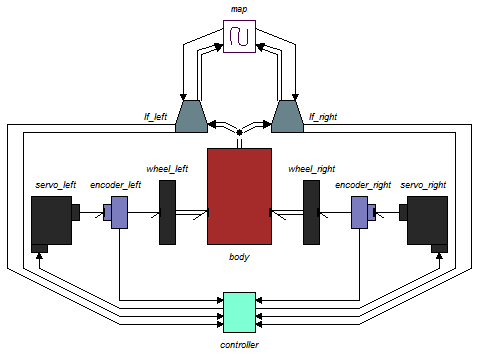
\includegraphics[width=0.6\textwidth]{lineFollowingRobot/r2g2p_ct}
\end{center}
\caption{Continuous-time model of the R2-G2P}
\label{fig:r2g2p_studyCT}
\end{figure}

The line-following sensor (seen at the top of Figure~\ref{fig:r2g2p_studyCT}) take the position and orientation from the \emph{body} block and calculate their position in the world using the \texttt{line\_follow\_x} and \texttt{line\_follow\_y} shared design parameters. This position information is passed to the map block, which takes a sample of values and passes a raw reading back to the sensors. The sensors then convert this to an 8-bit value, taking into account realistic behaviours: ambient light levels, a delayed response to changes, and A/D conversion noise.

The line-following sensor blocks also include a block to model a ``stuck'' failure (\emph{stuck\_fault}). This block has two implementations: the default (\emph{no\_fault}) does nothing to the signal and has an empty icon. The alternative is called (\emph{fail\_fixed\_value}) and has a thick, red outline and causes the sensor to always yield a fixed value (the stuck values are defined in the \emph{globals} block).

If the \emph{fail\_fixed\_value} implementation is selected in the left sensor, then it will fail after 12 seconds, always yielding 0 (black). If the \emph{fail\_fixed\_value} implementation is selected in the right sensor, it will fail when the value \texttt{lf\_right\_stuck\_value} is changed from -1 to a value between 0 and 255 by a script. The sensor will then yield whatever value is set, so this sensor can be made to get stuck on white, for example.


\section{Usage}

The line-following robot model is a good opportunity to see how
DESTECS can support design space exploration.  A good starting point
is to run the co-model (using the \texttt{LineFollowingRobot} launch configuration), examining the speed and accuracy (distance)
with which it can complete various lines. You can then run the \texttt{LineFollowingRobot\_Outside} launch, in which the shared design parameter \texttt{line\_follow\_x} has been increased so that the sensors are ``outside'' the line on either side. Note how the simple line-following algorithm still works.

Next you can try your own combinations by altering \texttt{line\_follow\_x} and \texttt{line\_follow\_y} and observing the results. The robot generally needs to be able to distinguish when it has encountered the end of the line, and when it has encountered a sharp angle that may take the line behind its
current field of view.  Changing the forward/back position of the
sensors may make this task easier or more difficult, whilst changing
the width between the two sensors also has an impact, by altering the
resolution of the information which can be gathered about the line.

To try various designs automatically, you can define an ``ACA Launch'' configuration. Select \texttt{LineFollowingRobot} as the ``Base Configuration'', then on the ``SDPs Sweep'' tab, then try the following values: \texttt{line\_follow\_x} from 0.01 to 0.05 by 0.02, and \texttt{line\_follow\_y} from 0.01 to 0.13 by 0.06. The DESTECS tool will then run 9 co-simulations generated from the above numbers.

Beyond this step, you could try to improve the robot's line-following. First, you could change \texttt{fast\_wheel\_speed} and \texttt{slow\_wheel\_ratio} (between 0.0 and 1.0) to alter the controller aggression. The robot could be made to drive more smoothly if a \emph{proportional} control mode was used, which applies more or less turn depending on how far from the line it is. You could change the \texttt{FollowMode} class, or create you own class and instantiate it in the constructor of \texttt{LineFollower} class.

Increasing the number of sensors would also allow for performance improvements. You can duplicate a sensor in the CT model and connect it up. You would need to alter the \emph{map} and \emph{controller} blocks to handle the new signals; instantiate more sensor objects in the DE model and make them accessible to the modes; and add a new entry to the contract / \texttt{vdm.link} file. Chapter \ref{chap:summerschoolmodels} describes five
different models of a similar line-following robot, each exhibiting
different design choices in terms of number and position of sensors,
as well as different methods for identifying the line against a
undetermined background.

\chapter{DESTECS Summer School models} \label{chap:summerschoolmodels}

\section{Introduction}\label{chap:summerschoolintro}
In July 2012 the DESTECS project hosted a summer school for
postgraduate level students and practitioners, which included
multi-day projects in groups.  Five groups in total were set the
assignment of developing their own line-following robots, including
setting appropriate design priorities and testing out different
possible designs to achieve the optimum result.  We include these
models here, as they provide a good demonstration of how DESTECS can
facilitate the exploration of the design space.  These models are
provided as-is, showing the real work of first-time DESTECS users
working on a time-limited project, and should be viewed as such. Photos of each group, along with their designs, are shown in Figure~\ref{fig:groupphotos}.

Each group had the same brief: to develop a line-following robot model
as described in Chapter \ref{chap:lineFollowingRobot}.  Groups aimed
to create the `best' performing robot, where performance was measured
by total time taken to follow a given set of lines (not known in
advance) and how accurately the robot measured these lines.  Models
were required to measure the time taken and the distance of the line
for this reason.  It is assumed that the robot has a fixed starting
position which begins with a predictable pattern on the ground before
the line begins.

As described briefly in Chapter \ref{chap:lineFollowingRobot}, there
are several design aspects to consider:
\begin{itemize}
\item There was no limit on the number of sensors that could be added,
  and there was considerable possibility for groups to experiment with
  this.  Whilst it is possible to design a robot with only one sensor
  that would fulfil the requirements of the exercise, adding more
  sensors may allow the robot to plot a more accurate course.
\item Groups were free to change the position of the sensors as they
  saw fit.  A particular problem is posed by the difficulty of
  detecting sharp, acute angles, resulting in the line doubling
  sharply back on itself.  Some designs of robot will find these
  scenarios difficult to detect and will lose track of the line's
  location.  This can be made easier or more difficult by placing
  sensors further forward, further back, wider apart or closer
  together, and several groups did opt to experiment with alternative
  layouts to resolve the difficulty.
\item The motors that power the wheels for this particular robot can
  accept different voltages, which result in varying speeds being
  delivered to the wheels.  Groups can decide whether to implement
  higher speeds if they are confident of the line's course.  They can
  also decide how to effect a turn.  It is possible to turn with both
  wheels still moving forward (at different speeds); this approach
  prioritises speed.  Alternatively, it's also possible to halt one
  wheel or even reverse it in order to effect a turn; this approach
  minimises the distance travelled as the robot corners.
\end{itemize}

We present here the models that were created as they exhibit quite
different design choices.  Note that some library class files were
provided to ensure that all groups had the same basic environment in
which to operate and to produce a 3D simulation of the finished model;
these take the form of some classes in the DE model and some blocks in
the CT model.  In particular, all the CT models include a block
\texttt{RobotPhysics}, which incorporates blocks \texttt{LeftWheel}
and \texttt{RightWheel}, powered by blocks \texttt{LeftMotor} and
\texttt{RightMotor}.  Each wheel/motor combination also links to an
encoder (\texttt{encoderLeft} and \texttt{encoderRight}).  Outputs
from this block include data on the robot's current position and
angle, and the position of each wheel.  Inputs arrive from outside and
are delivered to the separate motors.

All groups were required to monitor rotations of the wheels for their
robot.  This is accomplished using a sensor that detects light and dark
which is mounted facing each wheel; it's assumed that the wheels of
the robot are marked with light and dark stripes that can be counted
as they move past the sensor.

Finally, the groups were given an initial set of shared design
parameters to use in their contract, including: two \keyw{real}
parameters for controlling the position of the sensors longitudinally
and laterally; one \keyw{real} for setting the encoder resolution; one
\keyw{real} for setting the initial angle or orientation of the robot;
and finally one \keyw{array} which contains the initial starting
co-ordinates (in the format x,y).  Groups could decide whether to
employ these or not; some groups opted not to and removed them from
the contracts, whilst others did not use all of the parameters but
left them in the contract for future development purposes.

\subsection{Usage}
We do not provide individual suggestions for each of these models as
their outward design parameters are very similar.  One good starting
point is to run a simulation for each robot, try out different line
patterns, and identify an optimal design out of the designs presented.
Each robot will handle different types of corners or curves
differently, and some have optimisations that allow them to move
faster over straight sections, or which allow them to turn more
quickly on a sharper corner.  Other robots prioritise an accurate
route over a speedy one.

Different groups chose to employ different numbers of sensors, and to
vary the positioning.  We recommend executing simulations with the
robots to see how different sensors may be employed, and effect that
it has on overall accuracy and speed.  The groups used the following
designs:
\begin{itemize}
\item \textbf{Group 1} used two sensors, placed symmetrically on the
  left and right.  Their model prioritises speed when turning.
\item \textbf{Group 2} used four sensors, two placed symmetrically
  (left and right) at the front of the robot, and two more also placed
  symmetrically towards the rear of the robot.  Group 2 also decided
  to vary the speed of the robot, so that on straight sections of
  track the robot moves more quickly, and also executes tight corners
  as fast as possible (the four-sensor design helps with this).
\item \textbf{Group 3} used three line sensors placed in a row, with
  the central sensor placed slightly further back than the left and
  right sensors.  Their model minimises distance taken to execute a
  turn by reversing one wheel.
\item \textbf{Group 4} also used three sensors, placed in a row.  They
  aimed to keep the central sensor directly over the line, so the
  extra middle sensor helps to improve course accuracy.
\item \textbf{Group 5} used two sensors, placed symmetrically on the
  left and right.  Their model minimises distance taken to execute
  turns.
\end{itemize}

The models generally use shared design parameters to control the
longitudinal and lateral positioning of the two sensors.  Another
worthwhile experiment therefore is to change the values of these
parameters to change the sensor position, and see how this affects
performance of the robot (distance travelled and time taken are
recorded by each model, so performance with different settings can be
compared).  Drastic changes to the position of the sensors may even
cause a robot's line-following algorithm to break, as assumptions made
by the algorithm about sensor location no longer hold true.  The
initial values of the parameters (for groups that use them) can be set
when running the model by opening the Debug window of the DESTECS tool
before running the co-simulation.

\newcommand{\picsize}{0.38\textwidth}
\begin{figure}[p]
\centering
\subfigure[Group 1]{\label{fig:group1}
  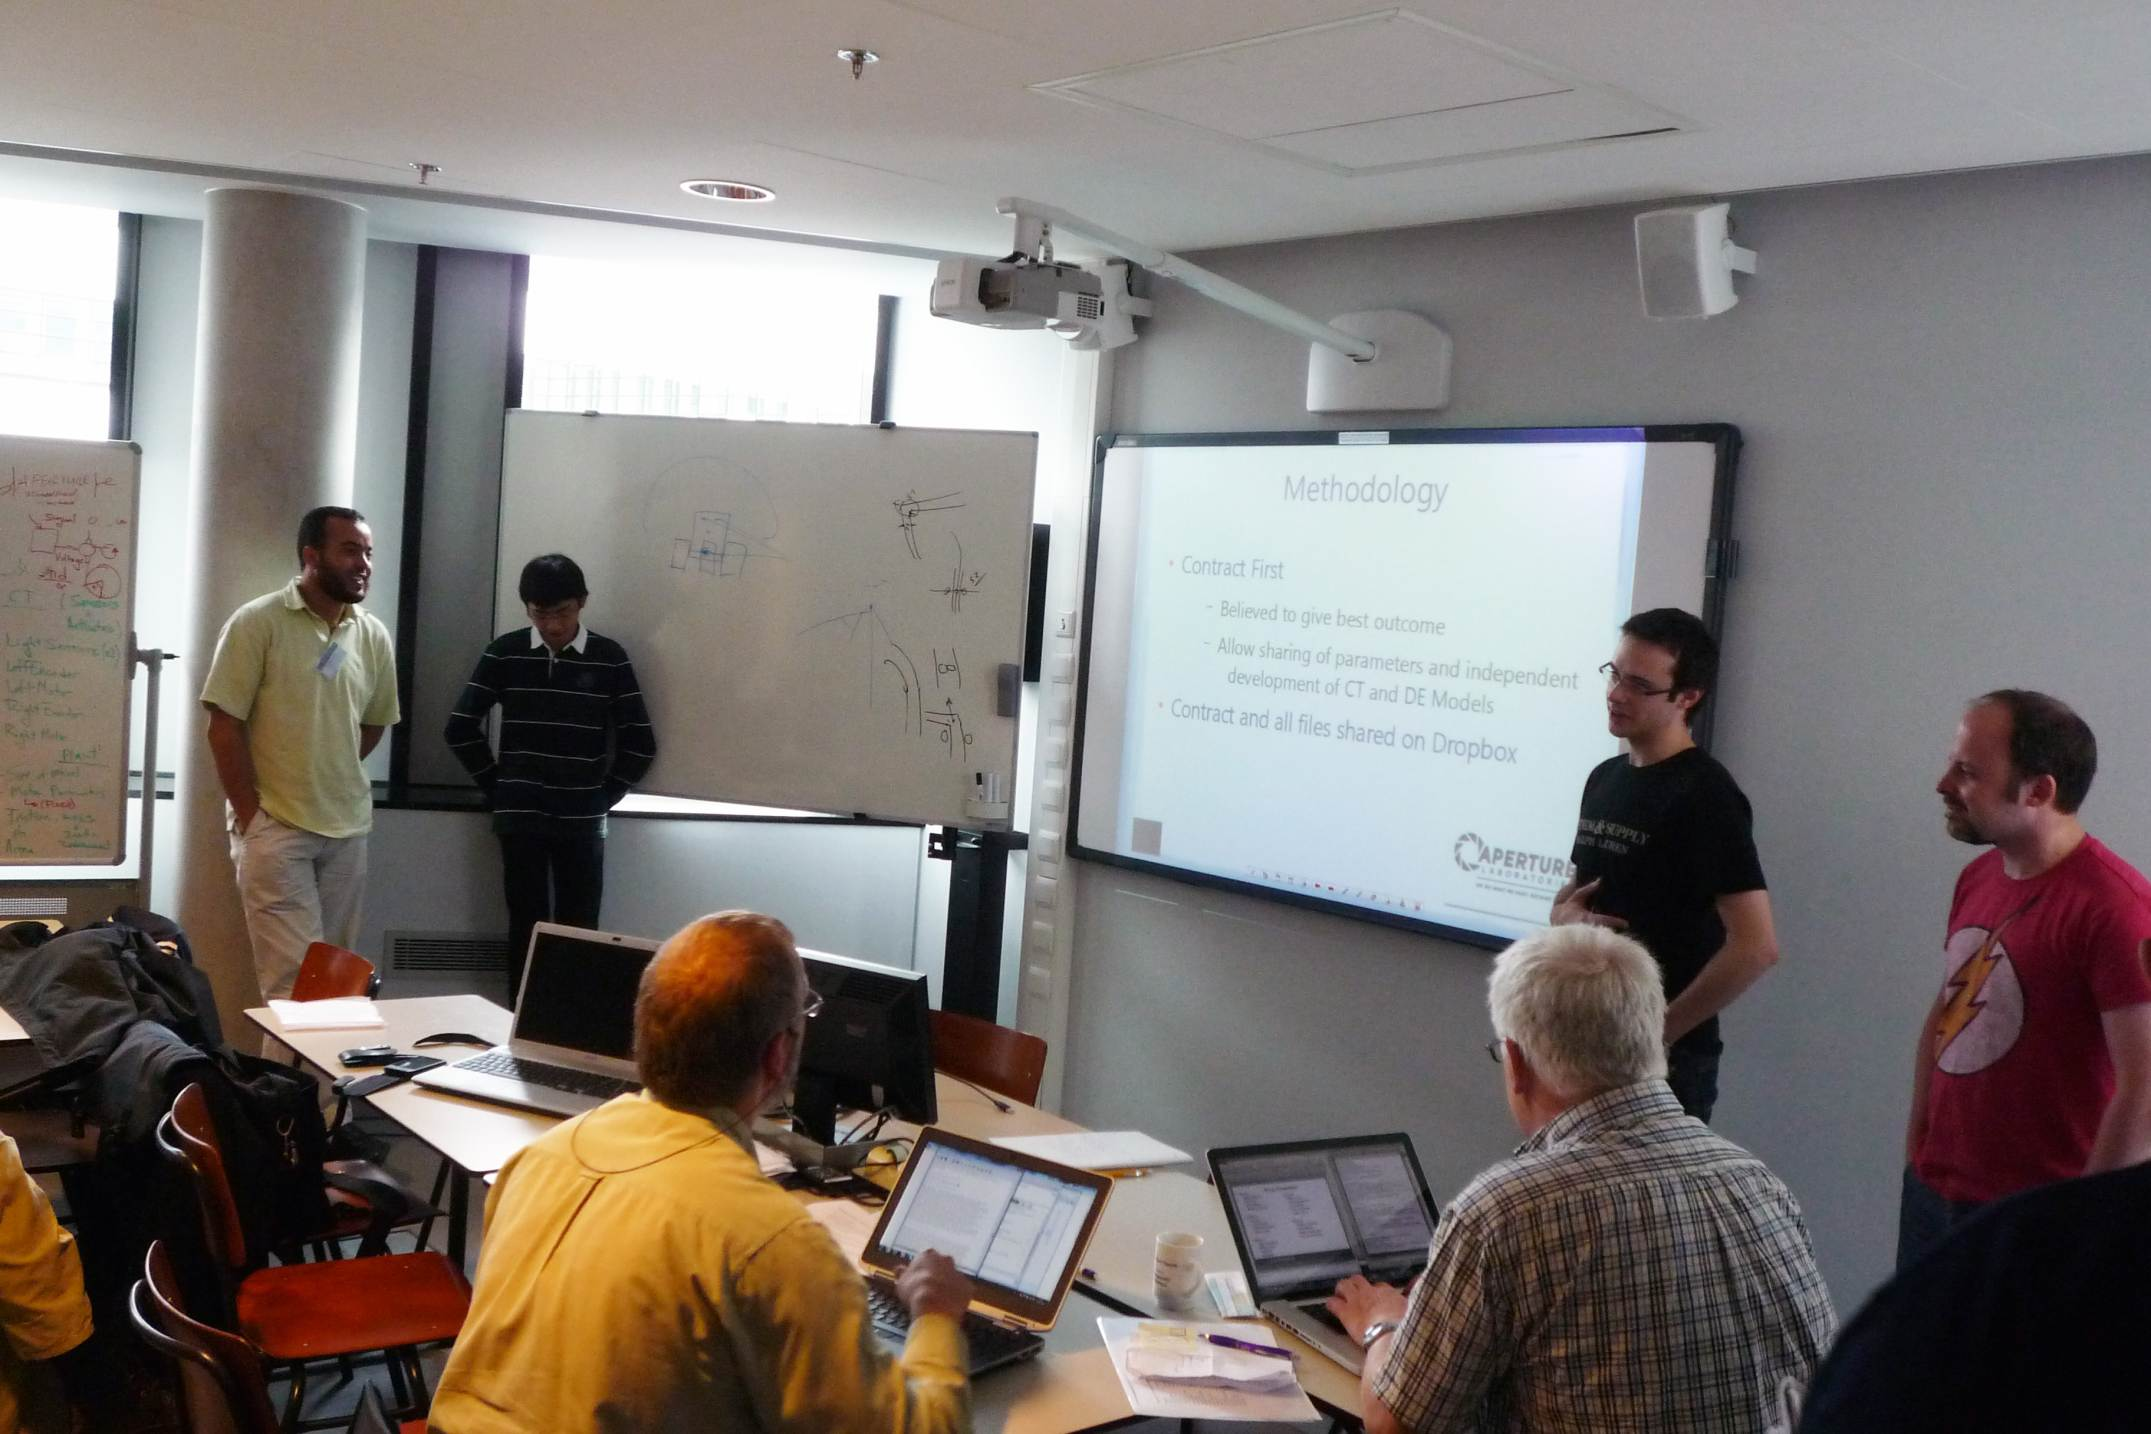
\includegraphics[width=\picsize]{summerSchoolModels/Group1} \quad
  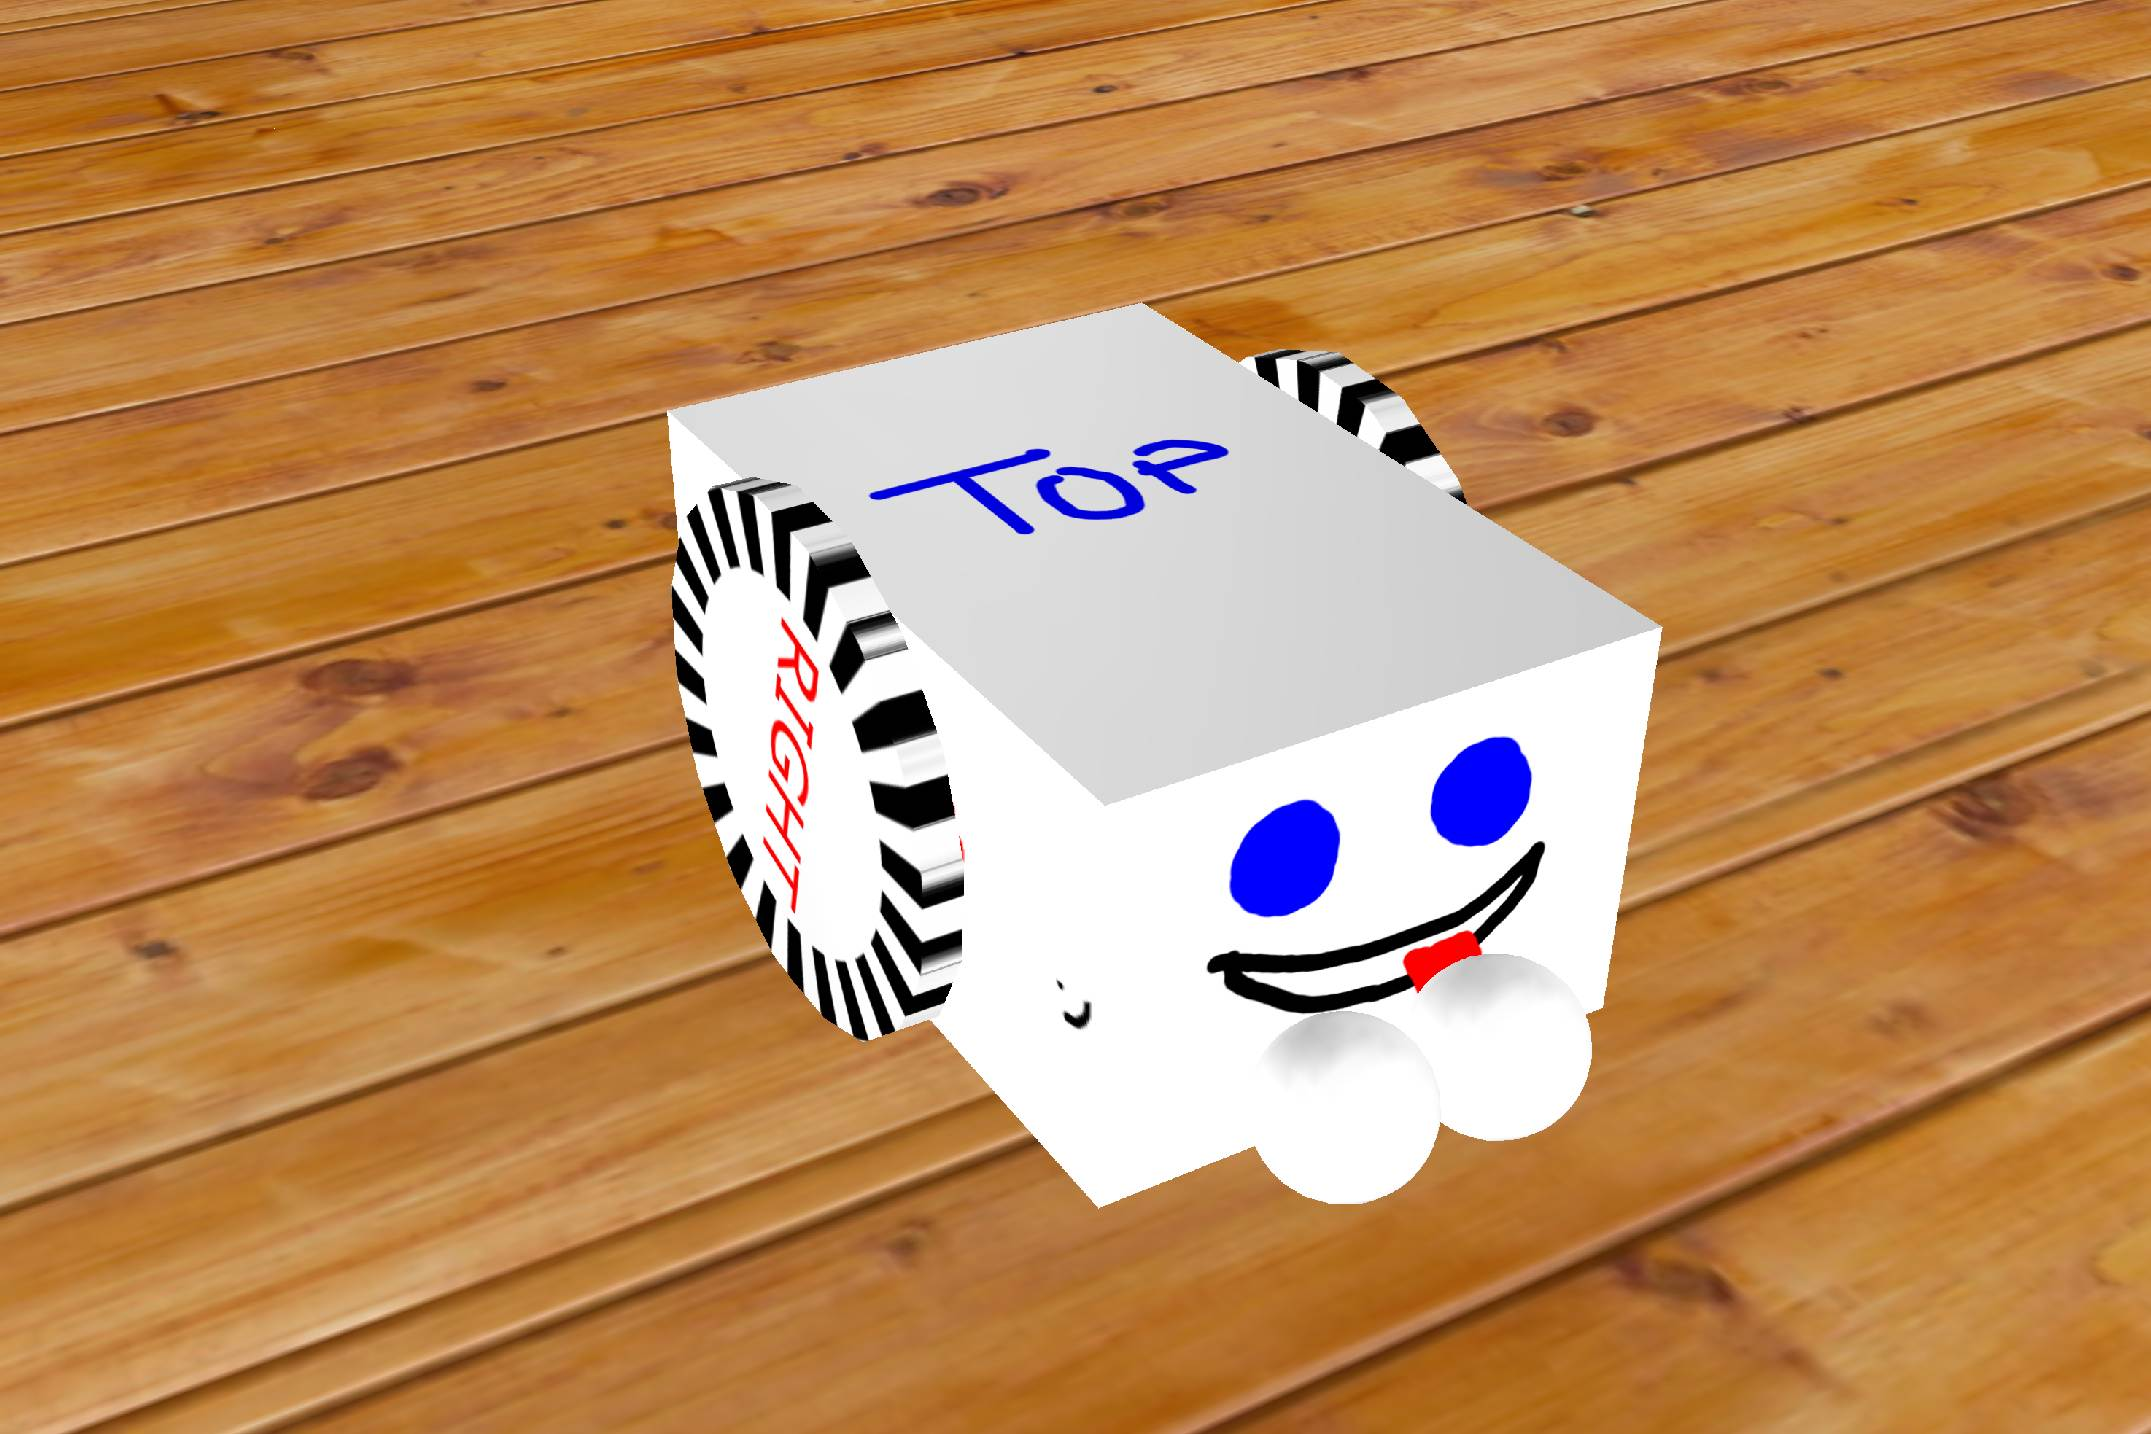
\includegraphics[width=\picsize]{summerSchoolModels/Group1robot}
} \\
\subfigure[Group 2]{\label{fig:group2}
  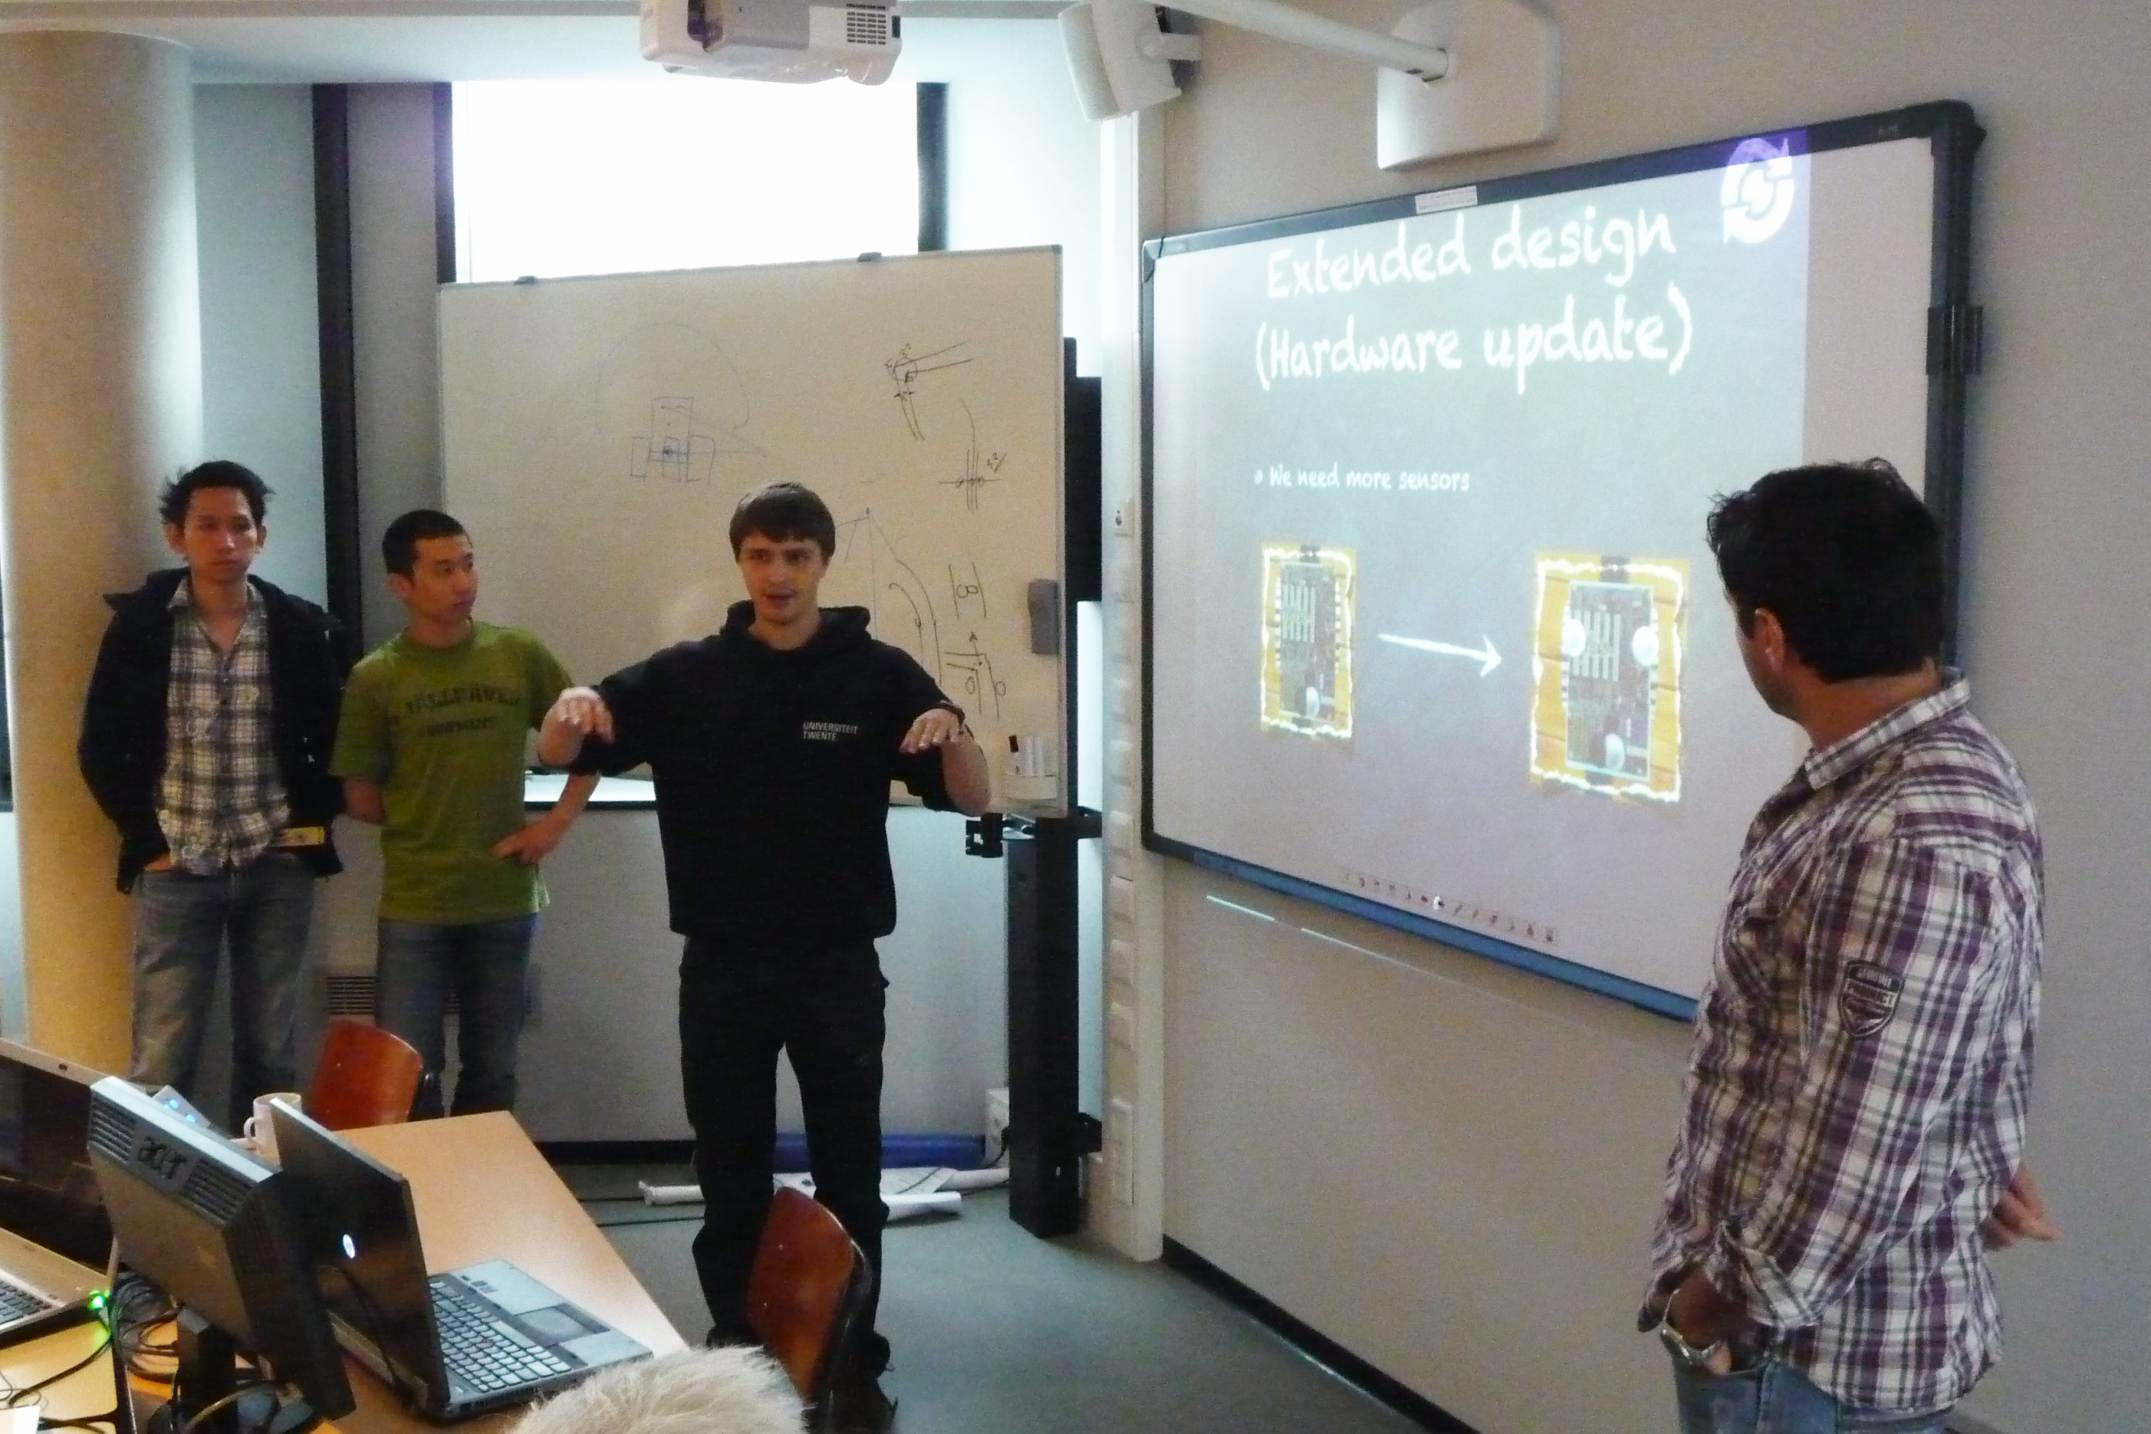
\includegraphics[width=\picsize]{summerSchoolModels/Group2} \quad
  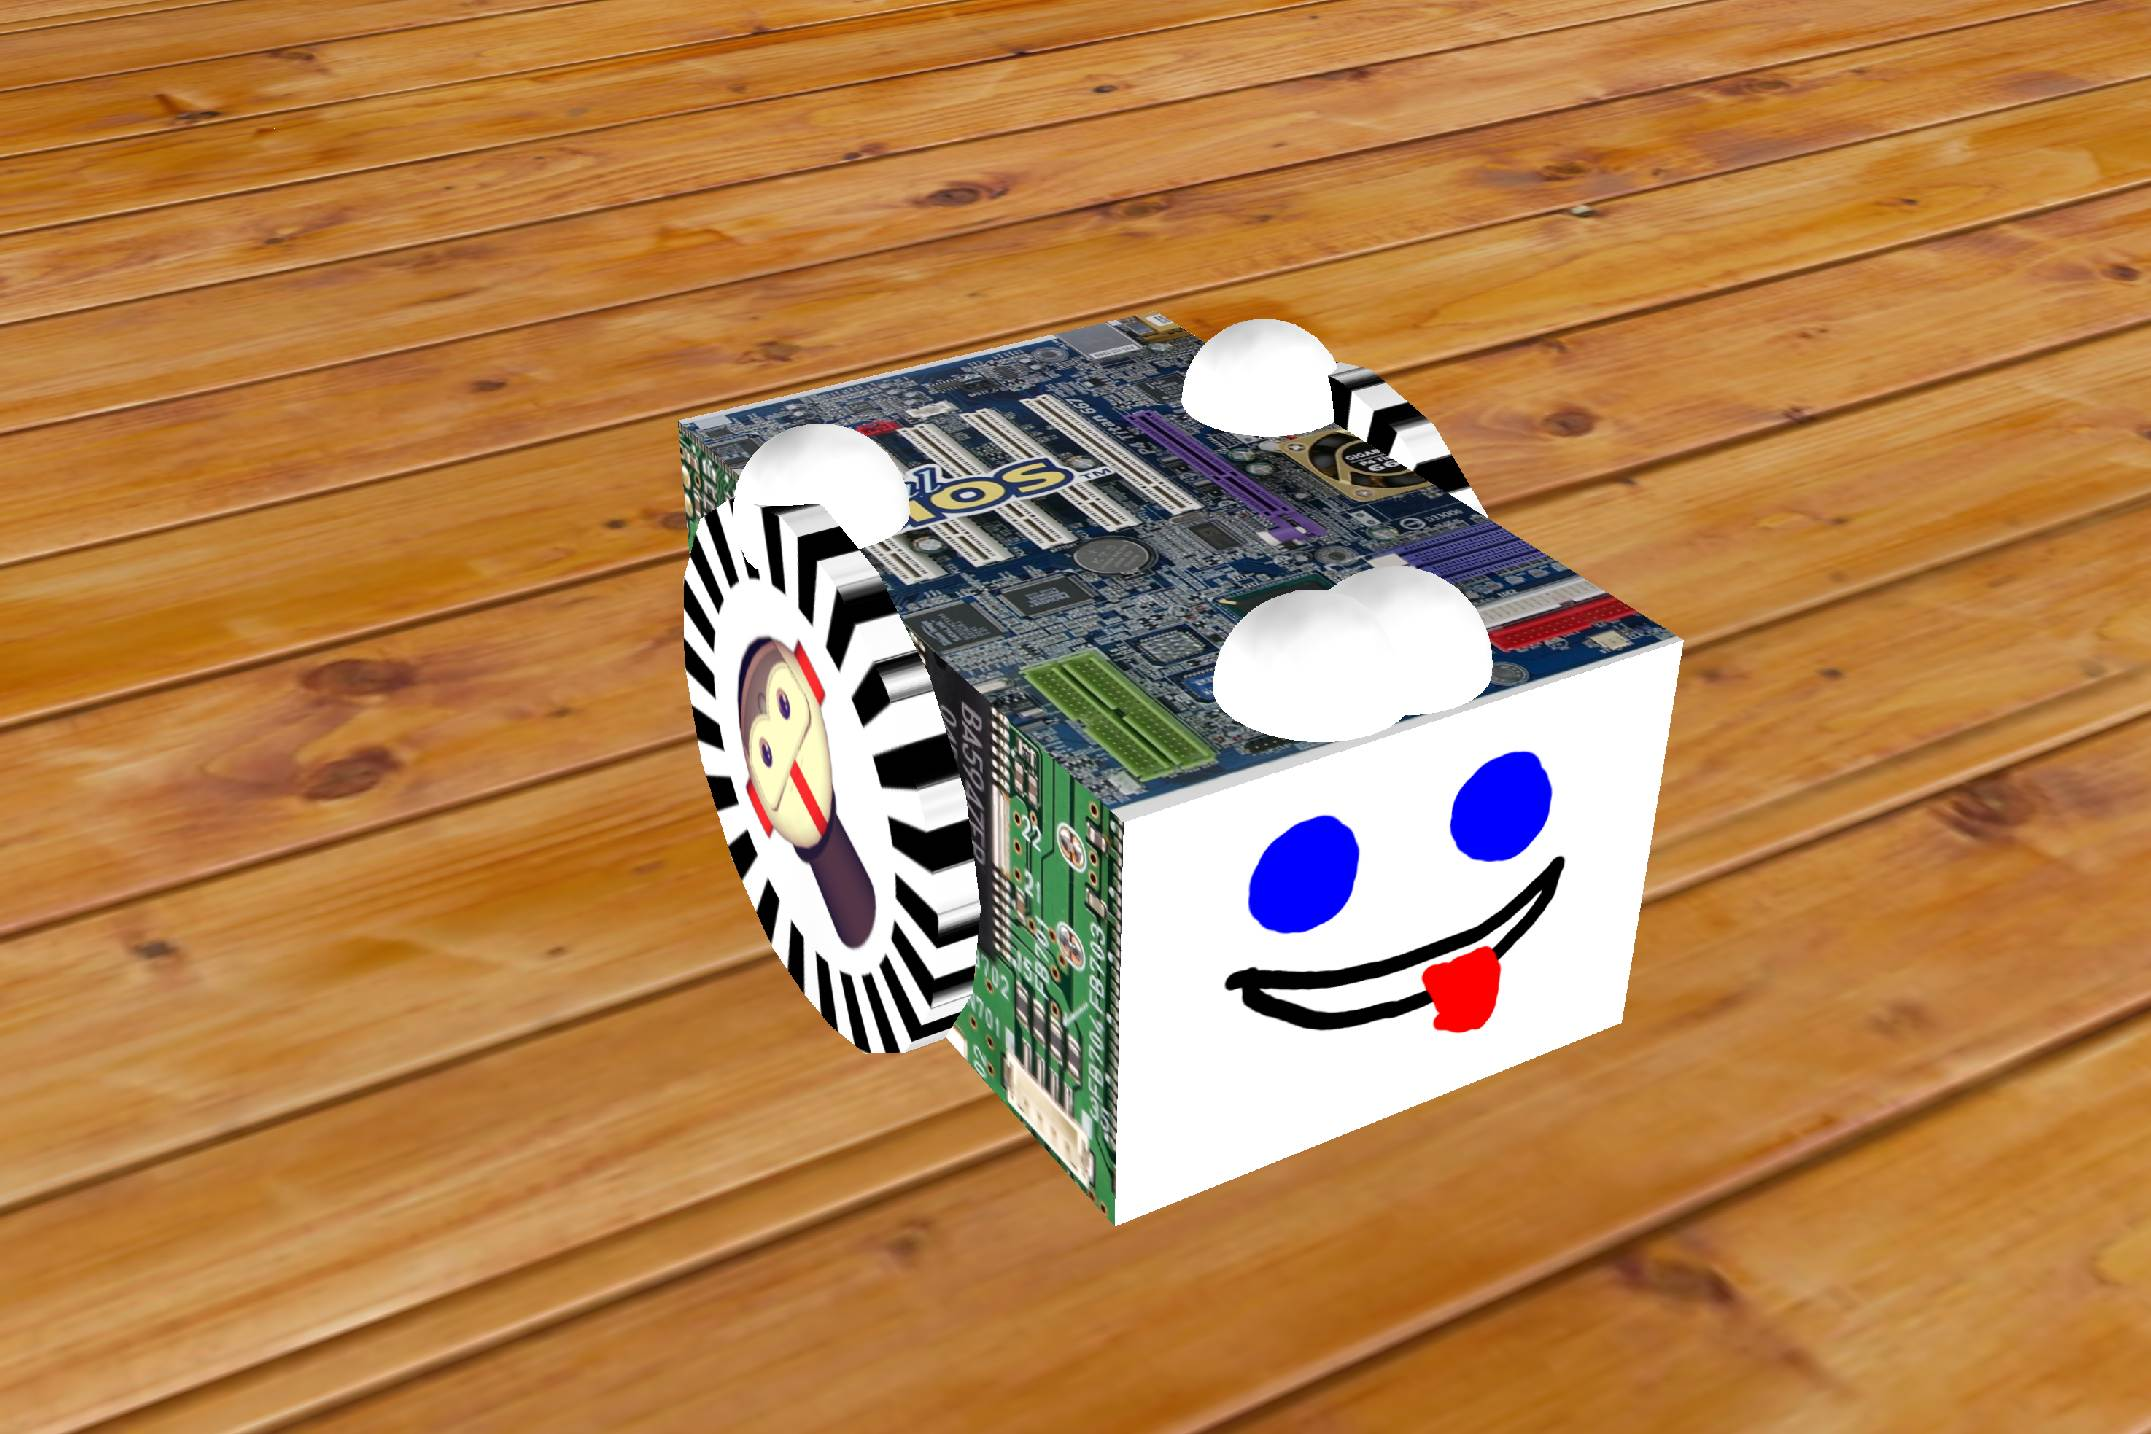
\includegraphics[width=\picsize]{summerSchoolModels/Group2robot}
} \\
\subfigure[Group 3]{\label{fig:group3}
  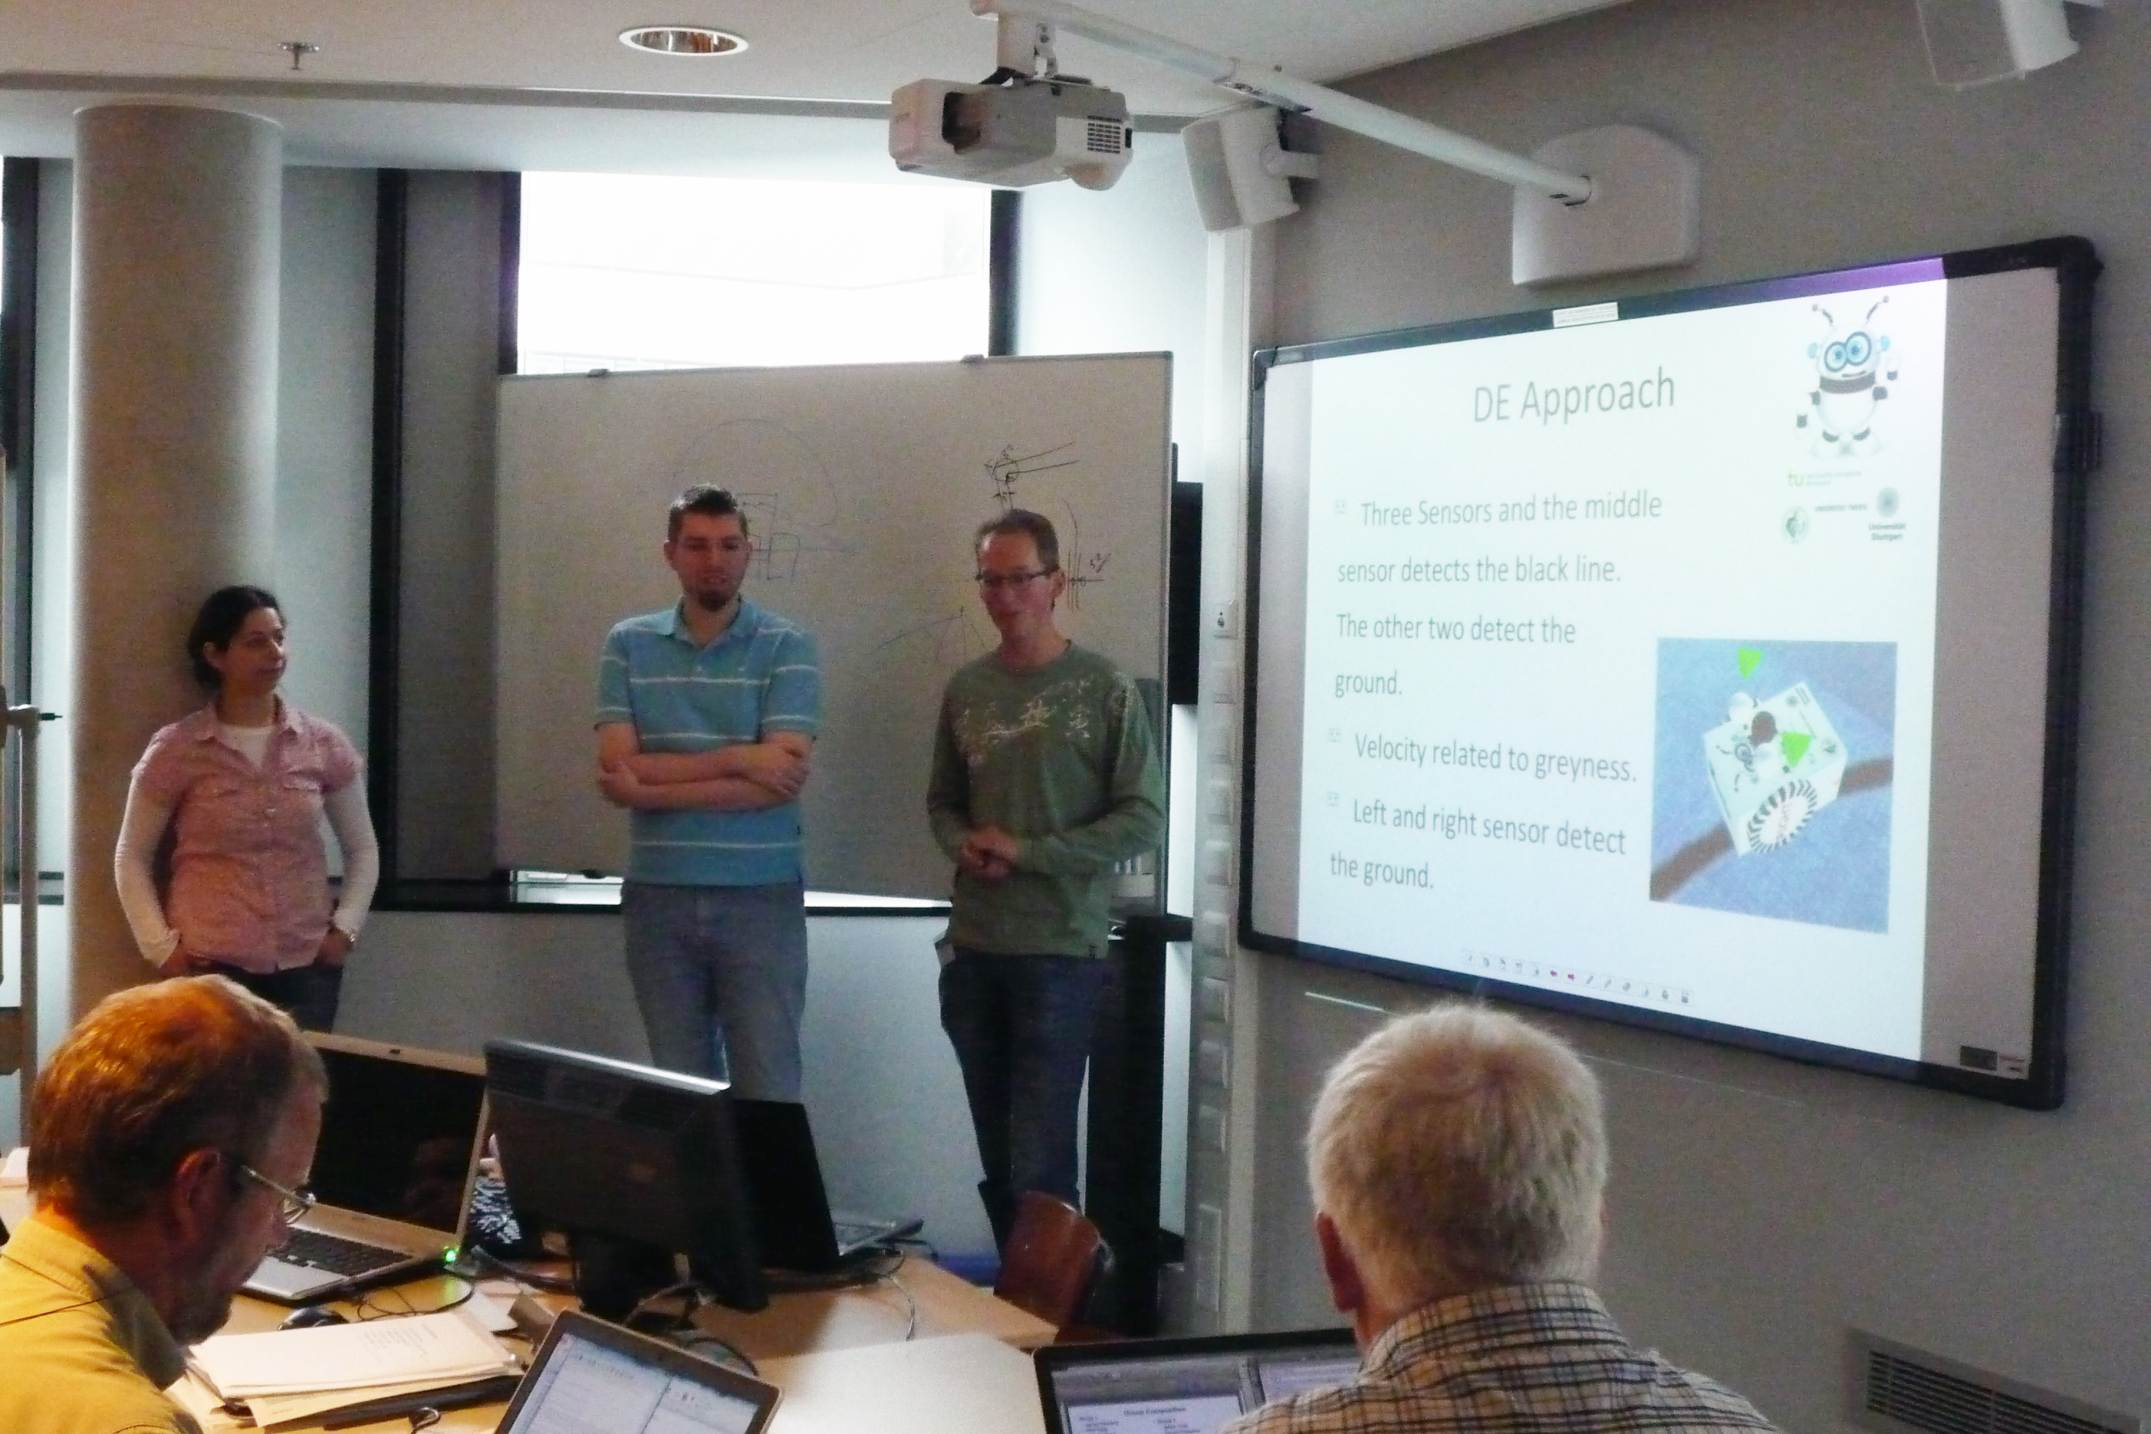
\includegraphics[width=\picsize]{summerSchoolModels/Group3} \quad
  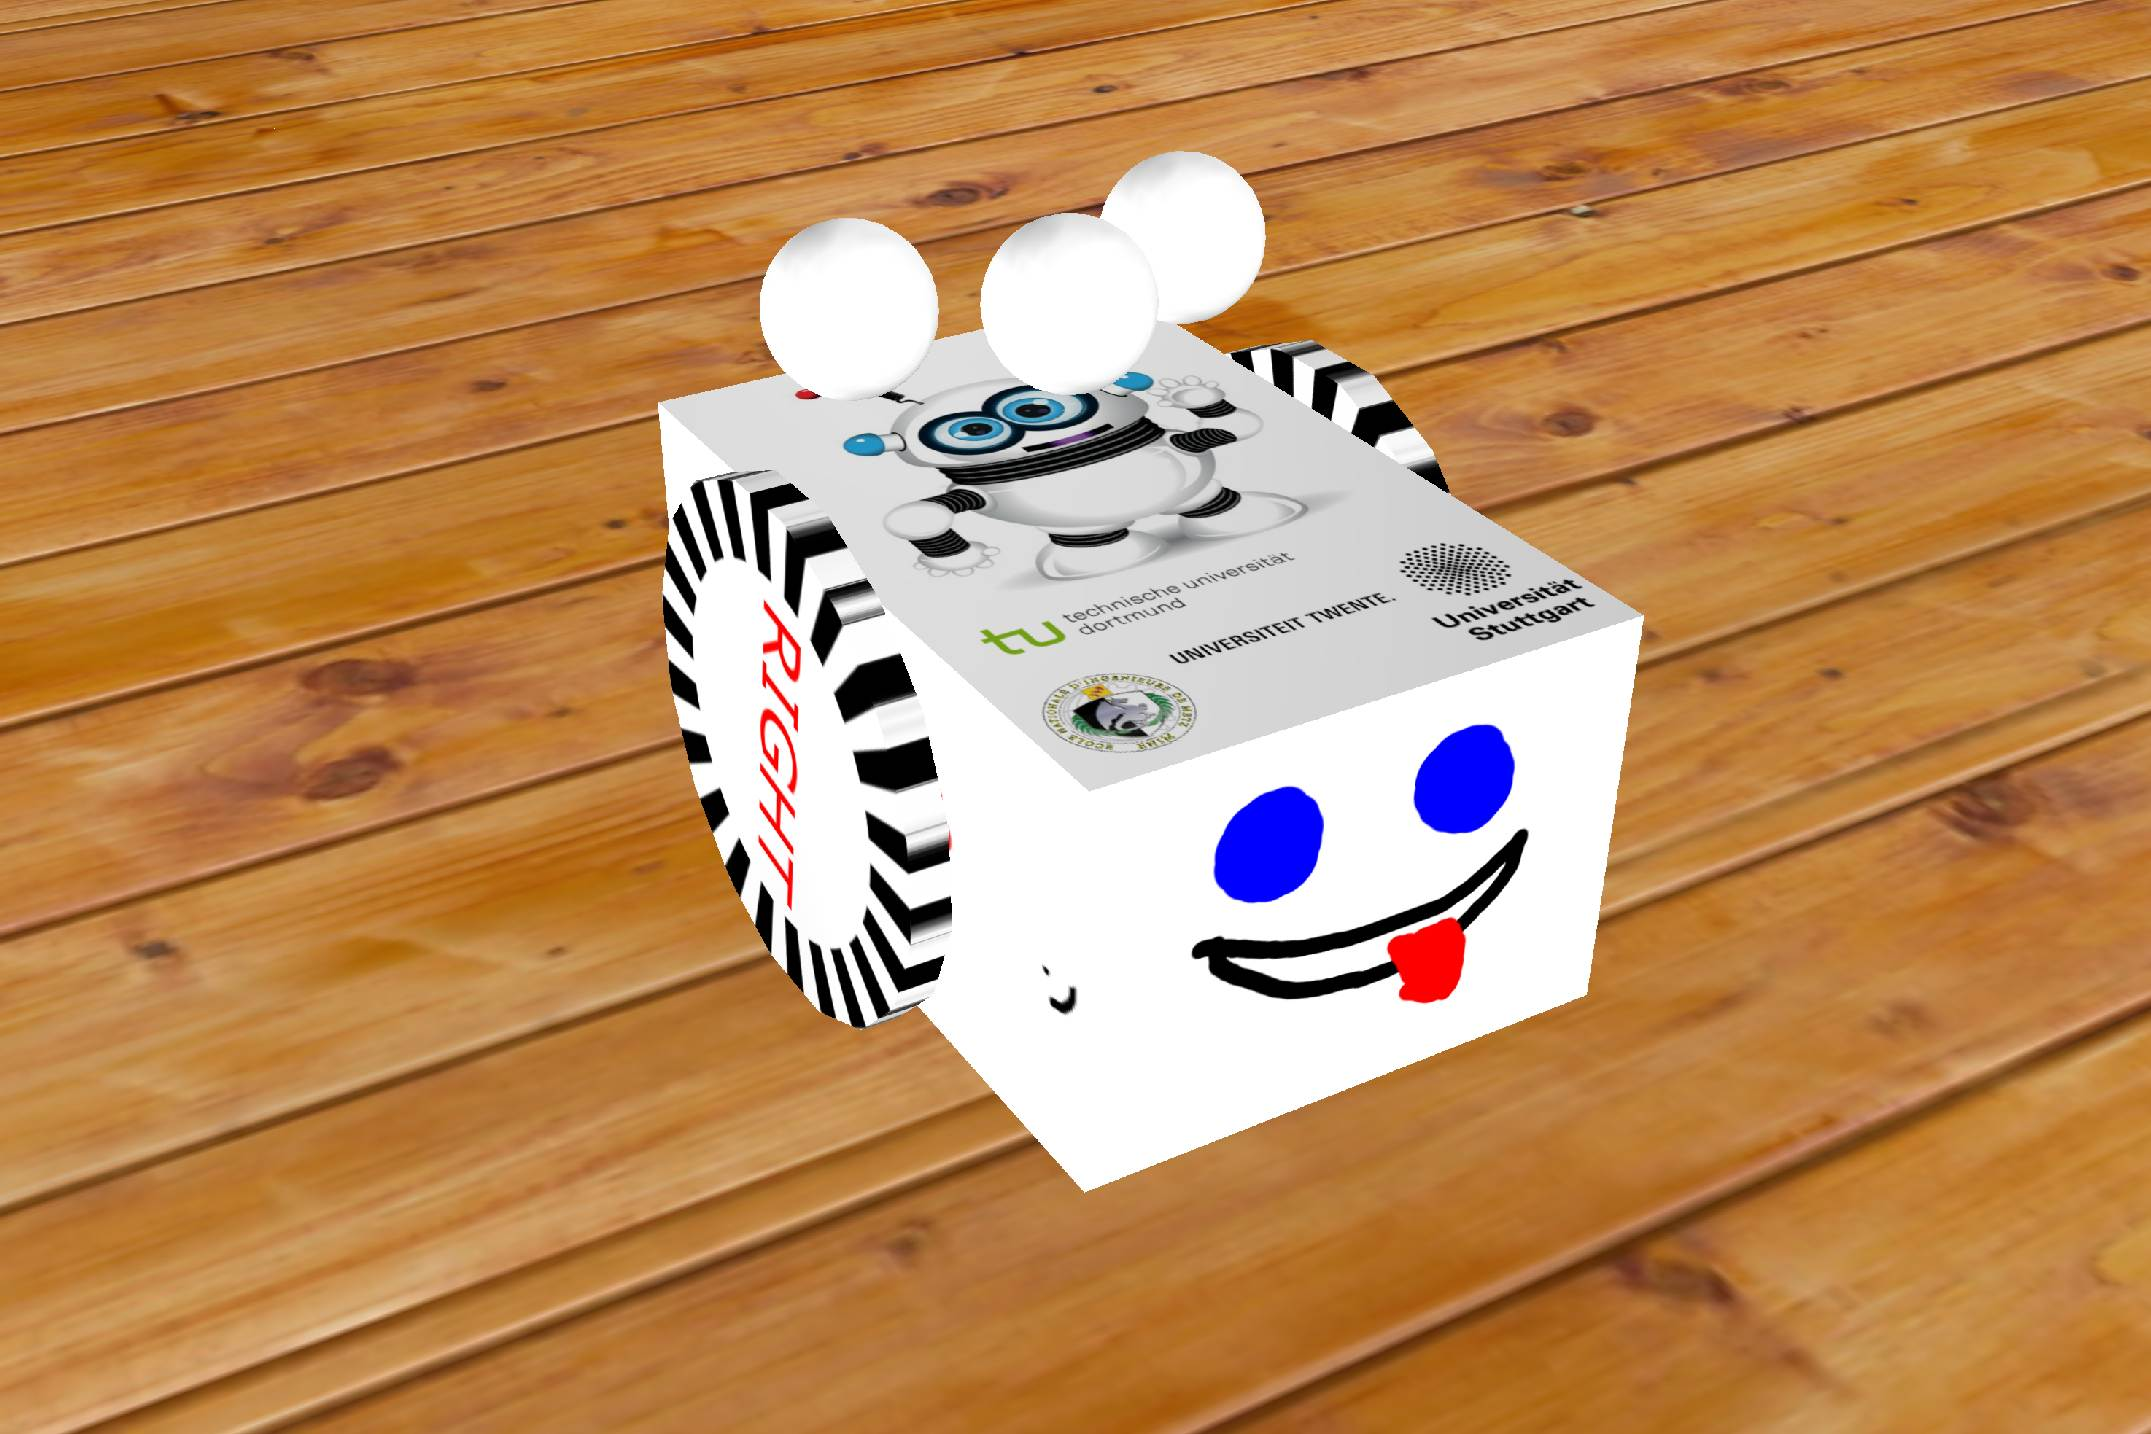
\includegraphics[width=\picsize]{summerSchoolModels/Group3robot}
} \\
\subfigure[Group 4]{\label{fig:group4}
  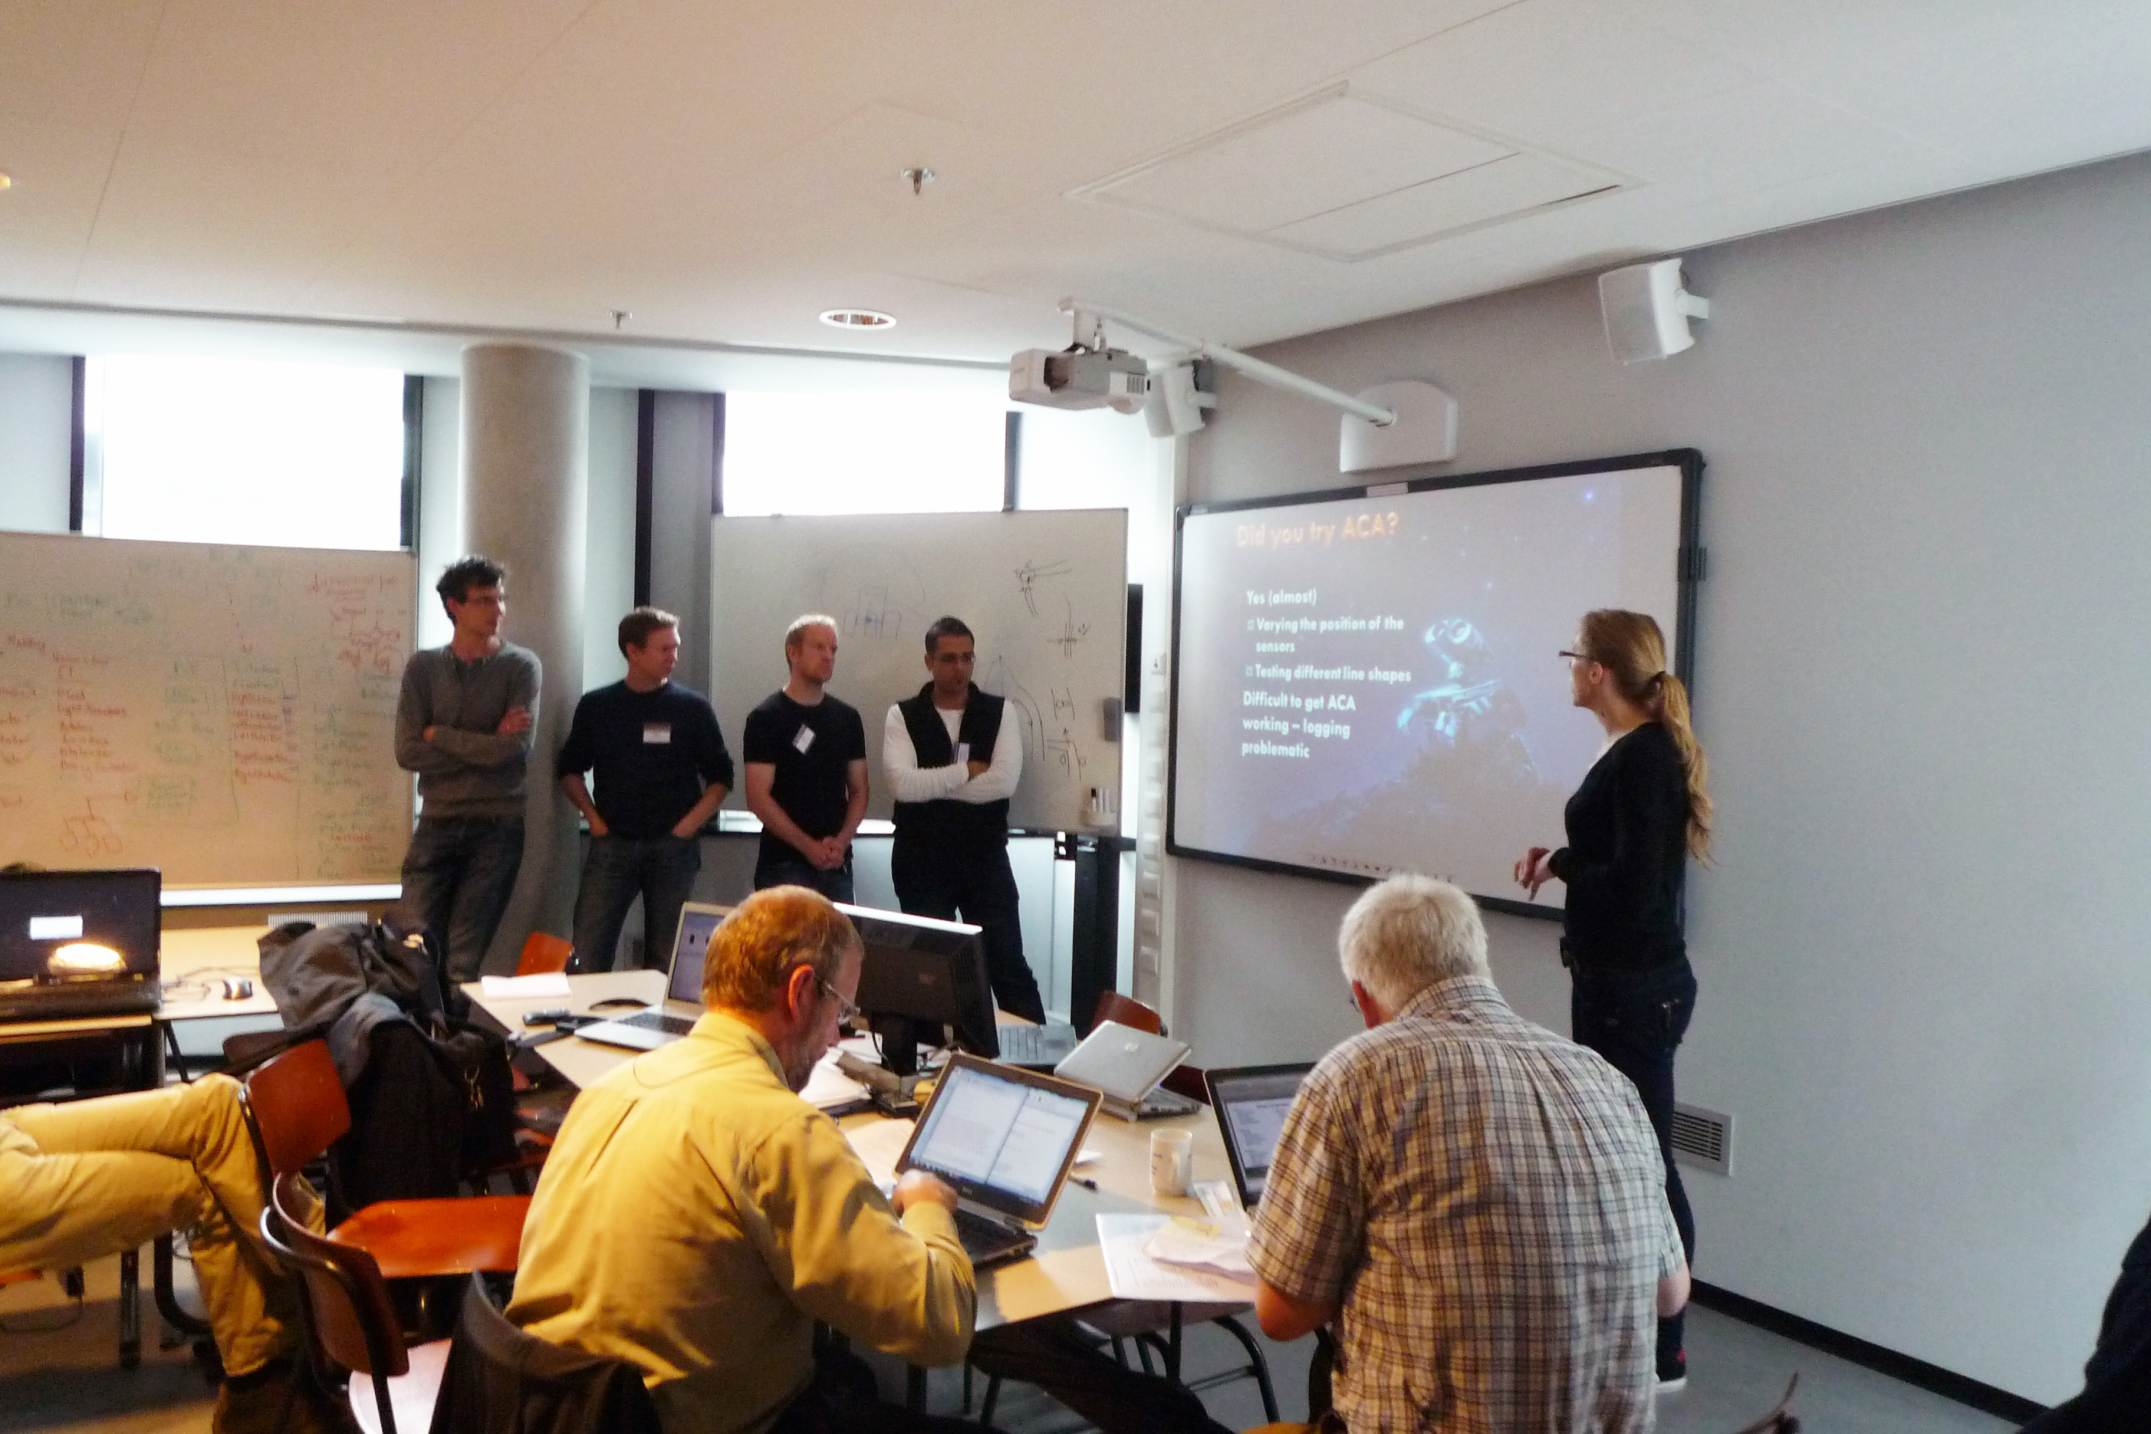
\includegraphics[width=\picsize]{summerSchoolModels/Group4} \quad
  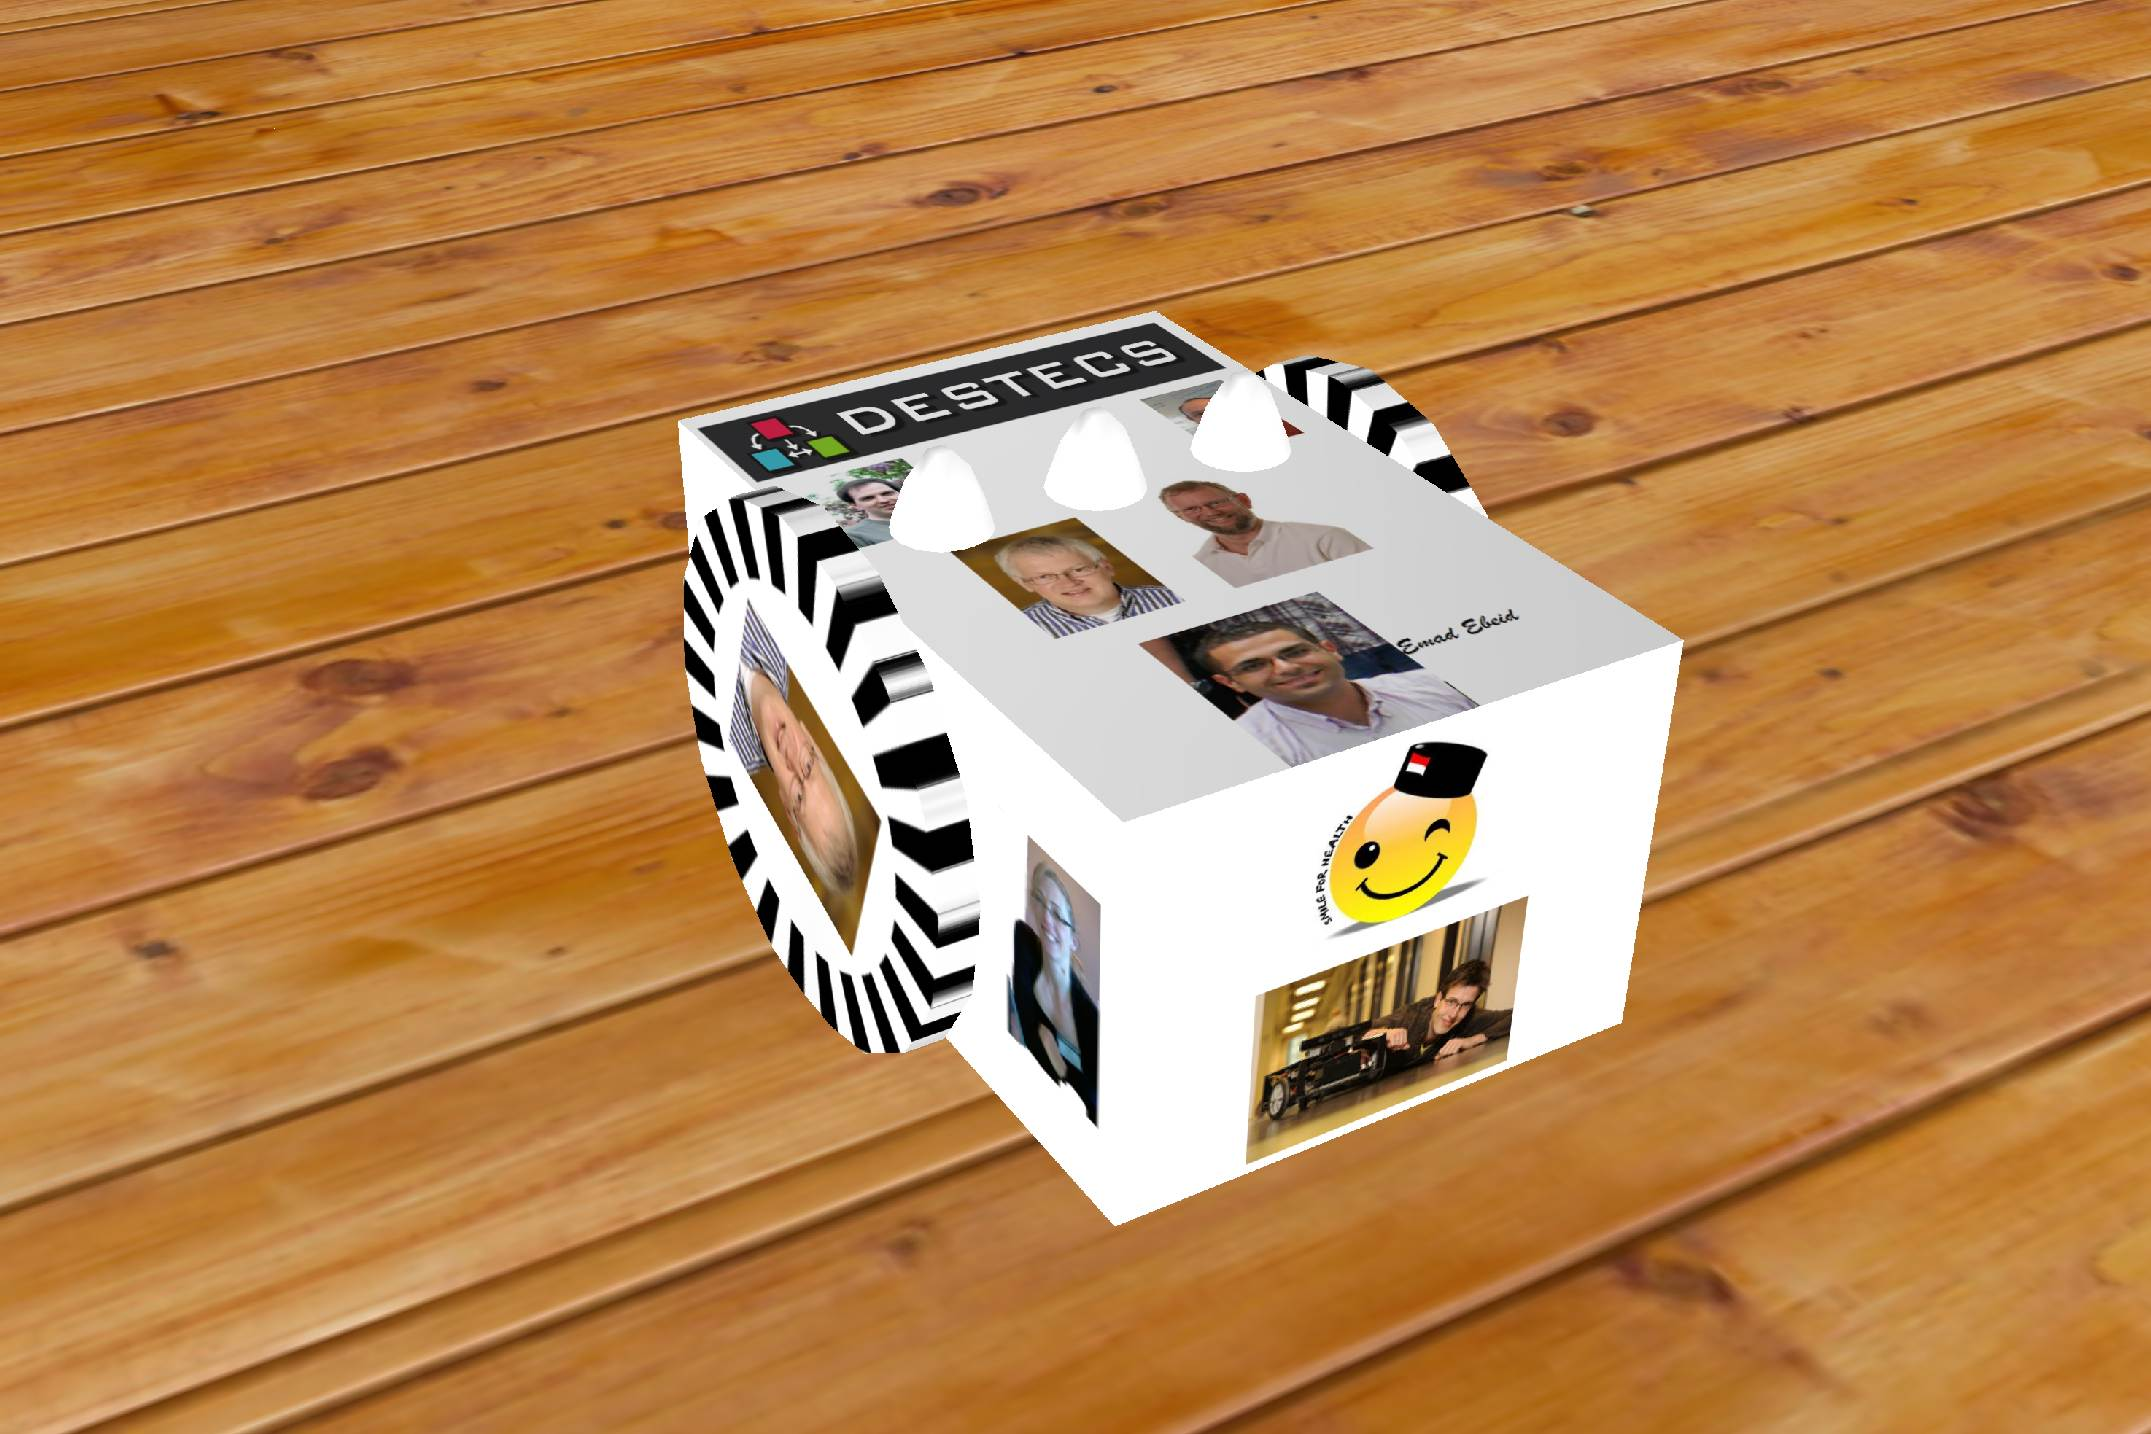
\includegraphics[width=\picsize]{summerSchoolModels/Group4robot}
} \\
\subfigure[Group 5]{\label{fig:group5}
  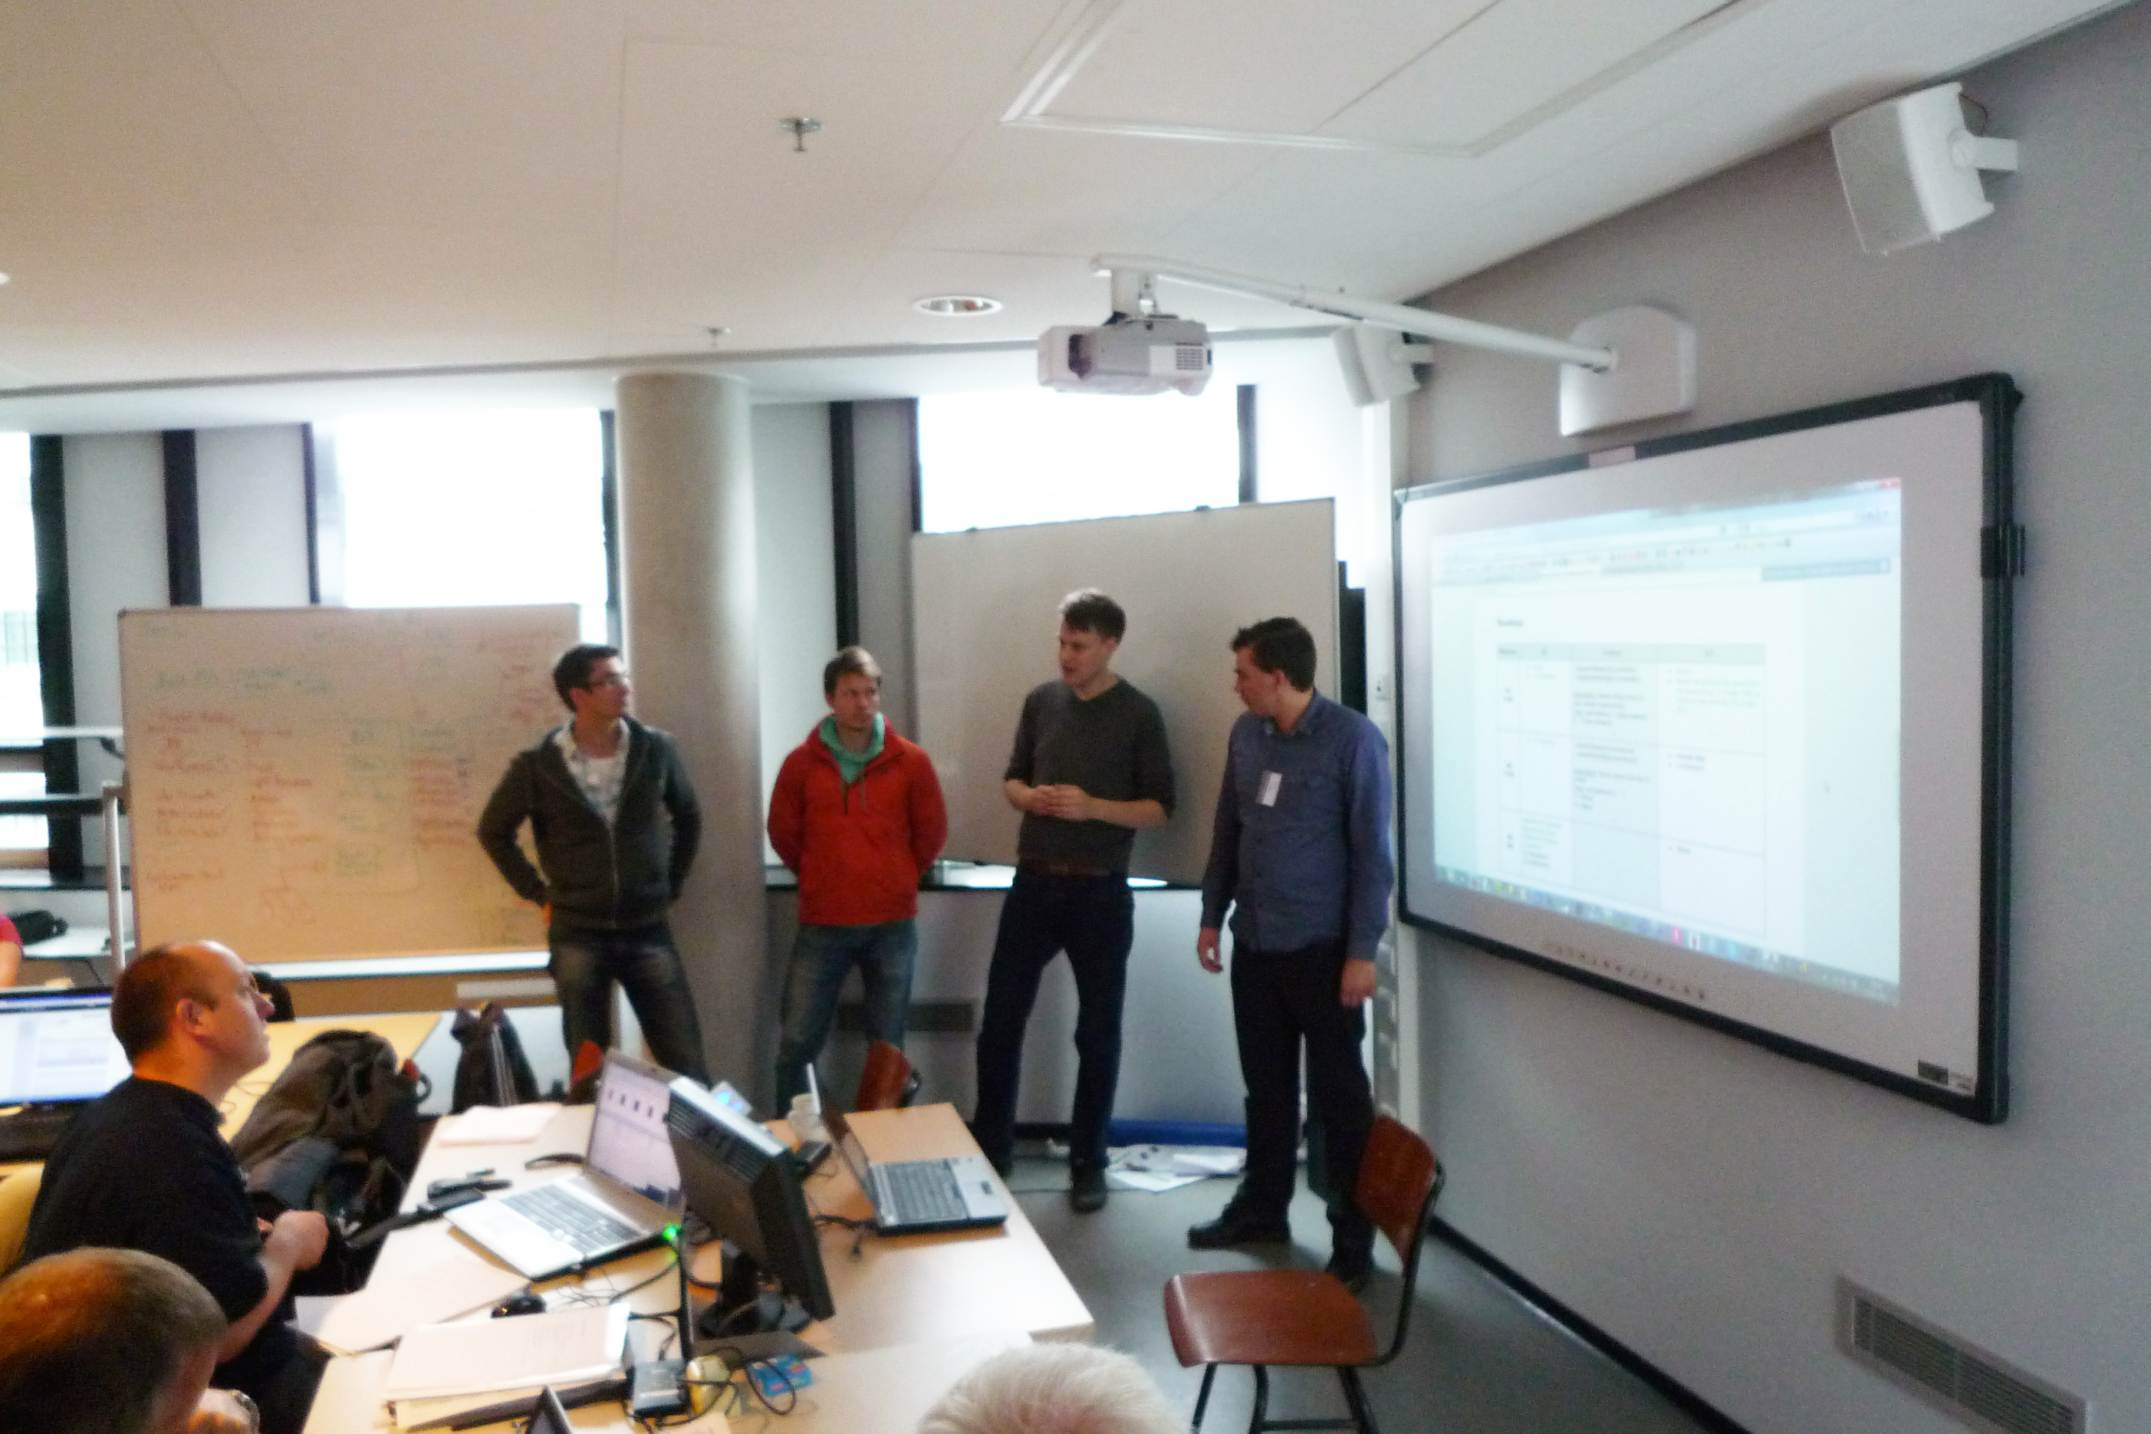
\includegraphics[width=\picsize]{summerSchoolModels/Group5} \quad
  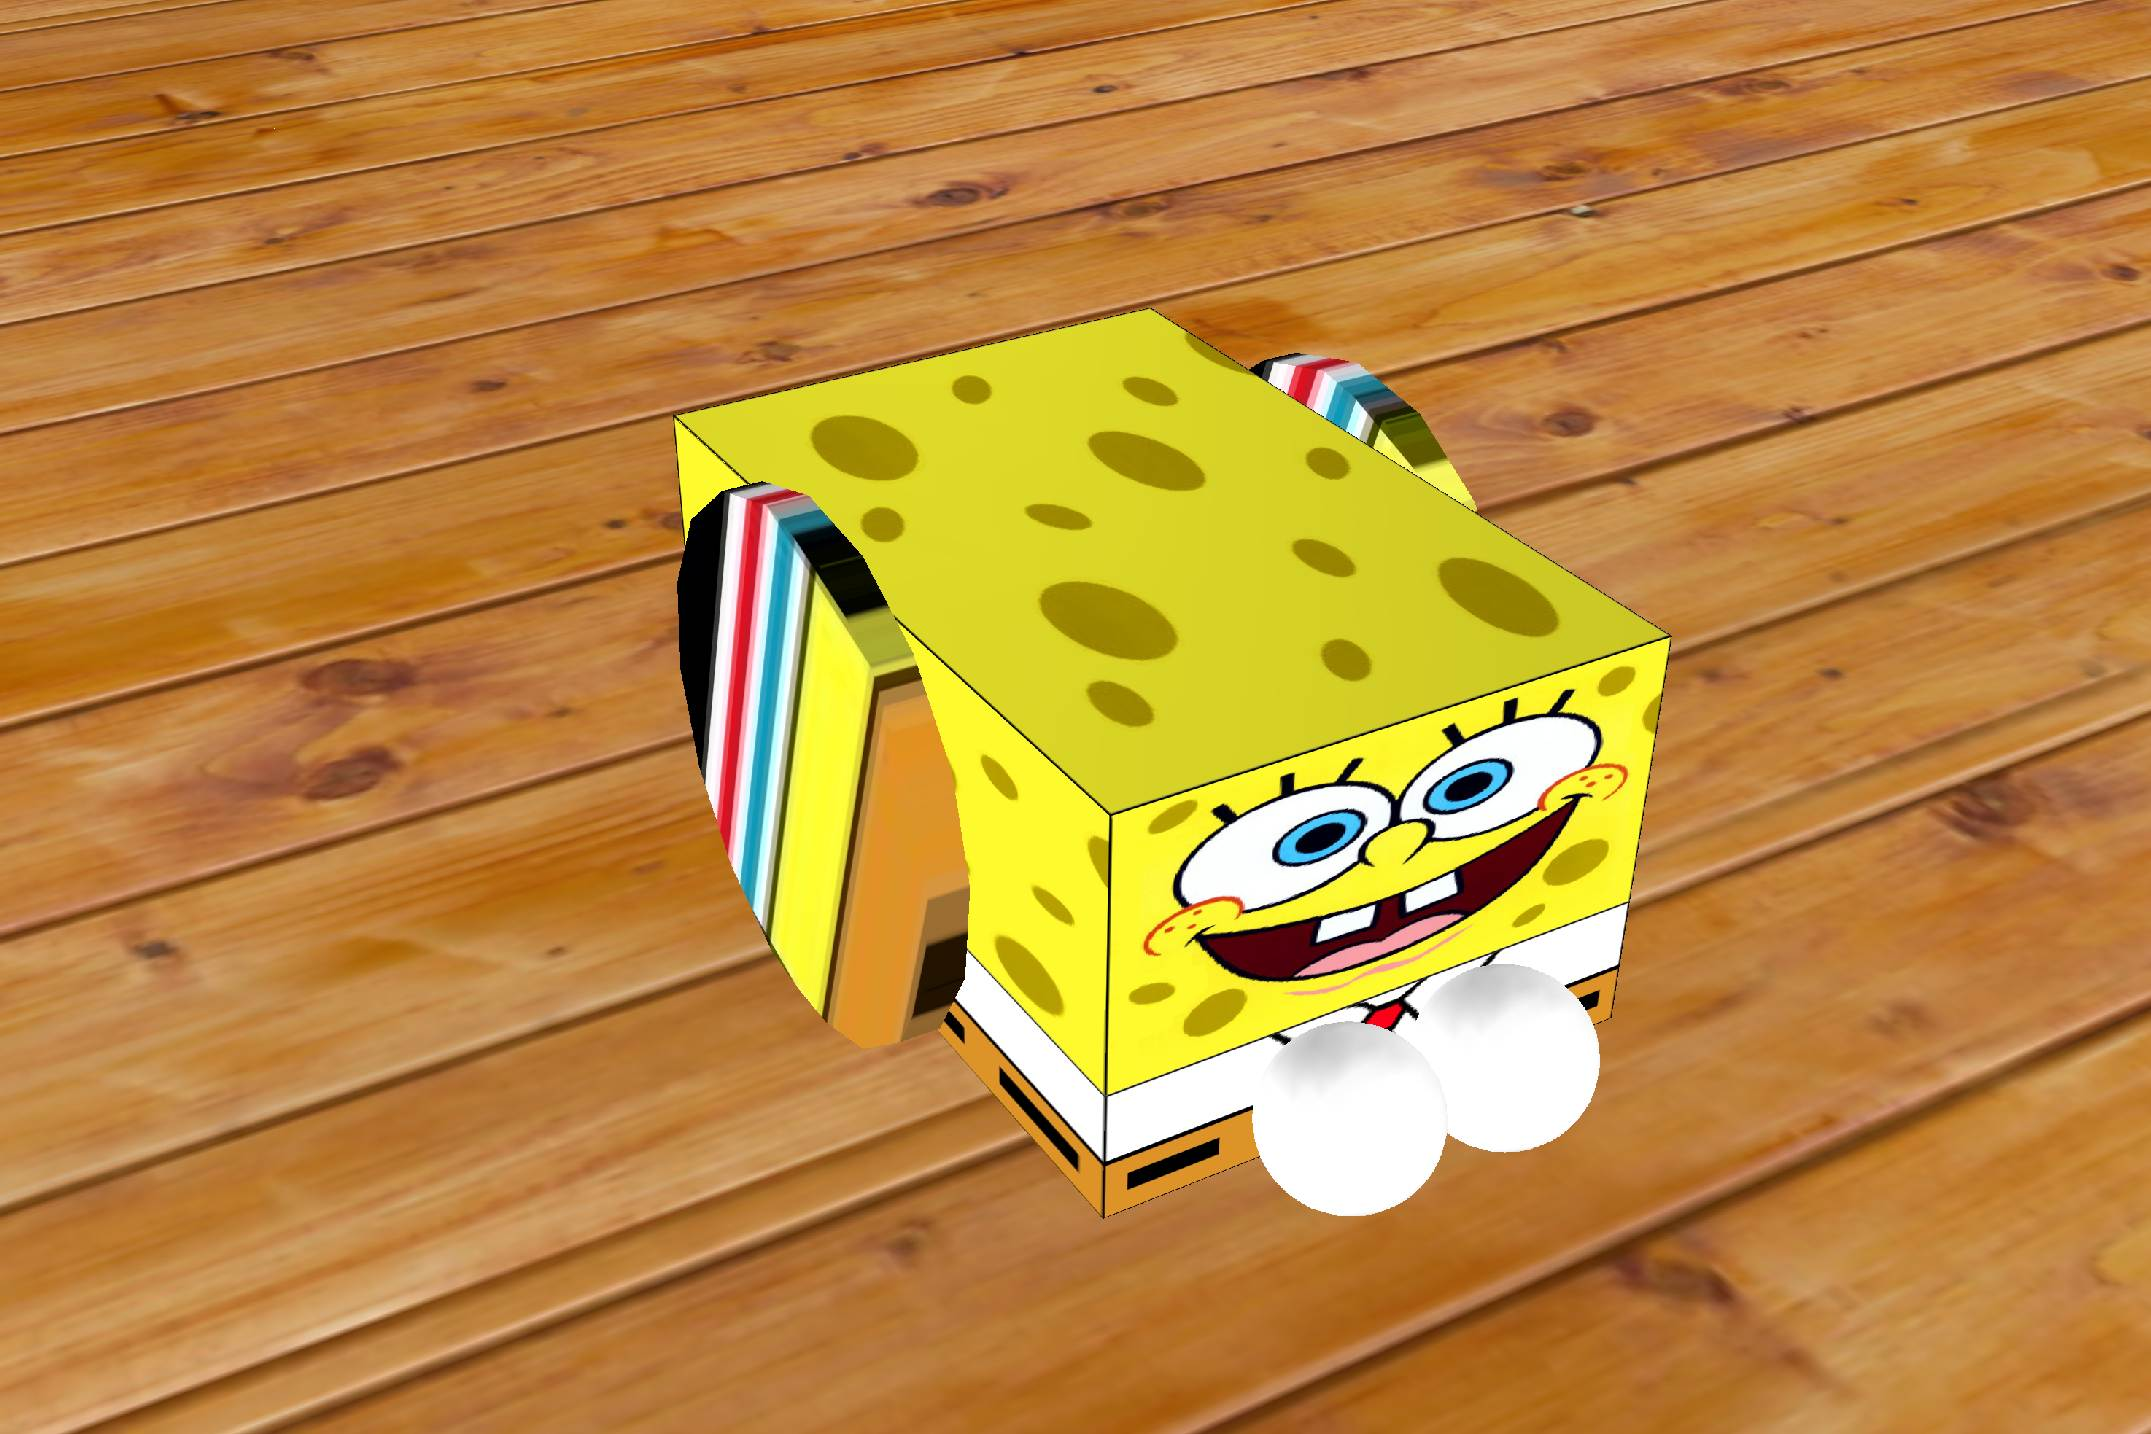
\includegraphics[width=\picsize]{summerSchoolModels/Group5robot}
}
\caption{Photograph of each group and a screenshot of their robot design}
\label{fig:groupphotos}
\end{figure}


\section{Group 1}

\subsection{Case Description}
Group 1 opted for a design with two sensors (left and right), placed
symmetrically.  The layout chosen is not completely finished and may
not handle all maps equally well - it may cope with some angles and
corners better than others.  Group 1's model is an example of a model
that prioritises speed when executing turns, as both wheels continue
to turn as fast as is practical whilst turning.  Some other models
made different decisions and either halted one wheel entirely or
reversed one wheel to execute a turn.

\subsection{Contract} The contract contains six variables of type
\keyw{real}. Two \emph{monitored} variables, \texttt{leftLSValye} and
\texttt{rightLSValue}, are used to represent inputs from the
line-detecting sensors on the left and the right respectively.  Two
further \emph{monitored} variables, \texttt{leftEncoderValue} and
\texttt{right\-Encoder\-Value}, are used to represent input from the
sensors used to count revolutions of the wheels.  This information is
necessary in order to calculate distance travelled, a requirement of
the exercise.

Two \emph{controlled} variables of type \keyw{real},
\texttt{leftMotorDC} and \texttt{rightMotorDC}, are used to produce
signals to the motor for the left and right wheels respectively.

The contract also includes the five shared design parameters described
for all groups in Section \ref{chap:summerschoolintro}.

\subsection{Discrete-event}
In the DE model, the \texttt{System} class instantiates two instances
of the \texttt{Sensor} class to represent sensors placed on the left
(\texttt{leftLineSensor}) and the right (\texttt{rightLineSensor}).
In addition \texttt{System} instantiates two instances of
\texttt{Actuator} (\texttt{leftPWM} and \texttt{rightPWM}) to provide
signals to the motors for the left and right wheels.

To provide a closed feedback loop, two more \texttt{Sensor} instances
are created to represent the encoders monitoring actual revolutions
turned by the wheels on the left (\texttt{leftEncoder}) and on the
right (\texttt{rightEncoder}).

Finally, \texttt{System} creates an instance of
\texttt{ModalController} to provide controller functionality, and
deploys it onto a single CPU.  \texttt{ModalController} provides the
primary logic for the robot.  A number of modes are defined; an
initial mode sees the robot start moving forward, hunting for the
initial pattern.  Next is a calibration phase where the robot
continues as it follows the initial pattern, and a line-following
phase where the actual line begins.  A final phase sets the robot at
rest after the end of the line is identified.  The robot reduces the
speed of the left wheel to turn left if the left sensor detects the
line on the ground, and it reduces the speed of the right wheel to
turn right if the right sensor detects the line.

\subsection{Continuous-time}
As with all the other groups, the CT model includes blocks to provide
an implementation of robot physics (\texttt{RobotPhysics}) and data
for the 3D simulation (\texttt{DataFor3D}).

A \texttt{controller} class handles interaction with the DE model.
The CT model includes two blocks to represent the encoders for the
wheels on the left (\texttt{encoderLeft}) and on the right
(\texttt{encoderLeftRight}). Each encoder accepts input (data representing
the number of black or white areas on the wheel which have moved past
the sensor), and incorporates blocks that convert this data into a
count of the number of revolutions the wheel has made.

Input from the \texttt{controller} is passed to \texttt{RobotPhysics}
for some processing and is then made available to the encoders.
Output from \texttt{RobotPhysics} is also passed to a block
\texttt{pos\-Con\-ver\-ter} which is responsible for calculating current
position.  This block interacts with blocks \texttt{floorMapLeft} and
\texttt{FloorMapRight}, which act as lookup tables for interpreting what is
currently visible in the map.



%\subsection{Scenarios}



\section{Group 2}
\subsection{Case Description}
Group 2 employ four line-following sensors for their robot - two (for
the left and for the right) placed forward and two (also for left and
right) placed further back.  The sensors mounted towards the back of
the robot are used to identify sharp turns, when the course of the
line may be so sharp that it turns back behind the robot's current
position.  Front-mounted sensors may find such a scenario difficult to
detect, assuming that if the line cannot be seen ahead or on one side
then it must have reached the finish point.

Group 2 also made the decision to vary the speed of the robot, so that
on tighter corners or on more straightforward elements of the track,
the robot can move more quickly.  This is possible because the
presence of two extra sensors towards the back of the robot in
addition to two on the front allows corners and curves to be
categorised as shallow (visible to the front sensors) or steep
(visible to the back sensors and not to the front ones).  Different
turning speeds can then be selected for these two types of corner.

\subsection{Contract}
The contract contains six variables of type \keyw{real}. Four
\emph{monitored} variables, \texttt{lineSensorLeft},
\texttt{lineSensorRight}, \texttt{lineSensorLeftB} and
\texttt{lineSensorRightB}, are used to represent inputs from the four
line-detecting sensors (front left and front right, back left and back
right respectively).  Two further \emph{monitored} variables,
\texttt{wheelPosLeft} and \texttt{wheelPosRight}, are used to
represent input from the sensors used to count revolutions of the left
and right wheel.  This information is necessary in order to calculate
distance travelled, a requirement of the exercise.

Two \emph{controlled} variables of type \keyw{real},
\texttt{motorVoltageLeft} and \texttt{motorVoltageRight}, are used to
produce signals to the motor for the left and right wheels
respectively.

Group 2 did not make use of any shared design parameters.

\subsection{Discrete-event}
The \texttt{System} class in Group 2's model begins by creating six
instances of the class \texttt{Abstract\-Sen\-sor\-Real} for the six
sensors (four for line-detecting and two to act as encoders for the
wheels) and two instances of \texttt{AbstractActuatorReal} for the two
actuators.  The \texttt{Controller} class acts as a controller and has
the main thread of control; the \texttt{System} class deploys the
\texttt{Controller} to a single CPU.

At run time, \texttt{ActuatorReal} provides an implementation of
\texttt{AbstractActuatorReal}.  This class simply passes a signal to
the motors.  Implementations of the sensors are provided by different
classes for the sensors used as encoders, and the sensors uses as
line-detectors.  For the encoders, the class \texttt{EncoderSensor} is
used.  This class includes some short logic to convert the input from
the sensor representing the wheel encoder into a value for rotations
of the wheel.  For the line-detecting sensors, implementation is
provided by the class \texttt{SensorReal}, which simply handles data
produced by the sensor.

Like many other groups, Group 2 created different classes to contain
the functionality required for the different modes of operation.  The
\texttt{Controller} class stores a variable internally
(\texttt{ControllerMode}) which is of type
\texttt{AbstractControllerMode}.  At runtime different concrete
implementations of this abstract class are used during different modes
of operation.  The first implementation is provided by the
\texttt{InitilaizeControlMode} class, which proceeds until it can be
confirmed that the initial pattern on the ground has been detected and
that the robot has proceeded beyond it.  During the next mode the
concrete implementation of the \texttt{AbstractControllerMode} is
provided by \texttt{LineFollowingControlMode}.  This class proceeds on
a step-by-step basis.  For each step, the class first gathers readings
from each of the four line-detecting sensors.  In cases where both
front sensors can see the line, then the robot continues ahead at top
speed.  If the right front sensor can detect a line but the left
sensor cannot, then the robot should turn right.  Similarly, if the
left front sensor can detect a line but the right sensor cannot, then
the robot turns left.  \texttt{LineFollowingControlMode} checks for
situations where one of the rear-mounted sensors can detect a line
that is not visible to the front-mounted sensors.  In this case, it
assumes that there is a sharp corner in the line's course, and
executes a sharp turn in that direction.  If all four sensors detect
no line, then the robot is deemed to have finished the course.

Attempts are made to try and keep the speed as high as possible whilst
executing a turn; Group 2's robot keeps one wheel at \texttt{topSpeed}
and drops the speed of the other.  The model also differentiates
between sharp corners and shallow turns, and uses different speed
settings on the wheels to ensure that the robot turns more quickly in
a shorter distance on a sharper corner.

\subsection{Continuous-time}
As with all the other groups, the CT model includes blocks to provide
an implementation of robot physics (\texttt{RobotPhysics}) and data
for the 3D simulation (\texttt{DataFor3D}) .

Group 2's CT model employs a \texttt{Controller} block to act as an
interface with the DE model.  The model also includes two blocks to
represent the two encoders (\texttt{EncoderL} and \texttt{EncoderR}
for the left and right encoders respectively).  Data incoming from the
\texttt{Controller} for the encoders is processed by
\texttt{RobotPhysics} and is then passed to the encoders, which apply
some processing and generate an output for the wheels.

There are four blocks to represent the four sensors
(\texttt{Sensor\_Left\_Back} and \texttt{Sensor\-\_\-Right\-\_\-Back} are the left and
right sensors at the back and \texttt{Sensor\_Left\_Front} and
\texttt{Sensor\_Right\_Front} are mounted at the left and right front of the
robot).  Each sensor block accepts an input which is the robot's
current position.  It incorporates a lookup table \texttt{Table2D} to
calculate the currently visible section of floor and produces an
output representing the currently visible floor colour.

Signals generated by all four sensors are processed by
\texttt{RobotPhysics} and results are passed back to the
\texttt{Controller} for sharing with the DE model.  Finally, the
incoming data for the encoders, and the output generated by all four
sensors, is also processed by \texttt{DataFor3D} to enable a 3D
simulation.

%\subsection{Scenarios}







\section{Group 3}
\subsection{Case Description}
Group 3 opted for a design with three line-detecting sensors.  Two
sensors are mounted in a row with one sensor on the left, one on the
right.  The third sensor is mounted between these two, but is
positioned behind them.

\subsection{Contract} 
The contract contains five \emph{monitored} variables of type
\keyw{real}.  Three of these variables provide input from the
line-detecting sensors to the DE model: \texttt{sensorLeft},
\texttt{sensorRight} and \texttt{sensorFront}, are used to represent
inputs from the line-detecting sensors on the left, on the right, and
in the centre respectively.  Two further \emph{monitored} variables,
\texttt{wheelCountLeft} and \texttt{wheelCountRight}, are used to
represent input from the encoders for the wheels.

There is one \emph{controlled} variable - \texttt{motorVoltages} -
which is an \keyw{array} with a length of 2.  This variable is used to
communicate the two signals for the motors (one for each motor) from
the DE model to the CT model.

The contract also includes five shared design parameters.  Some of
these are described for all groups in Section
\ref{chap:summerschoolintro} (\texttt{encoder\_resolution},
\texttt{linefollow\_lateral\_offset} and
\texttt{linefollow\_longitudinal\_offset}).  In addition to these,
Group 3 added two other shared design parameters: \texttt{r\_wheel},
which is of type \keyw{real}, is used to store the calculated radius
of the wheel and is used to compute the total revolutions of the wheel
and \texttt{routeIndex}, which is also of type \keyw{real} but is not
actively used in the model supplied here.

\subsection{Discrete-event} 
The DE model created by Group 3 begins by creating three instances of
the \texttt{Sensor} class: \texttt{sensorLeft}, \texttt{sensorRight}
and \texttt{sensorMiddle} represent the left-hand, right-hand and
central sensors respectively.  It also creates two instances of the
\texttt{Wheel} class, to represent the left (\texttt{wheelLeft}) and
right (\texttt{wheelRight}) wheels.  The \texttt{Sensor} class simply
handles the production of data from the sensor, and the \texttt{Wheel}
class handles the passing of a signal to the motor for the wheels.

The \texttt{System} class creates these instances as well as a
controller, which holds the main thread of control.  

The \texttt{Controller} class implements all the functionality
necessary to move through the various modes of operation.  The class
begins with calibrating, which involves detecting the initial starting
point and moving the robot forward past the initial pattern and onto
the line itself, facing in the correct direction.  Next the robot
enters a line-following phase.  If the left sensor can detect the line
then the robot turns left, and if the right sensor can detect the line
then the robot turns right.  If none of the three sensors can detect
the line, the robot assumes that it has reached the end of the line
and halts.

Group 3's robot minimises the distance taken to turn by delivering the
maximum negative voltage to one wheel and the maximum positive to the
other.  The negative voltage results in one wheel turning in reverse,
minimising the distance travelled as the robot corners.

\texttt{System} deploys \texttt{Controller} to a single CPU.

\subsection{Continuous-time} 
Group 3's CT model includes a \texttt{Controller} block which acts as
an interface between the CT and DE models.  As with all the other
groups, the CT model includes blocks to provide an implementation of
robot physics (\texttt{RobotPhysics}) and data for the 3D simulation
(\texttt{DataFor3D}).  There are blocks to represent the sensors:
\texttt{LeftSensor}, \texttt{FrontSensor} and \texttt{RightSensor}
represent the left, central and right sensors respectively.  All
sensors incorporate a lookup table \texttt{Table2D} and some
processing to determine the currently visible floor colour.

Incoming signals from the DE model for the motors are passed from
\texttt{Controller} to the \texttt{RobotPhysics} block first of all.
\texttt{RobotPhysics} includes functionality to move the robot within
its environment.  Output from this block is passed to the sensors so
that they can sample the currently visible section of floor, as well
as to the \texttt{DataFor3D} block which handles 3D simulation.
Finally, the \texttt{Controller} block accepts data back from the
three sensors and from \texttt{RobotPhysics}.  The data produced from
each sensor is an indication of the colour currently visible on the
floor.

%\subsection{Scenarios} 










\section{Group 4}
\subsection{Case Description}
Group 4 decided to use three sensors - a left, a right and a centre -
for their line-following robot.  They decided that the robot should
attempt to keep the line lying directly below the central sensor,
which should result in a more accurate path.  Having three sensors
rather than two also allowed for more fine-grained adjustments to be
made to the course, which are not possible to achieve with fewer
sensors.

\subsection{Contract} 
The contract contains seven variables of type \keyw{real}. Three
\emph{monitored} variables are used to represent inputs from the
line-detecting sensors on the left (\texttt{lineSensorLeftShared}), in
the centre (\texttt{lineSensorCenterShared}) and on the right
(\texttt{lineSensorRight\-Sha\-red}).  Two further \emph{monitored}
variables are used to represent input from the sensors used to count
revolutions of the left wheel (\texttt{positionSensorLeftShared}) and
the right wheel (\texttt{position\-Sensor\-Right\-Sha\-red}).

Two \emph{controlled} variables are included:
\texttt{motorControlSignalLeftShared} to produce a signal for the
left-hand motor, and \texttt{motorControlSignalRightShared} to control
the right-hand motor.

The contract also includes the five shared design parameters described
for all groups in Section \ref{chap:summerschoolintro}.

\subsection{Discrete-event} 
The DE model for Group 4's model begins with the \texttt{System}
class, which instantiates three sensors for the line-sensing task and
two sensors for the wheel encoders, using the
\texttt{AbstractSensorReal} class for all sensors.  It also
instantiates two actuators, using the \texttt{AbstractActuatorReal}
class, to power the wheels, and a single instance of
\texttt{LineFollowerController} to provide control functionality.
Finally it deploys the model to a single CPU.

At runtime, the \texttt{SensorReal} class provides a concrete
implementation of the abstract \texttt{Ab\-stract\-Sensor\-Real}.  This
class simply returns a value representing whether or not light or dark
was detected.  \texttt{Actuator\-Real} provides the implementation of
\texttt{AbstractActuatorReal} at runtime; this class simply handles
the passing of values to the actuators.

Like many other groups, Group 4 also decided to employ different
classes to provide the functionality necessary for different `modes'
of operation.  The \texttt{LineFollower\-Controller} stores a variable
of type \texttt{AbstractControllerMode} which provides the
functionality needed during the current mode of operation.  As the
robot moves from one mode of operation to another, the concrete
implementation of this variable is changed so that different
functionality is available at different times.  The
\texttt{LineFollowerController} begins with a calibration mode, where
the robot moves forward until it detects and proceeds past the
anticipated initial pattern.  The concrete implementation of
\texttt{AbstractControllerMode} during this phase is provided by
\texttt{ControllerModeCalibration}.  When
\texttt{ControllerModeCalibration} has detected initial pattern,
proceeded past it and detected the start of the line, it signals to
the \texttt{Line\-Follower\-Controller}, which changes the concrete
implementation of \texttt{AbstractControllerMode} to
\texttt{ControllerModeFollowLine}.  This class repeatedly retrieves
values from all three sensors and makes a decision about how to move
forward.  In general, the robot attempts to keep the line lying above
the central sensor.  Therefore, if the left sensor and right sensor
detect background and the central sensor detects the line, then the
robot can move forward.  If the left and central sensors see
background and the right sensor can see the line, then the robot turns
right, whilst if the opposite happens and the right and central
sensors can detect the background and the left sensor can detect the
line, then the robot turns left.  `Turning' involves setting a zero
voltage on one motor and continuing at full speed with the other
motor.

If all three sensors detect background, it's assumed that the end of the line has been found and the concrete implementation of \texttt{AbstractControllerMode} is changed to \texttt{Controller\-Mode\-Idle}, which brings the robot to a standstill.

\subsection{Continuous-time} 
As with other groups, the CT model includes blocks to provide an
implementation of robot physics (\texttt{RobotPhysics}), data for the
3D simulation (\texttt{DataFor3D}) and lookup tables to process
information from the 2D image representing the floor
(\texttt{Table2D1}, \texttt{Table2D2} and \texttt{Table2D3}).
\texttt{RobotPhysics} accept inputs from the motor control blocks
(representing voltages to be applied to the motors), and produces
outputs for the motor/position sensors.  Data processed by
\texttt{RobotPhysics} is also passed to the three line sensors, which
apply some logic to interpret the area of the floor now currently
visible.

Group 4's CT model does not have one central block to handle
interaction with the DE model; the shared elements of the co-model are
found individually in relevant blocks.  The model includes two motors,
\texttt{K}, one for each wheel.  Each of these provides input for a
position sensor (either \texttt{positionSensorLeftShared} or
\texttt{positionSensorRightShared}).  The two position sensors map
directly to shared variables declared in the contract
(\texttt{positionSensorLeftShared} and
\texttt{positionSensorLeftShared}) and so they are responsible for
passing information to the DE model about the current position of the
wheel.

The model also includes two blocks handling the interface with the
motor signal (\texttt{motor\-Con\-trol\-Signal\-Left\-Shared} and
\texttt{motorControlSignalRightShared}), which accept inputs from the
DE model representing voltages to be applied to the left and right
motors respectively.

Finally, the model also contains three blocks to represent sensors for
detecting the line on the ground: \texttt{LineSensorLeftShared},
\texttt{LineSensorCenterShared} and \texttt{LineSensor\-Right\-Shared}.
These three blocks map directly to shared variables declared in the
contract (\texttt{lineSensorLeftShared},
\texttt{lineSensorCenterShared}, \texttt{lineSensorRightShared}) and
so they are responsible for passing information to the DE model from
the three line-detecting sensors.  Data output by
\texttt{RobotPhysics} is first processed by a block of logic (one for
each sensor: \texttt{calculateLeftLineSensorPosition} for the
left-hand sensor, \texttt{calculateCenter\-LineSensorPosition} for the
central sensor or \texttt{calculateRightLineSensorPosition} for the
right-hand sensor), which calculate the current position within the
known floor area.  This information is passed to blocks which perform
some lookup functionality (\texttt{Table2D1}, \texttt{Table2D2} and
\texttt{Table2D3}) and finally an output is produced from this for the
line sensor to interpret.

%\subsection{Scenarios} 





\section{Group 5}
\subsection{Case Description}
Group 5's robot employs two line-detecting sensors, positioned left
and right.  The group elected to employ faster turns in the shortest
possible distance by setting one wheel to maximum voltage and the
other to maximum negative voltage (i.e., reversing) when turning on
corners.

\subsection{Contract} 
The contract contains six variables of type \keyw{real}.  Two
\emph{monitored} variables are used to represent inputs from the
line-detecting sensors on the left (\texttt{SensorVisionLeft}) and on
the right (\texttt{sensorVisionRight}).  Two further \emph{monitored}
variables, \texttt{sensorRotationSpeedLeft} and
\texttt{sensorRotationSpeedRight}, are used to represent input from
the sensors used to count revolutions of the left and right wheel
respectively.

Two \emph{controlled} variables, \texttt{actuatorWheelLeft} and
\texttt{actuatorWheelRight} are used to produce signals to the motor
for the left and right wheels respectively.

The contract also includes the five shared design parameters described
for all groups in Section \ref{chap:summerschoolintro}.

\subsection{Discrete-event} 
The DE model for Group 5's model begins with the \texttt{System}
class, which creates two instances of \texttt{SensorVision} to
represent sensors for the line-sensing task, and two instances of
\texttt{Sensor\-Ro\-ta\-tion} to represent sensors for the wheel encoders.
It also instantiates two actuators, using the \texttt{ActuatorWheel}
class, to power the wheels, and a single instance of
\texttt{Controller} to provide control functionality.  Finally it
deploys the model to a single CPU.

The \texttt{ActuatorWheel} class simply handles passing data to the
actuators and the \texttt{Sensor\-Ro\-ta\-tion} class simply handles data
coming from the sensors employed as encoders.  The
\texttt{Sensor\-Vision} class, however, which represents the
line-detecting sensors, includes some extra functionality that
analyses the colour values of the area of floor currently visible and
makes a decision as to whether it represents line, background or some
undertermined value.  Group 5 have created some abstract classes for
the actuators and sensors (\texttt{AbstractAcutatorReal} and
\texttt{AbstractSensorReal} respectively) but these are not currently
employed by the model.

The \texttt{Controller} also creates an instance of
\texttt{ComputeSpeedAlg2}.  This class calculates the optimal speed
for each wheel, given some information about the current
line-detecting sensors and encoders (several alternative versions of
this class were created but are not in current use in the model).
\texttt{ComputeSpeedAlg2} collects the currently visible colours from
the line-detecting sensors and makes a decision.  Initially the class
hunts for the known pattern.  Once the line has been detected, it
adopts slightly different logic.  If both sensors see background, then
it's assumed that the end of the line has been reached.  If the
right-hand sensor detects the line and the left-hand does not then the
speed is calculated to turn the robot to the right.  Likewise, if the
left-hand sensor detects the line and the right-hand does not, then
the robot turns to the left.

When turning, Group 5's robot produces a positive voltage for one
wheel and a negative for the other, in order to optimise the amount of
rotation in the shortest distance.

\subsection{Continuous-time} 
As with all the other groups, the CT model includes blocks to provide
an implementation of robot physics (\texttt{RobotPhysics}) and to
produce data for the 3D simulation (\texttt{DataFor3D}).  There is a
\texttt{Controller} block which acts as an interface between the DE
and CT models, accepting data from the DE model for the actuators and
producing information from the sensors for the DE model to process.

There are separate blocks representing the two actuators/encoders
(\texttt{scalingLeft} and \texttt{Sca\-ling\-Right}).  These blocks incorporate
some logic to translate data from the encoders into number of
revolutions the wheel has turned.  There are also two (unfinished)
blocks representing the line-detecting sensors
(\texttt{DummyLineSensorLeft} and \texttt{DummyLineSensorRight}),
which would produce data representing the colour of the currently
visible area on the ground.  Data from the \texttt{Controller} for the
encoders passes first through the \texttt{RobotPhysics} block before
being passed to the actuators/encoders.  Output from the sensors and
the \texttt{RobotPhysics} block is passed to the \texttt{DataFor3D}
block for processing in a 3D simulation.

%\subsection{Scenarios} 







\chapter{Tractor Simple}\label{chap:tractorsimple}
\section{Case Description}
The "Tractor Simple" demonstrates a model of a Lego\textregistered
Mindstorms\textregistered NXT tractor (micro-tractor), used to
demonstrate agricultural route planning and execution.  A pre-planned
route for the micro-tractor is supplied in advance (see figure
\ref{subfig:tractorSimple_a}).  The onboard system then aims to adjust
the current position so it gets as close as possible to the
pre-planned route.  The ability to automatically correct the position
helps deal with physical conditions, which may affect the vehicle's
movements in unpredictable ways.

\begin{figure}[!ht]
  \centering
 \subfigure[Micro-tractor with an example route-plan]{
  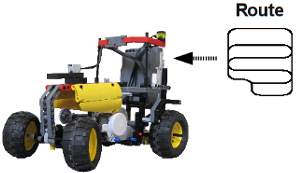
\includegraphics[height=3.6cm]{TractorSimple/tractorSimple_Overview.png}
  \label{subfig:tractorSimple_a}
  }
  \hspace{1cm}
  \subfigure[Sketch of the micro-tractors steering and drive components.]{
  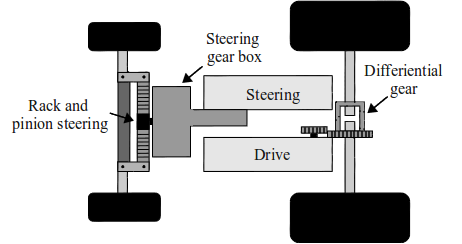
\includegraphics[height=3.6cm]{TractorSimple/tractor_sketch.png}
  \label{subfig:tractorSimple_b}
  }
\end{figure}

Two DC-motors on the micro-tractor are used to steer the front-wheels
and drive the back-wheels (see figure \ref{subfig:tractorSimple_b}).
%A localized reference system based on the motor-encoders and IMU (Iertial Measurement Unit) values is used to determine the current position.
The current route segment (straight line, turn/circle) in the
pre-planned route is followed until the controller determines a new
segment must be loaded.  When the micro-tractor has fished the
pre-planned route, it stops and ends the execution phase.

\section{External Links}
The purpose of this model was to model the general behaviour of the
micro-tractor, when running a pre-planned route and compared
successfully against the real system in \cite{Christiansen&12a}.
Using the \DESTECS model for tuning optimized control parameters for
the route-following algorithm was determined.

\section{Contract}
The primary purpose of this model is to simulate the behavior of the
micro-tractor, when following a route-plan.  Different P-control
parameter values can be set to determine the influence on the system
output.  P-control factor is set using shared variable of type
\keyw{real} found in the contract as: \texttt{P\_k}.  The voltage
output to the motors can change to simulate different input voltage
level to the motors.  Recommended voltage level is between
\textbf{7.4-9.0} V, which is normal battery operation range.  To set
the output voltage in the contract, the parameter
\texttt{Voltage\_Power} of type \keyw{real} should be used.

The contract contains three monitored variables of type \keyw{real}
used to read the rotational-angle of the motor-encoders and the IMU
angle of the tractor: \texttt{ImuOrientation},
\texttt{wheelRotations}, \texttt{steerRotations}.  To control the
motors for the drive and steering system the DE controller uses the
following two control signals of type \keyw{real} in the contract:
\texttt{drivingControl}, \texttt{steering\-Control}.  Finally the
contract contains the route number, used in the system-case for route
following.

\section{Discrete-event}
The DE model consist of the \texttt{Controller} which is the main
thread of control, as well as the task scheduler of the
route-follower.  The route follower \texttt{Route} is used to determine the current
position and delegate the individual route segments to a low-level
controller.  Inputs from the motor-encoders and IMU are used to
determine the current position of the tractor using kinematic
estimates.  Motor output-value rage is equal to the real range found
on the actual micro-tractor.  The low-level controller is a
P-controller used to keep the micro-tractor on the wanted route and
follow a specific lines.

\section{Continuous-time}
The CT model includes a controller block (\texttt{Controller}) which
handles the interface with the DE model.  There are blocks to
represent the motors, the gearing and the wheels for the back of the
tractor, and a separate set of blocks to represent motors, gearing and
wheels for the front of the tractor.  There are separate encoders for
the front and back of the tractor.

The controller produces voltage signals to control both steering and
drive motors on the micro-tractor.  The motor encoders measure the
current speed of the tractor, and the IMU measures the orientation and
feeds this information back to the controller.  The input to the motor
encoders is the motor speed (produced by either the
\texttt{Backend\_motor} or the \texttt{Frontend\_motor}) with some
added noise to model a more accurate system and the output is a count
indicating the number of rotated degrees.  IMU input data is based on
the estimated kinematic position of the micro-tractor modeled in
20-sim and the output is the current angle of the tractor.

20-sim is used to 2D-plot the actual X,Y path the micro-tractor
follows compared to the pre-planned route.  This can be used to
visually evaluate the effect of the current parameter setup.  If the
control parameters are set at random, scenarios will be encountered
where the micro-tractor steers off the pre-planned route.
%A 3D animation is used to visualize the general movement of the micro-tractor with front- and back wheels.

\section{Usage}
To load another route plan change the path to the \keyw{*.csv} file
used to store the plan.  Three example route-plans:
(\texttt{route1.csv},\texttt{route2.csv},\texttt{route3.csv}) are
provided by default to provide the user with an overview of the
capabilities.  Simulation time should be set high for the tool to be
able to run the entire route-plan.  \texttt{route1.csv} requires a
simulation length of between 100-120 sec, depended on the voltage
input.  The format of the route-plane file is the following:

\begin{table}[!ht]
\centering
\begin{tabular}{|c|c|c|}\hline
\keyw{Type} & \keyw{Orientation} & \keyw{distance}\\ \hline
1(Line) & 90 (degrees) & 2 (meter) \\ \hline
2 (Cycle) & -180 (degrees) & X (empty) \\ \hline
\end{tabular}
\caption{Format of the route-plan csv files.}
\label{tab:route_plan_format}
\end{table}

Any route length can be chosen, but be aware that longer routes
require longer simulation time.  To get the tractor to steer an
unpredictable route, provide it with a line route-segment, with an
orientation opposite its own current orientation.

\chapter{ChessWay Simple} \label{chap:chesswaysimple}
\section{Case Description} The ChessWay is a two-wheeled,
self-balancing scooter which utilises a gyroscope to maintain a stable
upright position. The scooter consists of a platform on which the
rider stands, two parallel wheels and a handlebar.  A model of the
scooter can be seen in Fig~\ref{fig:chessWaySimple}.

\begin{figure}[!ht] \centering
\includegraphics{chessWaySimple/chesswaySimple.JPG}
\caption{Image of the ChessWay personal scooter
\label{fig:chessWaySimple}} \end{figure}

The ChessWaySimple model is a simplified and abstracted model of the
scooter.  It features a sensor which can be used to calculate current
forward velocity and an acceleration sensor which can be used to
determine the current angle. Each wheel has its own motor, although
there is a single controller for both motors, so the scooter travels
in a straight line only (see the ChessWay \DESTECS model in Chapter
\ref{chap:chesswaydestecs} for a slightly more complex model that
permits separate inputs to motors). Users simply lean forwards to
increase forward motion.  This is a trivial and simple version of the
ChessWay model; for more advanced versions of the same vehicle we
recommend studying Chapters \ref{chap:chesswaysl} and
\ref{chap:chesswaydestecs}.

%\section{External Links}

%\begin{itemize} %\item Papers/technical reports where the model
%is used %\end{itemize}

\section{Contract} The contract contains four shared state
variables of type {\textbf\ttfamily{real}}. Two monitored variables
are responsible for reading in signals from the sensors used for
calculating velocity (\texttt{v\_in}) and acceleration
(\texttt{a\_in}). Two controlled variables are responsible for
producing a signal to the motors to alter forward velocity
(\texttt{v\_out}) or to make adjustments to the current angle
(\texttt{a\_out}). Both of the controlled variables produce a signal
to power the motors.

\section{Discrete-event} The DE model includes a
\texttt{Controller} class which manages the main thread of
control. The Controller instantiates two \texttt{IActuatorReal}
abstract classes, to represent the actuator signal for adjusting
vertical position (\texttt{acc\_out}) and the actuator signal for
adjusting forward velocity (\texttt{vel\_out}). It also instantiates
two \texttt{ISensorReal} abstract classes to represent input signals
from the velocity sensor (\texttt{vel\_in}) and the acceleration
sensor (\texttt{acc\_in}). At run-time, the \texttt{Actuator} class
provides a concrete implementation of \texttt{IActuatorReal} and the
\texttt{Sensor} class provides an implementation of
\texttt{ISensorReal}.

The ChessWay scooter implements a closed feedback loop to produce the
self-balancing functionality. The current angle at any one time is
calculated (based on the input from the \texttt{acc\_in} class that
represents the gyroscope's readings), and then based on this, the
scooter's motor is fed a signal to make corrections and ensure the
scooter stays upright.

The \texttt{System} class deploys the \texttt{Controller} onto a
single CPU.

\section{Continuous-time} On the top level of the hierarchy, the
model consists of three main blocks: the controller (the
\texttt{cosim} part of the model), the plant and a block used for
\texttt{IO} which resides in between the \texttt{cosim} and the
plant. The controller handles the passing of variables to/from the DE
model. The plant block contains three elements, to represent the axis,
the person frame (the unit consisting of the platform and handlebar)
and the wheels. And finally the \texttt{IO} block primarily contains
D-A and A-D conversion functionality.

\section{Usage}
The ChessWay Simple model is designed to be a simple introduction to a
more complex version of the same scooter (see Chapter
\ref{chap:chesswaydestecs}).  Running a simulation of the Simple model
demonstrates how the scooter responds to small changes in velocity by
altering signals to the actuators so that it can maintain an upright
position by way of many small corrections.

\chapter{ChessWay SL} \label{chap:chesswaysl}

\section{Case Description}
The ChessWaySL model is an extension of the previous model (see
Chapter \ref{chap:chesswaysimple}), and acts as a bridge between the
very simple model presented there and the much more complex model of
the same scooter which is presented in the following chapter (Chapter
\ref{chap:chesswaydestecs}).  The model in this chapter includes the
same basic features of a self-balancing scooter described in Chapter
\ref{chap:chesswaysimple}.  However, in this model we are beginning
the process of adding some extra safety features, additional controls
and some fault tolerant functionality. As with the previous model, the
ChessWaySL scooter consists of a platform on which the rider stands,
with two parallel wheels and a handlebar. There is an ignition switch
which the user can use to power the system down explicitly. There is
also a removable safety key device, which is always inserted into a
slot in the handlebar unit while the scooter is in use. At the same
time the safety key will be attached to the user's wrist by a cord, so
that if the user is unfortunate enough to fall off the scooter, the
safety key will be pulled away from its slot in the handlebar
unit. The removal of the safety key can therefore assumed to mean that
the scooter is riderless, and the vehicle must immediately come to a
safe, stationary position.

A distributed controller architecture was chosen for the more advanced
ChessWay, whereby each wheel has its own controller. Each motor
controller is guarded by a so-called safety monitor, which has the
task to intervene and put the system in a fail-safe state in case any
fault is detected. The failsafe state condition for the ChessWay is
the situation where neither motor is actuated. Furthermore, the system
should be able to recuperate from such an intervention and return to
normal operating mode, in case the root cause of the fault has been
removed.  Figure \ref{fig:controllerstates} shows the states and
transitions we require for the controller, and Figure
\ref{fig:plantstates} shows the events and transitions needed for the
plant.
\begin{figure}[!ht ]
\centering
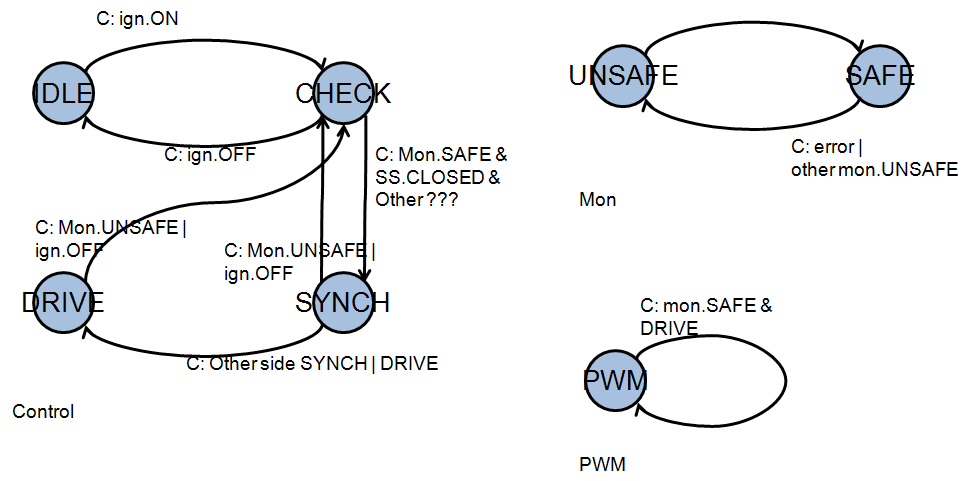
\includegraphics[width=1\textwidth]{chessWaySL/StatesForController.png}
\caption{States and transistions needed for the ChessWay controller model
\label{fig:controllerstates}}
\end{figure}

\begin{figure}[!ht ]
\centering
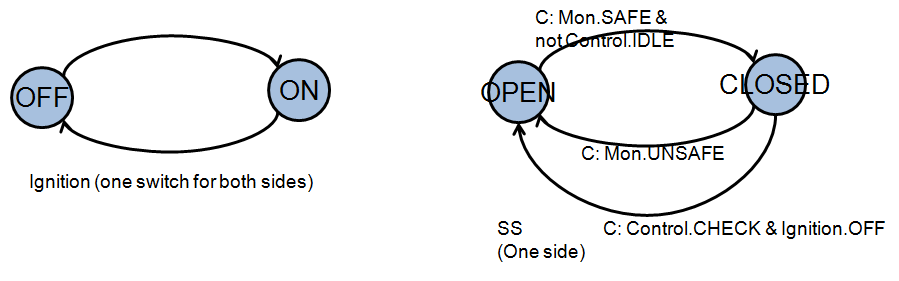
\includegraphics[width=1\textwidth]{chessWaySL/StatesForPlant.png}
\caption{States and transistions needed for the ChessWay plant model
\label{fig:plantstates}}
\end{figure}

In order to develop the simple version of the model (Chapter
\ref{chap:chesswaysimple}) into a model that incorporates all of the
above features, some key design questions must be answered:

\begin{itemize}
\item What constitutes the system?
\item What constitutes the environment?
\item What should constitute the DE side of the simulator?
\item What should constitute software in the controller?
\item What is the minimum number of sensors we need and what is
  necessary for the plant?
\end{itemize}

In order to answer these questions, engineers initially adopt a
DE-first approach, designing the DE side of the model only and
assuming that there is a CT model available which is always correct.
This allows them to concentrate on the discrete event changes that
will be encountered during start-up and shut down, and during
fault-handling and recovery.  The added value of the intermediate
model is that is focuses on state changes only: it shows which sensors
are deeded to be able to detect certain faults; it changes state from
detecting a fault to a safe sate and tries to recover to an
operational state; and it shows the interaction between user and
device.  We present the intermediate, DE-only model in this chapter,
and we present a more complete version of the model with a
fully-implemented CT model in Chapter \ref{chap:chesswaydestecs}.
\section{Defining Data Types}
The first step is to define a set of data types which will act as a
convenient vocabulary in our model.  Simple types (omitted here) for
describing properties from the physical domain start with a capital
\textbf{R} and for the sensed properties we use a prefix
\textbf{S}. The actuator types are preceded by \textbf{A}.  The safety
monitor observes the system health and manages variables of type
\texttt{SafetyMode}.  The controller operates the system and manages
variables of type \texttt{OperatingMode}.

\begin{vdm_al}
	types
		Plant ::
			poleAngle : RPoleAngle
			angleVel : RAngleVel
			safetyKey : RSafetyKey
			powerSwitch : RPowerSwitch
			pwmL : RPwm
			pwmR : RPwm
			safetySwitchL : RSafetySwitch
			safetySwitchR : RSafetySwitch;

		Sensors ::
			ignition : SPowerSwitch
			poleAngle : SPoleAngle
			angleVel : SAngleVel
			safetyKey : SSafetyKey;

		Actuators ::
			pwm : APwm
			safetySwitch : ASafetySwitch;

		Controller ::
			mode : OperatingMode;

		Monitor ::
			mode : SafetyMode;
\end{vdm_al}

The structured types show that the \texttt{Plant} type holds the
actual physical properties, while \texttt{Sensors} contains the
observed values. The real and observed values may differ due to
timing, as the real physical property changes in real-time while the
sensed values only changes when triggered to do so. And furthermore,
the values may differ due to sensor faults. A similar argument holds
for the actuators.

\section{Defining State}
We can now define the state of our model (some states are omitted
here).

\begin{vdm_al}
state Sigma of
	-- real world
	plant  : Plant

	-- modelled world
	sens  : Sensors
	actL  : Actuators
	actR  : Actuators
	ctrlL : Controller
	ctrlR : Controller
	monL  : Monitor
	monR  : Monitor

	-- keep track of the error state
	errors : map ErrorTypes to bool
\end{vdm_al}

Note that the variable \texttt{plant} represents the physical system
properties.  The \texttt{sens} variable is used to hold the sampled
sensor value at some specific point in time, while the variables
\texttt{actL} and \texttt{actR} hold the most recent control signal
which is send to the motors that drive a wheel each.  Finally there is
a pair of \textit{controllers} and a pair of \textit{monitors}.  The
controller resembles the digital controller and the monitor represents
the safety monitor for that controller. The \texttt{plant} and
\texttt{sens} variables occur once, while all other system elements
occur twice, for the left (\textbf{L}) and the right (\textbf{R})
wheel respectively. The controller and monitor variables are
containers for the controller and monitor state machines. They will
become the core processes in co-simulation and in the implementation.

\section{Defining Auxiliary Functions}
We can now define some auxiliary functions and operations that can be
used as encodings of transitions in a state machine.  Using some
simple functions (omitted here) to read sensors, whereby we treat the
user interface button (on/off switch) as an ordinary sensor, we can
now define the transition engine that is at the heart of the
controller state machine.

\begin{vdm_al}
  -- process to migrate from state to state = statemachine
  switchState : Controller * Monitor * Actuators *
    Controller * Monitor ==> OperatingMode
  switchState(c, m, act, cOther, mOther) == (
      -- check monitor first
      -- check ignition
      -- change state
      cases c.mode :
        <IDLE> ->  if sens.ignition = <OFF>
                   then return <IDLE>
                   else return <CHECK>,
        <CHECK> -> if sens.ignition = <OFF>
                   then return <IDLE>
                   else if m.mode = <SAFE> and
                           act.safetySwitch = <CLOSED>
                        then return <SYNC>
                        else return <CHECK>,
        <SYNC> -> ( if m.mode = <SAFE> and
                       mOther.mode = <SAFE> and
                       ( cOther.mode = <SYNC> or
                         cOther.mode = <DRIVE> )
                    then return <DRIVE>;
                    if m.mode <> <SAFE> or
                       mOther.mode <> <SAFE>
                    then return <CHECK>;
                    return <SYNC> ),
        <DRIVE> -> if m.mode <> <SAFE> or
                      sens.ignition = <OFF>
                   then return <CHECK>
                   else return <DRIVE>
      end;
      -- default return value
      return <CHECK>;
    );
\end{vdm_al}

The core process of the controller. The On/Off switch makes the state
switch between \textsf{IDLE} and the other states.  The \textsf{CHECK}
state is the landing place after switching on and after detection of
an error. The \textsf{SYNC} state is introduced to synchronize between
the left and right controller. The controller being in a safe state, a
check is made before powering the motor that the other side is in the
same state as well. If so then both will move to the \textsf{DRIVE}
state and power the two motors. In case of an error, or desire to
switch off, the mode will change to \textsf{CHECK} again.

\section{Usage}
Finally,
we can create an operation that simulates the behavior of the state
machine.
\begin{vdm_al}
  -- simulator
  simulator : () ==> ()
  simulator() == (
    dcl tick : int := 0;

    while tick < 25 do (
      IO`print(tick);

      -- script
      if tick = 2
        then switchOn();
      if tick = 4
        then pullSafetyKey();
      if tick = 7
        then restoreSafetyKey();
      if tick = 16
        then pullSafetyKey();
      if tick = 19
        then restoreSafetyKey();
      if tick = 23
        then switchOff();

      -- read sensor values
      sens := sense();

      -- sense & monitor & activate
      if ctrlL.mode <> <IDLE>
        then (
          monL.mode := switchMonitorState(ctrlL);
          actL.safetySwitch :=
            switchSafetySwitch(monL.mode, ctrlL.mode);
          actL.pwm := pwmOut(ctrlL.mode, monL.mode, sens);
          plant.pwmL := setPwm(actL);
          plant.safetySwitchL := setSafetySwitch(actL);
      );
      if ctrlR.mode <> <IDLE>
	    then (
          monR.mode := switchMonitorState(ctrlR);
          actR.safetySwitch :=
            switchSafetySwitch(monR.mode, ctrlR.mode);
          actR.pwm := pwmOut(ctrlR.mode, monR.mode, sens);
          plant.pwmR := setPwm(actR);
          plant.safetySwitchR := setSafetySwitch(actR)
        );

      -- control
      ctrlL.mode := switchState(ctrlL, monL, actL, ctrlR, monR);
      ctrlR.mode := switchState(ctrlR, monR, actR, ctrlL, monL);

      tick := tick + 1;
    );
  )
end Chessway
\end{vdm_al}

The simulator process demonstrates that changes in the environment
(user input) make the system pass the states in a desired
manner. Switch \textsf{On} and \textsf{Off}, and pulling the safety
key at specific moments to trigger errors at all times in the state
machine.  Code coverage analysis showed that initial tests missed some
of the possible execution paths. By adding more tests manually, more
confidence is gained in the design and analysis. The experiments show
that this model is at the right level of being able to add faults and
to analyse fault handling.


\chapter{ChessWay DESTECS} \label{chap:chesswaydestecs}
\section{Case Description} The ChessWayDESTECS model is an
extension of the previous two models (see Chapters
\ref{chap:chesswaysimple} and \ref{chap:chesswaysl}). Like the model
presented in Chapter \ref{chap:chesswaysl}, the vehicle described by
the ChessWayDESTECS model is a self-balancing scooter with two parallel
wheels and a handlebar, an ignition switch and a removable safety key.

The scooter employs sensors to indicate whether the safety key has
been removed from the handlebar unit, or whether the user has switched
off the ignition. There are some differences in how the scooter should
respond when ignition is switched off, or when the safety key is
removed. If the user turns off the scooter, then the model should
first check the current state of the vehicle, and if it is currently
in active motion it should bring it to a safe, stationary position
before deactivating. In contrast, if the safety key is removed from
the handlebar unit, then we assume that the user has fallen from the
scooter and so it should be immediately brought to rest with no need
to check current status.

Unlike the ChessWaySimple model, there are separate controllers for
each of the wheels.  The controllers for the motors are connected
wirelessly, so the model must cope with occasional lost data packets.
As before, there is a sensor which can be used to calculate current
forward velocity of the scooter, and a gyroscope (acceleration) which
can be used to determine the current vertical angle.

\section{Contract} The contract contains six shared state variables of
type {\textbf\ttfamily{real}}. Two monitored variables are responsible for
reading in detected error in velocity
(\texttt{rmsVelocityError}) and the current angle of the
handlebar mast (\texttt{poleAngle}). Four more controlled
variables are responsible for producing signals to the motors to
alter velocity for the left (\texttt{pwmSettingL}) and right
(\texttt{pwmSettingR}) wheels, and for powering the safety key
override on the left (\texttt{safetySwitchL}) and on the right
(\texttt{safetySwitchR}).

The contract also contains 6 display variables, all of type
{\textbf\ttfamily{controlled real}}. The display variables are shared
between the DE and CT models and are available for 3D modelling,
if needed.

Finally, there are two shared design parameters, \texttt{pidGain} and
\texttt{sdpSlip}, the values of which can be set or altered to
simulate different errors.

\section{Discrete-event}  We recommend also reading Chapter \ref{chap:chesswaysl}, which describes the process of implementing this model in more detail.   The DE model includes a number of
classes to designed to represent various sensors, including one each
for \texttt{Gyro}, \texttt{Ignition}, \texttt{SafetyKey},
\texttt{VelocitySensor} and one to detect \texttt{VelocityError} (it's
assumed that the hardware is capable of reporting self-detected
errors). There are also two classes representing actuators:
\texttt{Pid} handles the standard actuators powering the wheels. And
\texttt{SafetySwitch} handles an override of the \texttt{Pid} class,
if the safety key has been withdrawn.

The DE model starts with a \texttt{System} class, which creates
single instances of each of the sensors for monitoring: the
gyroscope; the safety key; the ignition switch; the velocity;
and detected velocity errors. \texttt{System} then creates two
instances of a \texttt{Monitor} class (one for each wheel/motor)
to monitor these sensors and determine the correct current state
for the scooter. \texttt{System} also creates two instances of
the \texttt{RTControl} class, which act as controllers (one for
each motor/wheel). The \texttt{RTControl} instances each have
their own copy of a \texttt{Pid} class (representing the
actuator for activating the motor) and a \texttt{SafetySwitch}
class (for overriding the actuator).

Finally, \texttt{System} also creates a single instance of a
class that represents the wireless data connection. An abstract
class \texttt{Ether} is provided for this purpose along with
several concrete implementations, each of which behaves slightly
differently. Currently the model uses the concrete
implementation \texttt{LossyEther}, which `drops' randomly
selected data packets at runtime.

\section{Continuous-time} The CT model is presented in more
detail than other examples, and several possible 20-sim models
are provided. There are some small variations in detail in each
of the 20-sim models, but for each one the blocks are gathered
into collections of actuators (which receive signals for the
motors driving the wheels and for the safety switch circuit) and
sensors (which produce outputs relating to the current angle,
the velocity and detected error). To maintain a high level of
dependability, we assume that the safety key functionality is
deployed onto a separate CPU to the main plant. Both the main
plant and the safety monitor receive copies of the sensor input;
should the safety monitor detect anything amiss it overrides the
main plant's outputs with its own signal to deactivate the
scooter.

A single block (\texttt{sbsInterface}) handles imports from, and
exports to, the DE model; this block produces outputs for the actuators and
receives inputs from the sensors. In each model a collection of
\texttt{Cycloid} blocks is used to calculate whether the
gyroscope is accurately detecting vertical. A single block
(either \texttt{Chessway} or \texttt{SBS}) represents a detailed
submodel of the plant, and interacts with the actuators, sensors
and error-detecting functionality.

The actuators for each wheel communicate via a wireless
connection in this model, allowing some fault tolerance
behaviour to be tested as the model must cope with packets
occasionally lost in transmission. In the CT model each of the
receivers for the motors is linked to a fault-generating block
that loses occasional packets.

\section{Usage}
This is a complex model, and many scenarios are also possible.  The
DESTECS co-model provides alternative implementations of the
\texttt{Ether} class, for example, which exhibit different behaviours
and may be tried separately to test fault tolerance.  The difference
between activating the safety key and deactivating the ignition can be
seen by changing the script above to shutdown the ignition instead of
removing the safety key.

\subsection{Scenarios}
A simple scenario is provided for the
ChessWayDESTECS model, demonstrating some aspects of the
scooter's safety.

\begin{dcl}[caption=DCL script which activates the scooter and then simulates the removal of the safety key and its replacement]
when time = 0.0 do (de real safetyKeyEnabled := 1.0; );

when time = 0.2 do (de real safetyKeyEnabled := 0.0;);

when time = 0.3 do (de real safetyKeyEnabled := 1.0;);

when de real poleAngle < 0.0-0.2
	or de real poleAngle > 0.2
	do ( print "QUIT ... "; quit; );

\end{dcl}

In this scenario, the safety key is withdrawn from the handlebar
unit (\texttt{when time = 0.2}) and then quickly replaced
(\texttt{when time = 0.3}). The scooter responds to the removal
of the safety key by beginning to shut down, but the replacement
of the key results in abandoning the shut down and the scooter
attempting to recover its stable vertical position. The timings
provided in this scenario should demonstrate that the scooter is
capable of recovering and returning to vertical safely. The
scenario can be altered and executed with different timings,
allowing us to determine the maximum length of time that may
elapse between withdrawing the safety key and replacing it and
still have the scooter recover its upright position.

Another possibility is to try out the gyroscope fault detection
functionality.  The script below simulates the detection of an error
in the gyroscope.

\begin{dcl}[caption=DCL script which activates the scooter and then simulates detection of a fault in the gyroscope]
when time = 0.0 do (de real safetyKeyEnabled := 1.0; );

when time = 0.1 do (de int gyroError := 1;);

when time = 0.13 do (de int gyroError := 0;);
\end{dcl}


% Appendix starts here
\appendix
%\include{ACAAppendixA}


% Bibliography starts here
\backmatter

% Generate bibliography
%\fancyhead[LO]{Bibliography}
\bibliographystyle{alpha}
\label{ch:bib} %label to refer to
\bibliography{../usermanual/dan,comp}
%\cleardoublepage

\end{document}

